\chapter{Tuning MC Simulated Events by Determining Weights}
\label{chap:weights}
\chapquote{Light weight, baby!}{Ronnie Coleman.}
Monte Carlo (\gls{mc}) simulated events are a product from chaining various different software frameworks that use \gls{mc} methods to simulate the interaction and passage of particles through matter.
In particular the simulation of the passage of particles through matter highly relies on a high fidelity of the description of the detector assembly.
At the same time, a meticulous detector description slows down the simulation significantly and neither geometric, nor material specific properties of all sub-components can be known exactly.
For example, it is only possible to measure the magnetic field when the detector is partially disassembled.
The spatial distribution of the magnetic field of the assembled detector, which is a crucial input parameter for the particle simulation, thus already relies on error-prone estimations.
Further shortcomings are inaccurate alignments of detector units or imprecise physical input parameters, such as polarizations of initial state particles.

Some of these effects also limit the resolution of recorded data, but typically affect recorded data and \gls{mc} simulated events differently.
In the end, recorded data and \gls{mc} simulated events will never match exactly.
In particular, it is known that the distributions of transverse momentum \pt and pseudorapidity $\eta$ of simulated \Lb baryons can deviate significantly.

The idea of the following section is to weight simulated \Lb decays w.r.t.\ $\pt(\Lb)$ and $\eta(\Lb)$ in such a way that they match the distribution of recorded data.
When using the same set of selection requirements for simulated and recorded data, the extracted weights are selection independent scale factors (weights) that transform feature distributions of simulated \Lb decays to the corresponding distributions of recorded data.
In particular this means that those weights should not depend on kinematic properties, such as lifetime (and thus track type) of the respective daughters and grand-daughters of the \Lb, and thus are applicable also for different decay modes of the \Lb baryon.\footnote{We further use these weights to correct simulated \Xibz decays and incorporate deviations as a systematic uncertainty.}
In order to minimize trigger dependent deviations we only use \gls{lzero} \gls{tis} triggered \decay{\Lb}{\jpsi\Lz} events to extract weights and use them in a subsequent step for weighting \gls{mc} simulated \decay{\Lb/\Xibz}{\Dz\Lz} events.
%Using \gls{tis} instead of \gls{tos} triggered events minimized trigger dependent deviations of recorded and simulated data.

Properties that deviate between recorded and simulated data due to correlations with $\pt(\Lb)$ or $\eta(\Lb)$ will automatically improve with this technique.
We check this by comparing the momentum distribution $p(\Lb)$ of unweighted and weighted \gls{mc} simulated \decay{\Lb}{\jpsi\Lz} events. 

We try two different strategies for extracting weights.
The former minimizes deviations for both $\pt(\Lb)$ and $\eta(\Lb)$, whereas the latter uses $\pt(\Lb)$ only.
In the subsequent analysis we use the latter approach but incorporate deviations when using the weights obtained with the former strategy as a systematic uncertainty.
A description of the selection criteria used to increase the purity of the \decay{\Lb}{\jpsi\Lz} data samples is given in Sec.~\ref{sec:LbToJpsiLz_sel}.
A detailed explanation and discussion of the two different weighting schemes is given in Sec.~\ref{sec:LbToJpsiLz_w1} and Sec.~\ref{sec:LbToJpsiLz_w2}.
We further briefly motivate the use of sideband subtraction rather than relying on \gls{truthmatching} in Sec.~\ref{sec:LbToJpsiLz_tm_vs_ss}.

\section{The Decay \texorpdfstring{\decay{\Lb}{\jpsi\Lz}}{Λb → J/ψ Λ}}
\label{sec:LbToJpsiLz_sel}
The decay \decay{\Lb}{\jpsi\Lz} is a high statistics channel at \lhcb and was used there in the past to measure for example polarization effects \cite{LbToJpsiLz_polarization}.
Due to its large branching fraction this decay was one of the first discovered \Lb decay channels \cite{LbToJpsiLz_discovery} and measurements of the product of production fraction and branching fraction $f(\decay{\bquark}{\Lb}) \times \BR(\decay{\Lb}{\jpsi\Lz})$  at the \dzero and the \cdf collaborations~\cite{LbToJpsiLz_D0,LbToJpsiLz_CDF} are still used today for determining branching fractions from measurements of \Lb branching ratios.

%The quark transition in \decay{\Lb}{\jpsi\Lz} is \decay{\bquark}{\cquark\cquarkbar\squark} and is thus proportional to the product of \gls{ckm} matrix elements \Vcb \Vcss or $A\lambda^2$ in the \gls{wolfenstein}.
%In the Tab.~\ref{tab:LbToJpsiLz_qtransitions} below, we compare this amplitude in terms of \gls{ckm} matrix elements with the related modes \decay{\Bdsb}{\jpsi\KS}, as well as the respective decays for \decay{\Lb}{\Dz\Lz} and \decay{\Bdsb}{\Dz\KS}. 
%
%\begin{table}[htbp]
%    \centering
%    \caption{Quark transitions and \gls{ckm} matrix elements for \decay{\Lb}{\jpsi\Lz} and related modes.}
%    \label{tab:LbToJpsiLz_qtransitions}
%
%    \begin{tabular}{lll}
%    \toprule
%    Decay & Quark transition & \gls{ckm} matrix elements \\
%    \midrule
%    $\decay{\Lb}{\jpsi\Lz}$ & $\decay{(\bquark\uquark\dquark)}{(\cquark\cquarkbar)(\uquark\dquark\squark)}$ & $\Vcb \Vcss \sim A\lambda^2$ \\
%    $\decay{\Bdb}{\jpsi\KS}$ & $\decay{(\bquark\dquarkbar)}{(\cquark\cquarkbar)(\squark\dquarkbar)}$ & $\Vcb \Vcss \sim A\lambda^2$ \\
%    $\decay{\Bd}{\jpsi\KS}$ & $\decay{(\bquarkbar\dquark)}{(\cquark\cquarkbar)(\squarkbar\dquark)}$ & $\Vcbs \Vcs \sim A\lambda^2$ \\
%    $\decay{\Bsb}{\jpsi\KS}$ & $\decay{(\bquark\squarkbar)}{(\cquark\cquarkbar)(\squark\dquarkbar)}$ & $\Vcb \Vcds \sim A\lambda^3$ \\
%    $\decay{\Bs}{\jpsi\KS}$ & $\decay{(\bquarkbar\squark)}{(\cquark\cquarkbar)(\squarkbar\dquark)}$ & $\Vcbs \Vcd \sim A\lambda^3$ \\
%    \midrule
%    $\decay{\Lb}{\Dz\Lz}$ & $\decay{(\bquark\uquark\dquark)}{(\cquark\uquarkbar)(\uquark\dquark\squark)}$ & $\Vcb \Vuss \sim A\lambda^3$ \\
%    $\decay{\Lb}{\Dzb\Lz}$ & $\decay{(\bquark\uquark\dquark)}{(\cquarkbar\uquark)(\uquark\dquark\squark)}$ & $\Vub \Vcss \sim A\lambda^3$ \\
%    $\decay{\Xibz}{\Dz\Lz}$ & $\decay{(\bquark\uquark\squark)}{(\cquark\uquarkbar)(\uquark\dquark\squark)}$ & $\Vcb \Vuds \sim A\lambda^2$ \\
%    $\decay{\Xibz}{\Dzb\Lz}$ & $\decay{(\bquark\uquark\squark)}{(\cquarkbar\uquark)(\uquark\dquark\squark)}$ & $\Vub \Vcds \sim A\lambda^4$ \\
%    $\decay{\Bdb}{\Dz\KS}$ & $\decay{(\bquark\dquarkbar)}{(\cquark\uquarkbar)(\squark\dquarkbar)}$ & $\Vcb \Vuss \sim A\lambda^3$ \\
%    $\decay{\Bdb}{\Dzb\KS}$ & $\decay{(\bquark\dquarkbar)}{(\cquarkbar\uquark)(\squark\dquarkbar)}$ & $\Vub \Vcss \sim A\lambda^3$ \\
%    $\decay{\Bsb}{\Dz\KS}$ & $\decay{(\bquark\squarkbar)}{(\cquark\uquarkbar)(\squark\dquarkbar)}$ & $\Vcb \Vuds \sim A\lambda^2$ \\
%    $\decay{\Bsb}{\Dzb\KS}$ & $\decay{(\bquark\squarkbar)}{(\cquarkbar\uquark)(\squark\dquarkbar)}$ & $\Vub \Vcds \sim A\lambda^4$ \\
%    \bottomrule
%    \end{tabular}
%\end{table}
%
%Despite the fact that the \gls{ckm} matrix elements listed in Tab.~\ref{tab:LbToJpsiLz_qtransitions} do not take different production rates of the initial \bquark hadrons into account, which contribute non-negligible corrections due to differences in the fragmentation process of \bquark quarks to hadrons, these numbers show two things: \decay{\Lb}{\jpsi\Lz} is much less suppressed than \decay{\Lb}{\Dz\Lz}, whereas background contributions from \Bdb and \Bsb (\glspl{reflection}) are suppressed stronger.
%This makes \decay{\Lb}{\jpsi\Lz} a good candidate for systematic and calibration studies.

In the following we use $\decay{\Lb}{(\decay{\jpsi}{\mun\mup})(\decay{\Lz}{\proton\pim}})$ to extract weights for calibrating the \gls{mc} samples for \decay{\Lb}{\Dz\Lz}.
In order to minimize systematic uncertainties introduced by imprecise simulated trigger responses, only \gls{lzero} \gls{tis} triggered events are used.
In the following we will outline the selection steps which we divide into a preselection, a loose, and a tight selection.
%After applying the outlined selection requirements, we add a brief discussion about their efficiency and end with a short discussion about the distribution of the fit probability.

\subsection{Preselection}
\label{sec:LbToJpsiLz_presel}
We use the full recorded data set of \gls{runtwo} and the \gls{stripping} versions listed in Tab.~\ref{tab:LbToJpsiLz_vstripping}.
Despite their different naming, there are no major differences between different \gls{stripping} versions for the involved \gls{stripping} lines.
\begin{table}[htbp]
    \centering
    \caption{\Gls{stripping} and Reco versions used for reconstructing \decay{\Lb}{\jpsi\Lz}.}
    \label{tab:LbToJpsiLz_vstripping}

    \begin{tabular}{lll}
        \toprule
        Year & \Gls{stripping} & Reco \\
        \midrule
        2015 & \texttt{24r1} & \texttt{15a} \\
        2016 & \texttt{28r1} & \texttt{16} \\
        2017 & \texttt{29r2} & \texttt{17} \\
        2018 & \texttt{34} & \texttt{18} \\
        \bottomrule
    \end{tabular}
\end{table}
Mother particles are reconstructed from daughter particles that passed dedicated \textit{combination} selections.
Properties of the reconstructed mother particle are refined through the vertex fit procedure (no advanced constraints, such as mass or \gls{pv} constraints, are applied) and are subject to dedicated \textit{mother} selections, whereas properties of the respective daughter particles are not updated for subsequent selection steps.
%We use the results of the \gls{stripping} line \texttt{Stripping\-BetaS\-Lambdab2JpsiLambda\-Unbiased\-Line} and refine the \Lb selection with selection steps taken from the \gls{stripping} line \texttt{Stripping\-Lb2D0Lambda0\-\{LL,DD\}\-D02HH\-Beauty2Charm\-Line}.
All selection criteria of the preselection step are listed in Tab.~\ref{tab:LbToJpsiLz_stripsel}.

\subsection{Loose Selection}
\label{sec:LbToJpsiLz_loosesel}
A decay tree fit is applied and the corresponding $\chi^2_\text{DTF}$ distribution\footnote{We will later find that this distribution does not exactly follow the distribution of a \textit{true} $\chi^2$-distribution. For the sake of brevity we will nevertheless refer to it as a $\chi^2_\text{DTF}$.} is used for discriminating combinatorial background.
The $\chi^2_\text{DTF}$ distribution has 8 degrees of freedom (\cf{}~Sec.~\ref{chap:apdx_dtf} for a more detailed discussion):
\begin{itemize}[itemsep=2pt,parsep=2pt]
    \item Mass constraint of \Lz and \jpsi: 2 \gls{dof}
    \item \Lz vertex constraint: 1 \gls{dof}
    \item \decay{\Lb}{\mup\mun\Lz} vertex constraint: 3 \gls{dof}
    \item \Lb \gls{pv} constraint: 2 \gls{dof}
\end{itemize}
The \gls{pv} constraint leverages an ordering of different \gls{pv} hypotheses (if available) w.r.t.\ the goodness of a respective \gls{dtf} (in terms of $\chi^2_\text{DTF}$).
We use this to select only candidates corresponding to the best \gls{pv} hypothesis for the following steps.

The selection criteria of the loose selection are shown in Tab.~\ref{tab:LbToJpsiLz_loosesel} and are grouped into five categories:
Category 1 reduces combinatorial background in the signal region, category 2 ensures disjunct samples w.r.t.\ the track types \gls{LL} and \gls{DD}, and category 3 reduces disk consumption.
The momentum requirements for the final state particles in category 1 are motivated by the fact that particles do have to have a minimal velocity to emit Cherenkov radiation.
Cherenkov light is instrumented in the \gls{rich} detectors for the particle identification at \lhcb.
Particle identification (\gls{pid}) below this threshold and above $\gtrapprox 150\,$\gevc is ineffective.
(These selection requirements supersede the implicit cut-off of $p > 1.4\,$\gevc due to magnet banding.)
The fiducial selection criteria (category 4) are a common choice for initial state particles at \lhcb.
These selections help to avoid known issues with the fidelity of the detector geometry description in the inner- and outermost regions and turned out to be a conservative choice when the overall statistic is sufficient.
Category 5 minimizes the effect of poorly described trigger in simulated data which could potentially introduce a systematic difference between recorded and simulated events.

\begin{table}[htbp]
    \caption{Selection criteria of loose selection used for reconstructing \decay{\Lb}{\jpsi\Lz}. The selections are grouped into five categories which are explained in Sec.~\ref{sec:LbToJpsiLz_loosesel}.}
    \label{tab:LbToJpsiLz_loosesel}

    \centering
    \begin{tabular}{llc}
        \toprule
        Particle & Selection & Category \\
        \midrule
        \proton & $9 \le p \le 150\,$\gevc & 1 \\
        \pion & $3 \le p \le 150\,$\gevc & 1 \\
        \midrule
        \Lz & decay length $\ge 0$ & 1 \\
        \Lz (\gls{LL}) & $z$-pos.\ of decay vertex $<0.5\,$m & 2 \\
        \Lz (\gls{DD}) & $z$-pos.\ of decay vertex $\ge 0.5\,$m & 2 \\
        \midrule
        \Lb & $5.47 \le m \le 5.77\,\gevcc$ & 3 \\
        \Lb & $2 \le \eta \le 4.5$ & 4 \\
        \Lb & $\pt \le 20\,\gevc$ & 4 \\
        \Lb & \gls{lzero} \gls{tis} events only & 5 \\
        \bottomrule
    \end{tabular}
\end{table}

The data samples are split w.r.t.\ the different track types of the \Lz daughters which are referred to as \gls{LL} and \gls{DD}.
%In light of the available statistic mixed states, such as LD tracks, are not taken into account.
%In Fig.~\ref{fig:mLbToJpsiLz_loosesel} we show the invariant mass of \Lb candidates, reconstructed from recorded data.
In order to optimize a \gls{fom}, we define a signal region spanning $5.58 \le m(\jpsi\Lz) \le 5.66\,\gevcc$.
Events outside this region (upper and lower sideband) are considered pure combinatorial background, whereas events inside the signal region are considered to be an admixture of signal and (combinatorial) background events.
Physical background processes are neglected in this part of the analysis since no visible contributions are visible in the invariant mass distributions.% shown in Fig.~\ref{fig:mLbToJpsiLz_loosesel}.

%\begin{figure}[htbp]
%    \centering
%    \begin{subfigure}[b]{.49\textwidth}
%        \centering
%        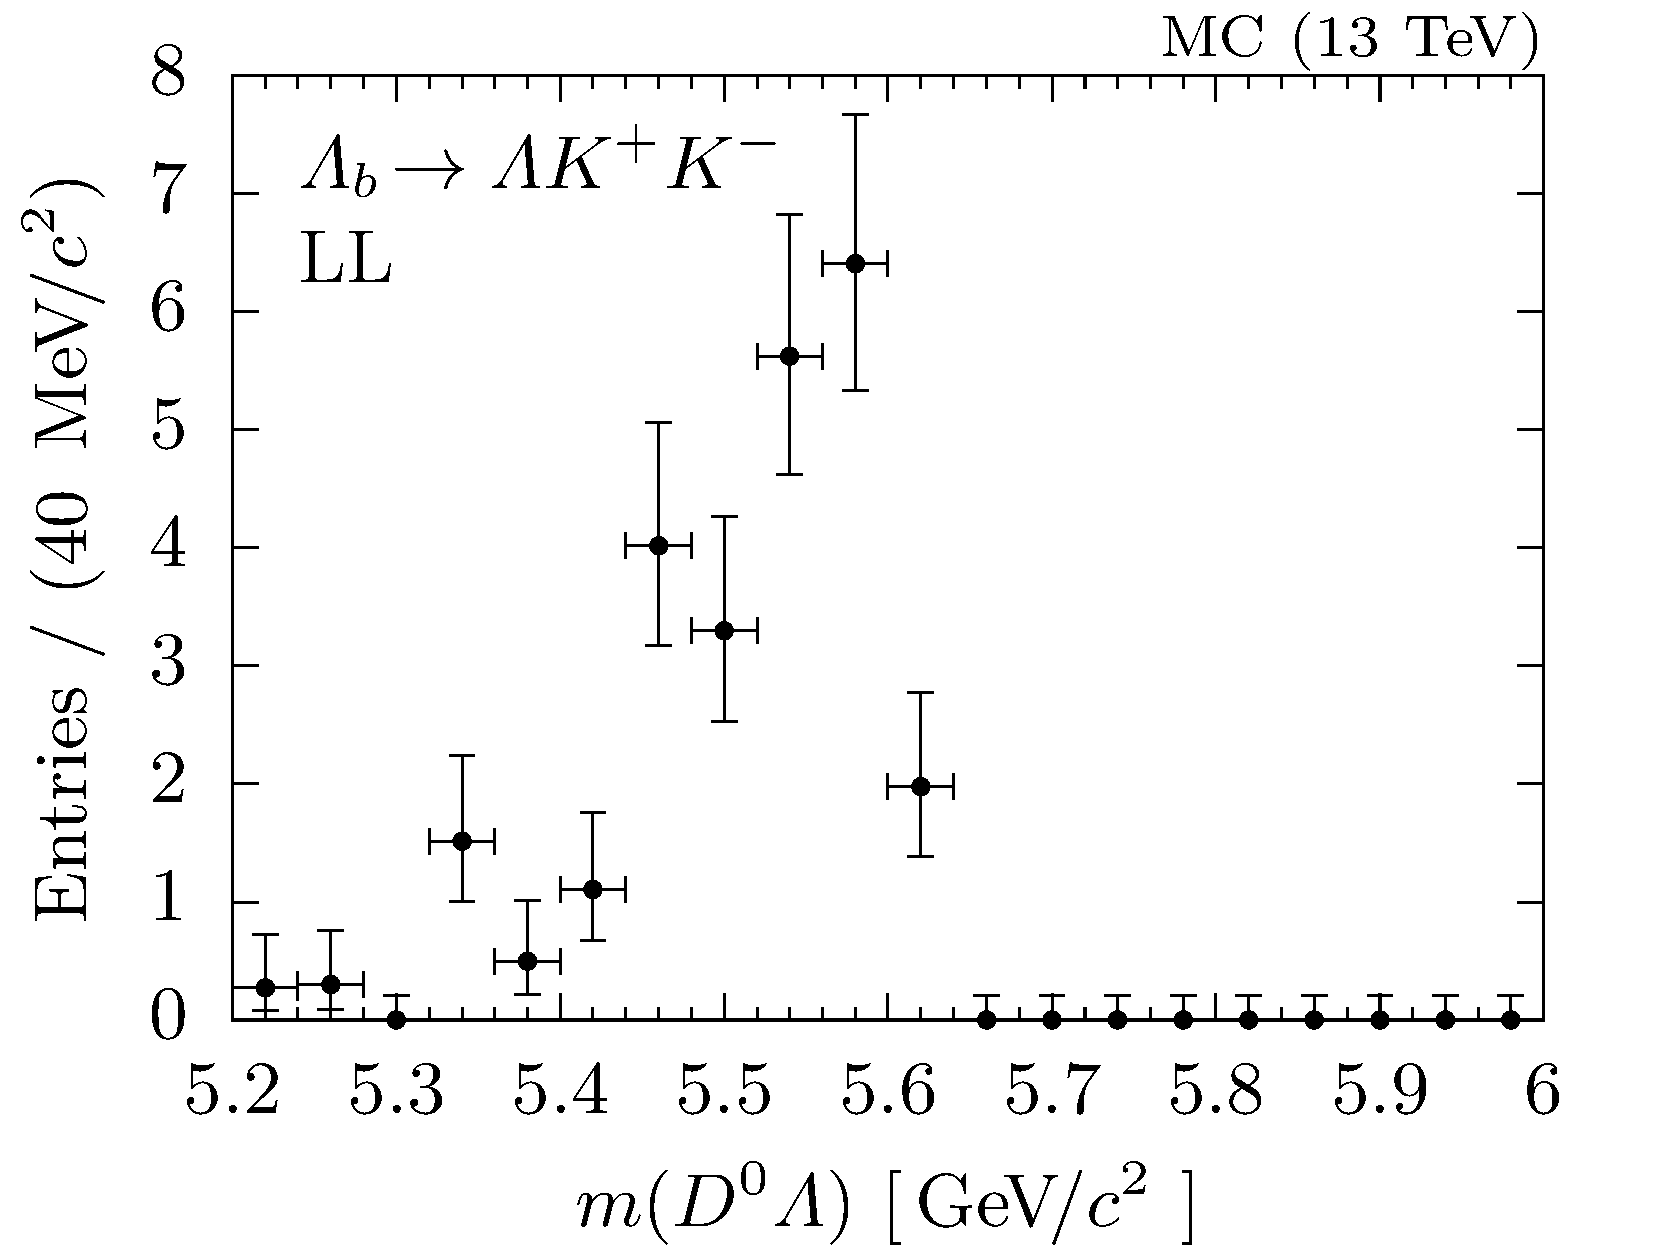
\includegraphics[scale=1.]{Lb2JpsiLz_weighting/hLbM_LL.png}
%        \caption{\Lz candidates rec.\ from \gls{LL} tracks}
%    \end{subfigure}
%    \begin{subfigure}[b]{.49\textwidth}
%        \centering
%        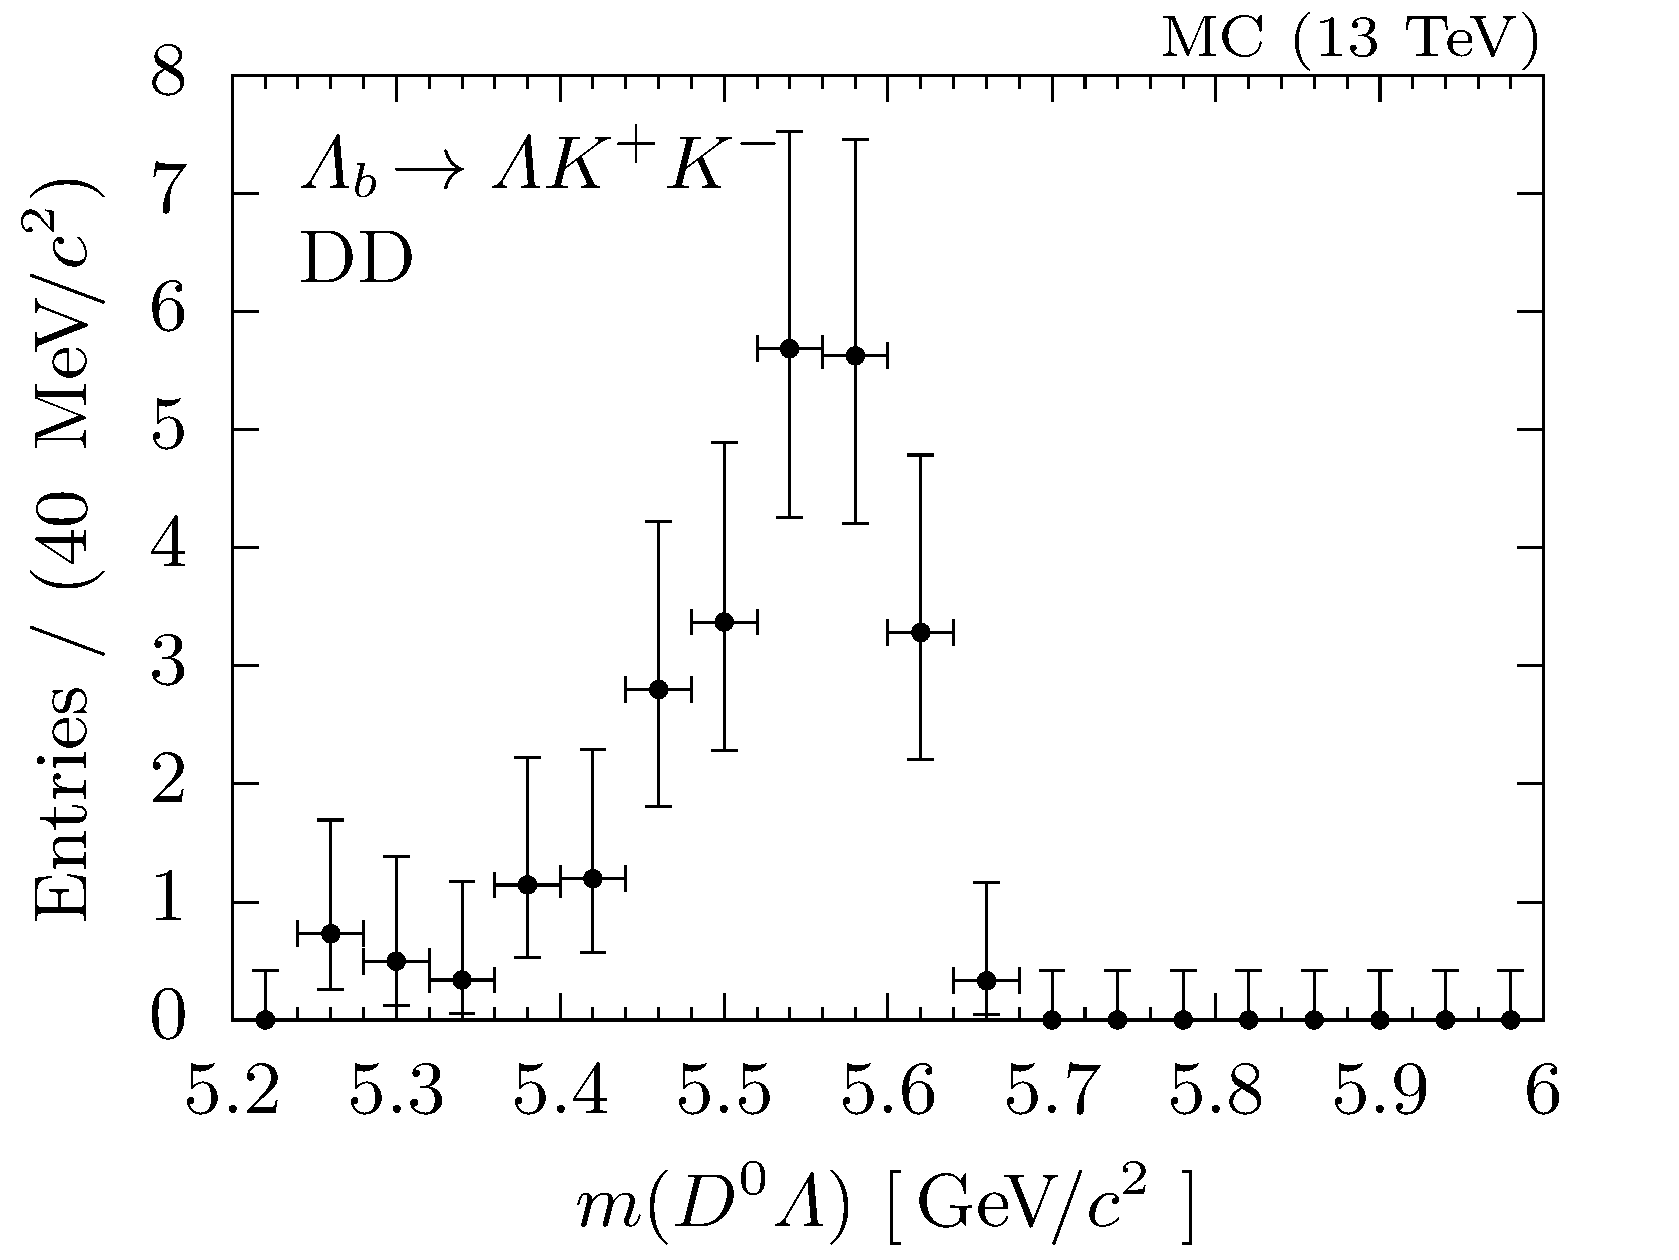
\includegraphics[scale=1.]{Lb2JpsiLz_weighting/hLbM_DD.png}
%        \caption{\Lz candidates rec.\ from \gls{DD} tracks}
%    \end{subfigure}
%    \caption{Combined invariant mass of \jpsi and \Lz candidates after loose selection from recorded data. (Including \gls{lzero} \gls{tis} only requirement.) The dashed lines indicate the \Lb signal region that is used for optimizing a \gls{fom} as part of the tight selection.}
%    \label{fig:mLbToJpsiLz_loosesel}
%\end{figure}

\subsection{Tight Selection}
The objective of the tight selection is to maximize the signal significance as the \gls{fom} for $n_\text{sig}$ signal events and $n_\text{bkg}$ background events in the defined signal region,
\begin{equation}
    \label{eq:fom_LbToJpsiLz}
    \mathrm{FoM} := \mathrm{FoM}(n_\text{sig}, n_\text{bkg}) = \frac{n_\text{sig}}{\sqrt{n_\text{sig} + n_\text{bkg}}} \,.
\end{equation}

The signal significance is maximized for selection requirements w.r.t.\ the $\chi^2_\text{DTF}$ distribution of the \gls{dtf} and the flight distance significance of the \Lz baryon, where the latter is defined as the flight distance $\mathrm{FD}(\Lz)$ over the corresponding standard deviation $u_\mathrm{FD}(\Lz)$ of the \Lz baryon,
\begin{equation*}
    \text{\Lz flight dist. sig.} := \frac{\mathrm{FD}(\Lz)}{u_\mathrm{FD}(\Lz)} \,.
\end{equation*}

The cumulative distributions for both of these features are shown in Fig.~\ref{fig:chi2dtf_LbToJpsiLz} and Fig.~\ref{fig:LzFDs_LbToJpsiLz} for recorded data in the defined signal region and \gls{mc} simulated events.
The cumulative distribution of $\chi^2_\text{DTF}$ indicates a strong separation power between signal and background events, whereas the cumulative distributions of the \Lz flight distance only show minor differences between recorded data and simulated events, hinting towards a low background contamination for the \Lz baryon, \ie{}, the background in $m(\jpsi\Lz)$ predominantly consists of combinatorial background events with genuine \Lz baryons.

\begin{figure}[htbp]
    \centering
    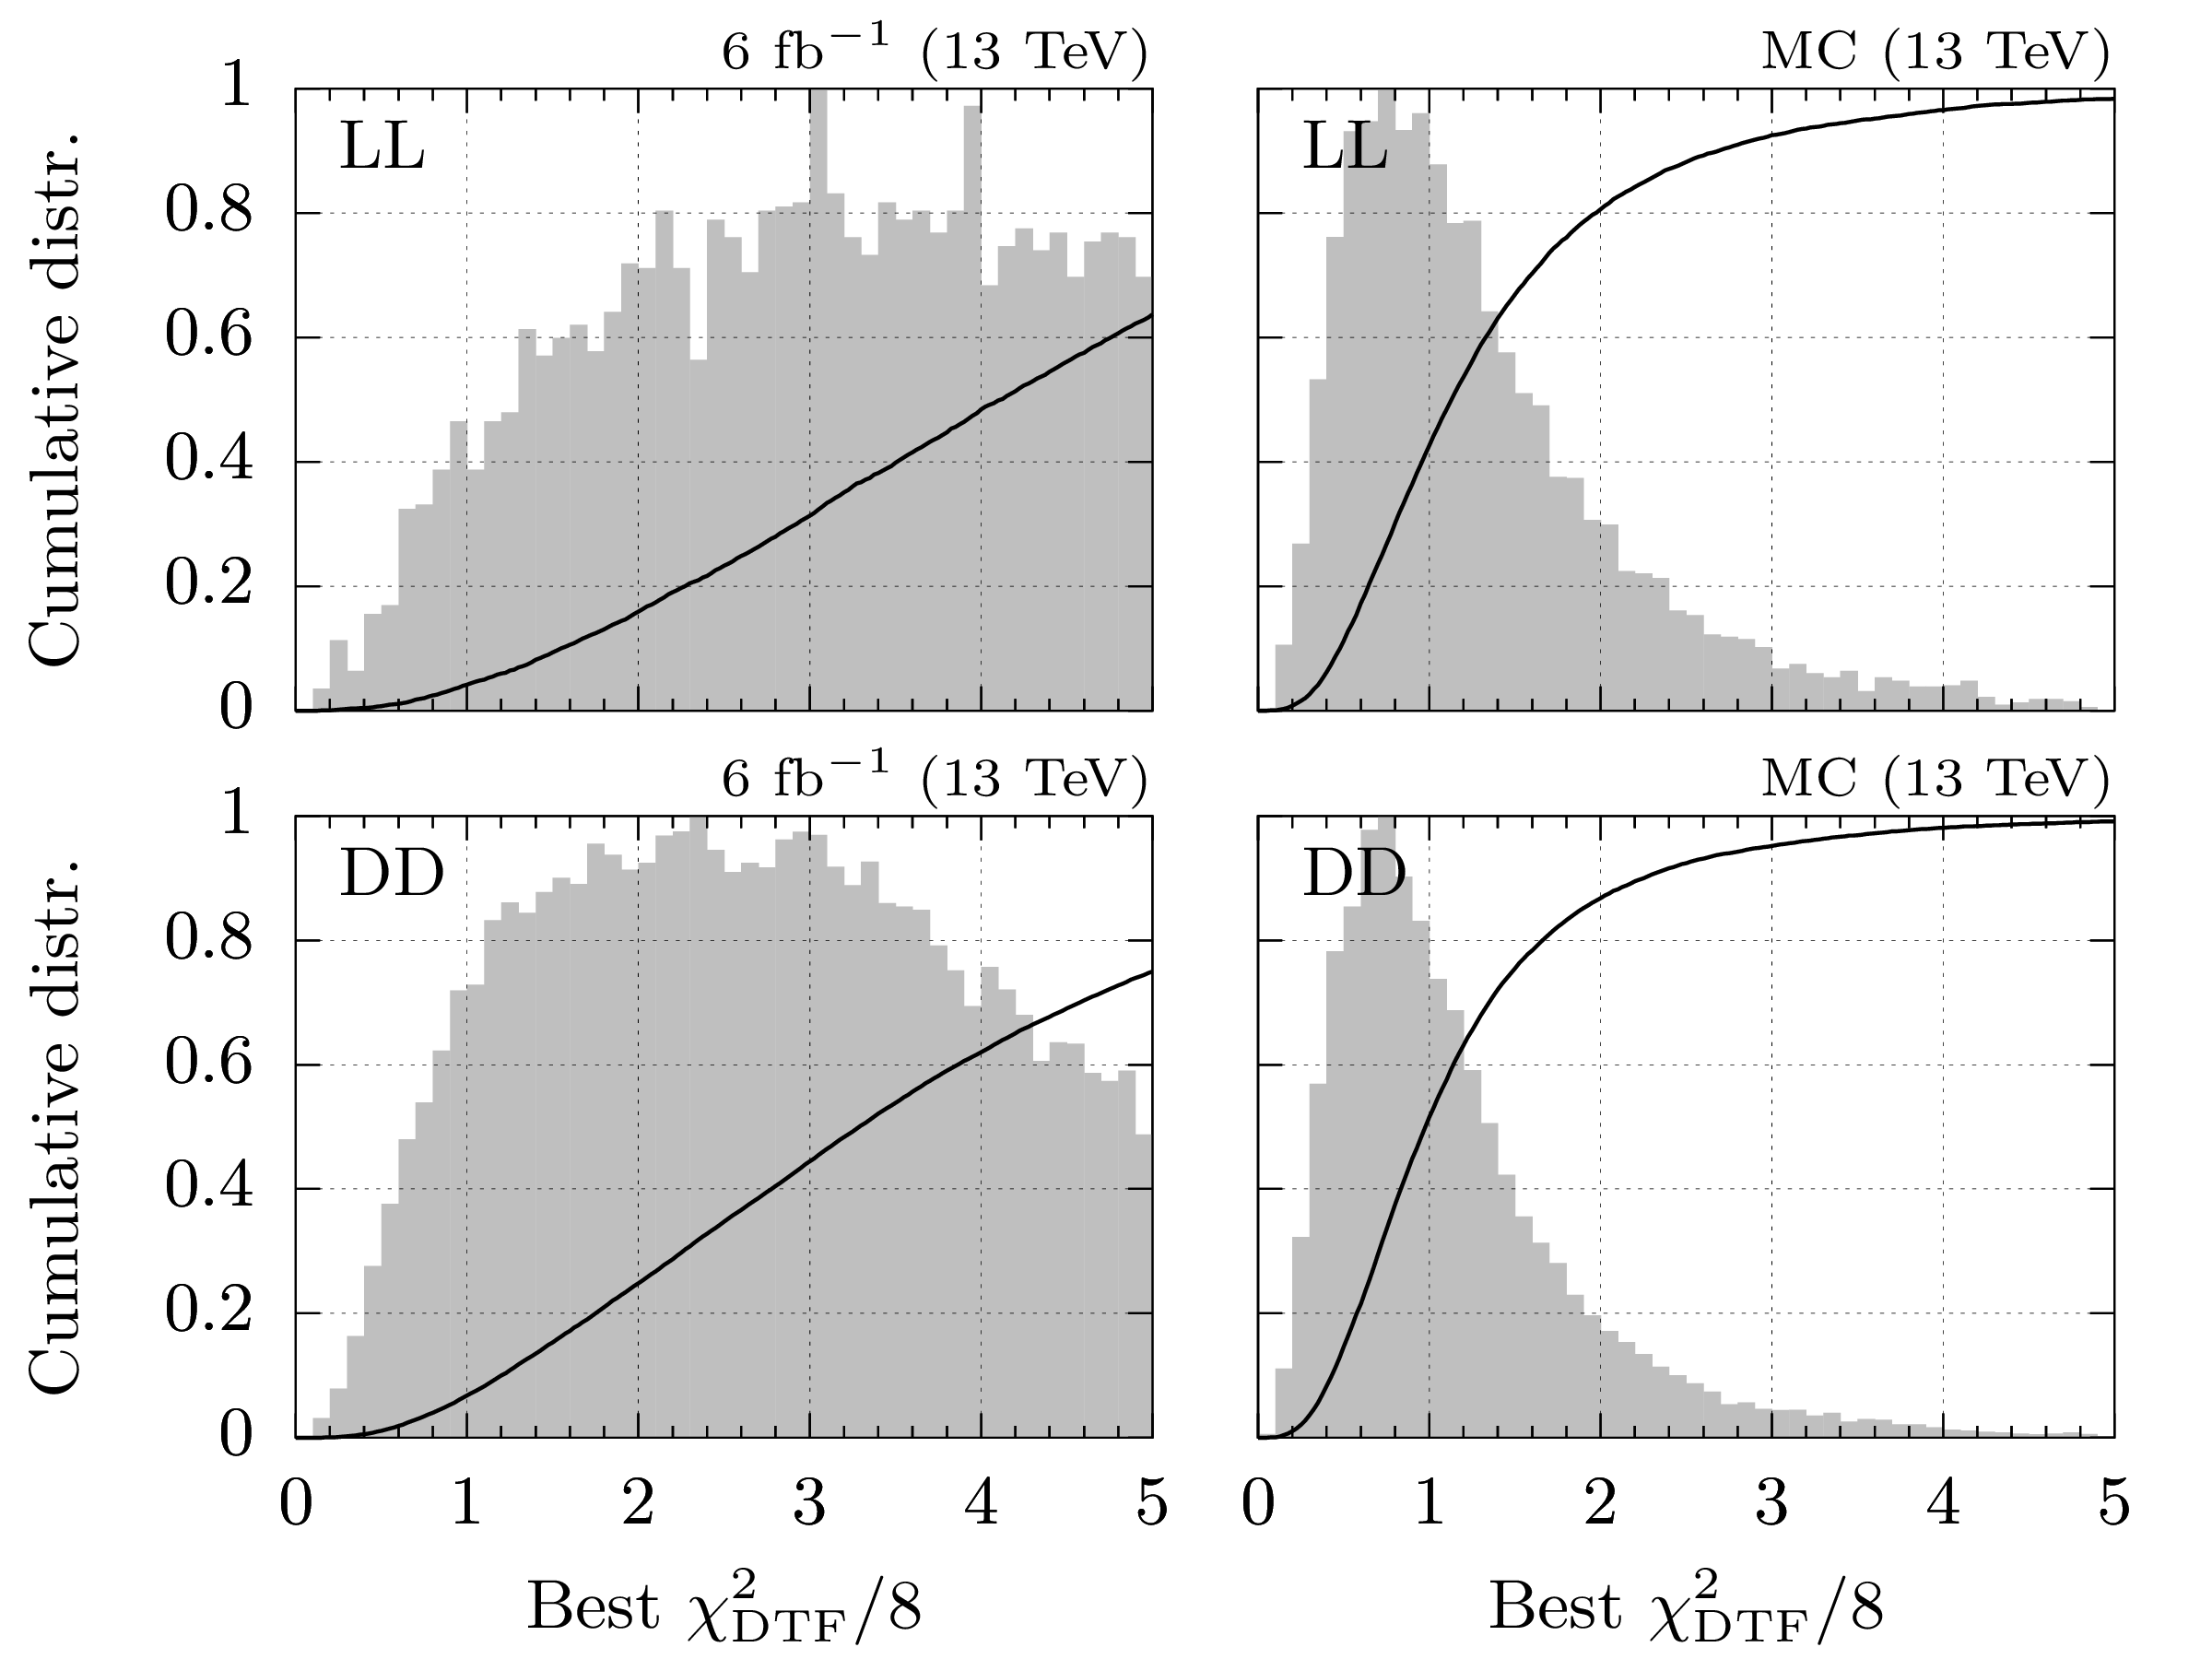
\includegraphics[scale=1.]{Lb2JpsiLz_weighting/chi2.png}
    \caption{Cumulative distribution (solid line) of the $\chi^2_\text{DTF}$ distribution over \gls{dof} for different track types (top and bottom), and for recorded data in the defined signal regions (left) and \gls{truthmatched} simulated events in the signal region (right). The gray shaded areas indicate the corresponding distributions of $\chi^2_\text{DTF}/\mathrm{\gls{dof}}$.}
    \label{fig:chi2dtf_LbToJpsiLz}
\end{figure}

\begin{figure}[htbp]
    \centering
    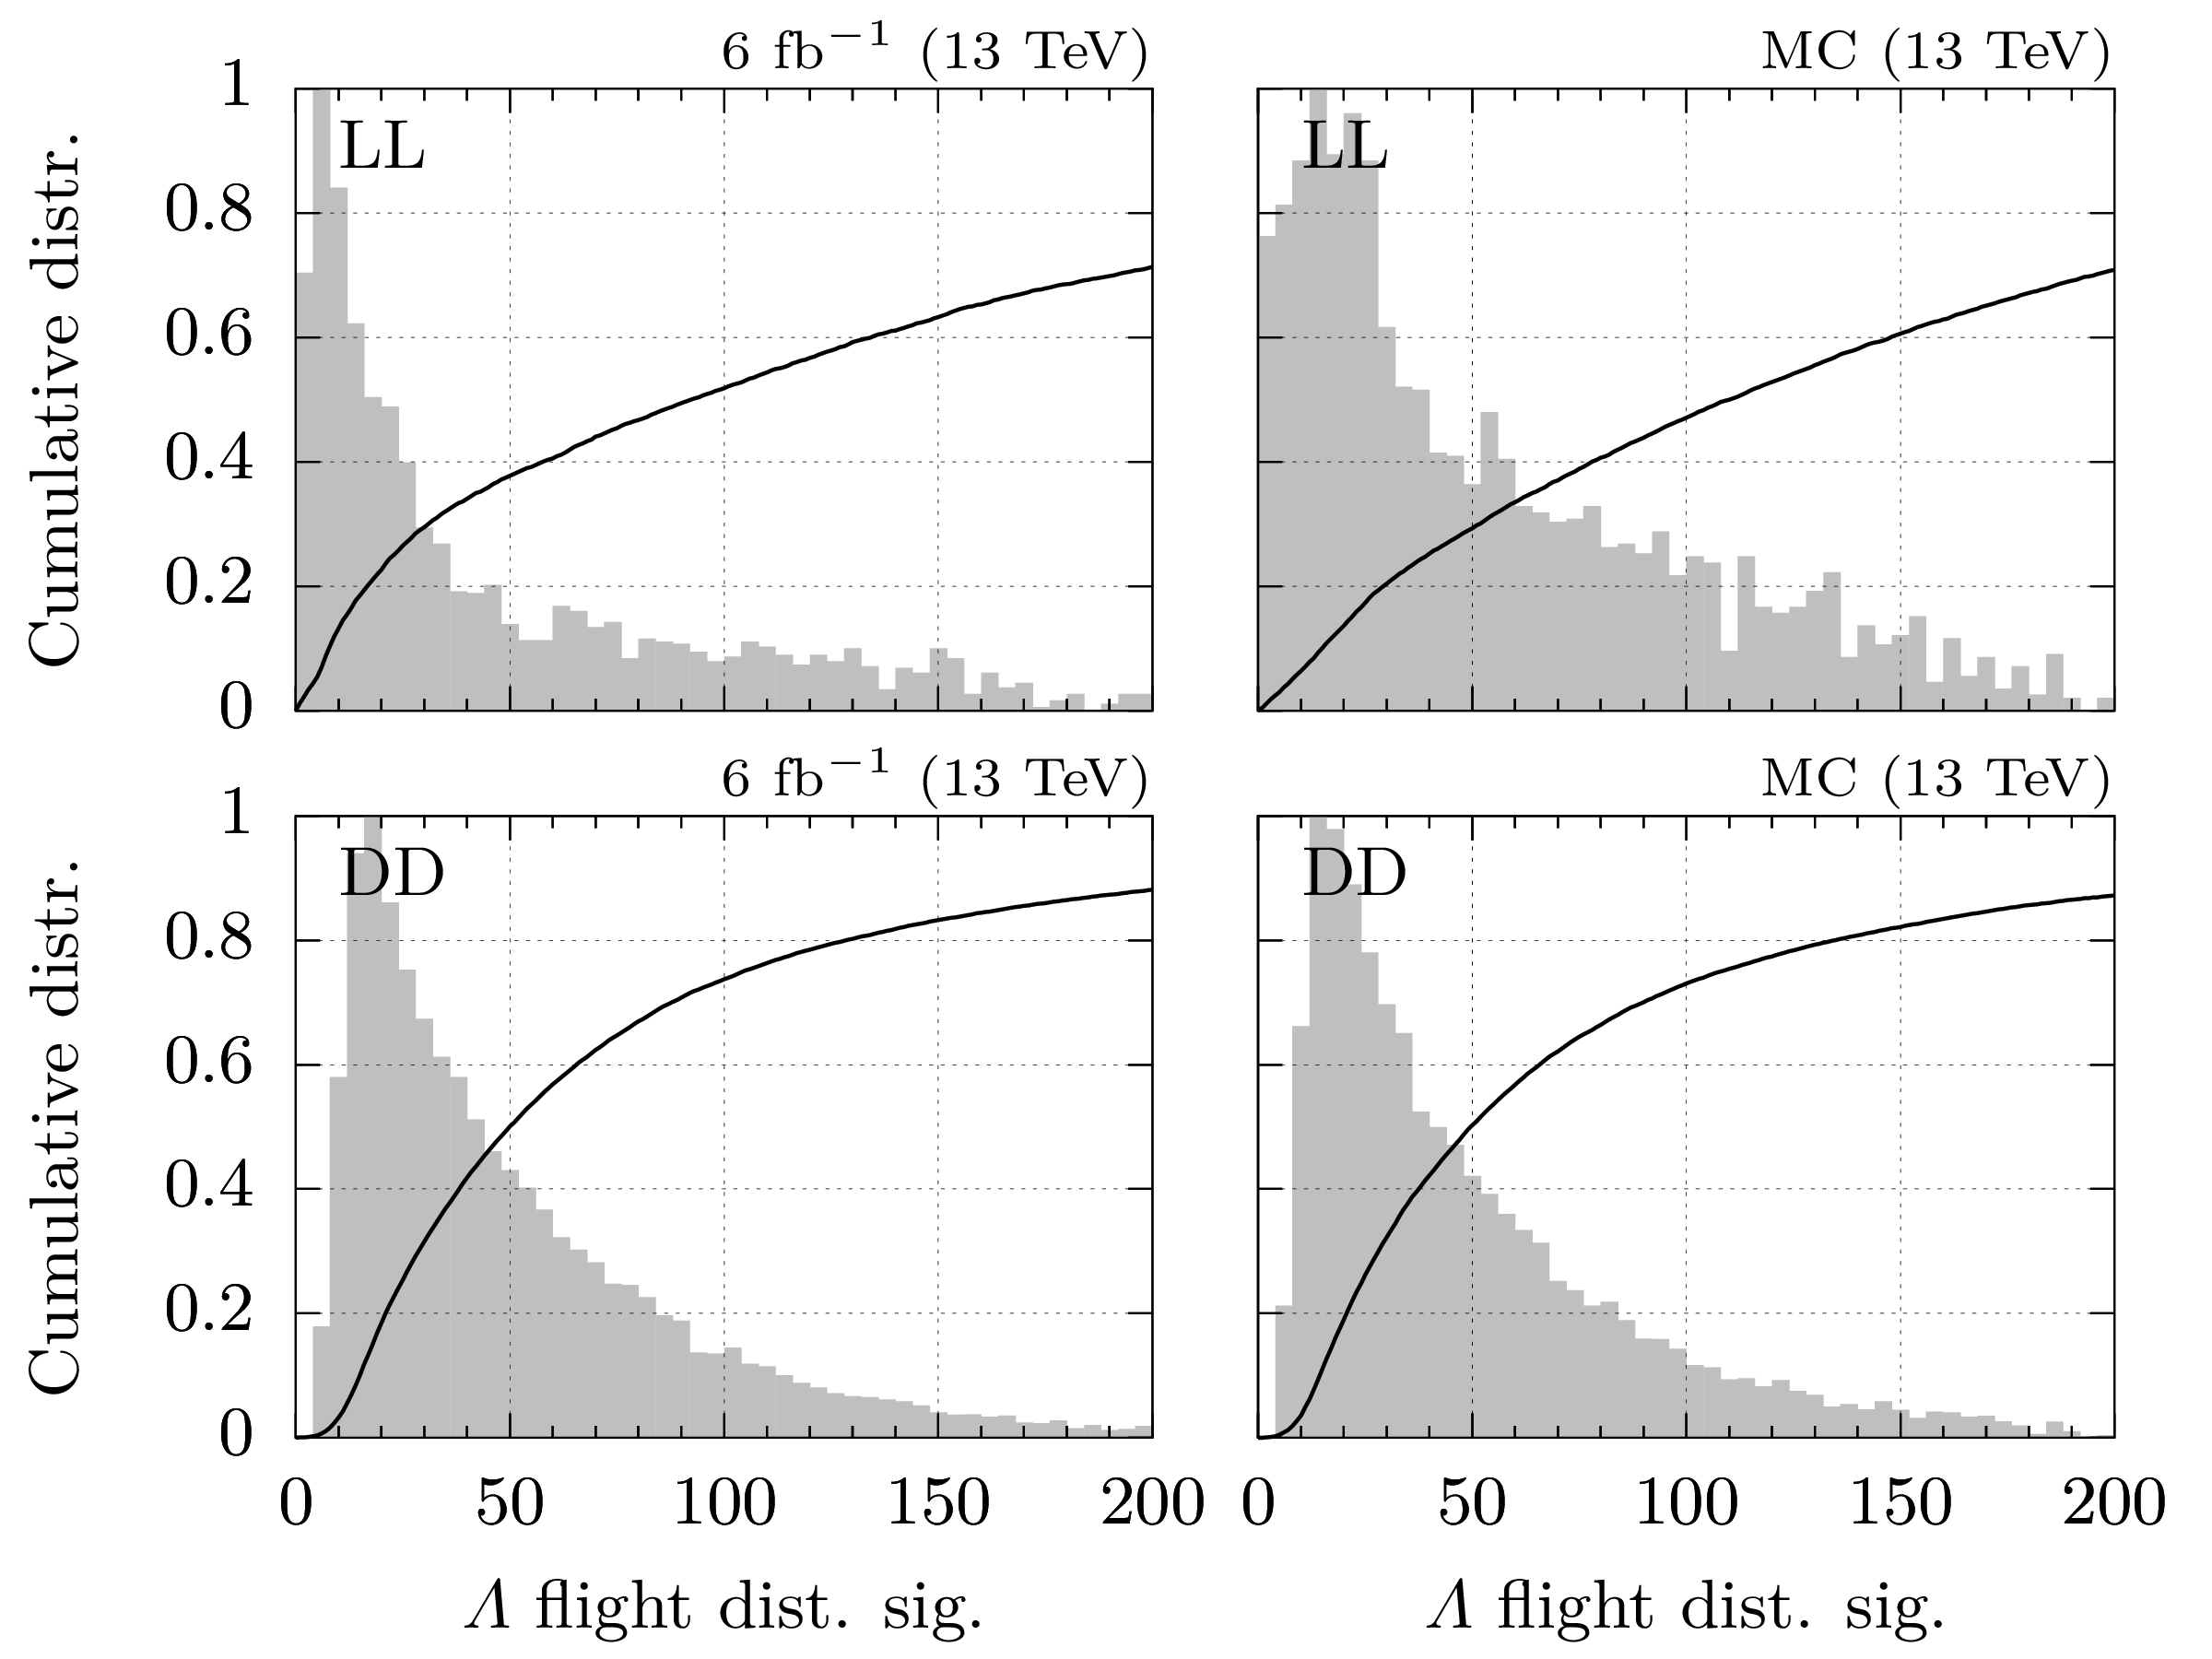
\includegraphics[scale=1.]{Lb2JpsiLz_weighting/LzFDs.png}
    \caption{Cumulative distribution (solid line) of the \Lz flight distance over the corresponding standard deviation for different track types (top and bottom), and for recorded data in the defined signal regions (left) and \gls{truthmatched} simulated events in the signal region (right). The gray shaded areas indicate the corresponding distributions of the respective significance of the flight distance itself.}
    \label{fig:LzFDs_LbToJpsiLz}
\end{figure}

The combinatorial background in $m(\jpsi\Lz)$ (rec.\ data) is sufficiently linear such that the \gls{fom} as defined in Eq.~\eqref{eq:fom_LbToJpsiLz} can be evaluated with a sideband-subtraction, \cf{}~Fig.~\ref{fig:LbToJpsiLz_weighting_fom}.
(Definition of the signal and background regions are given in Sec.~\ref{sec:LbToJpsiLz_loosesel}.) %and indicated in the invariant mass distribution $m(\jpsi\Lz)$ shown in Fig.~\ref{fig:mLbToJpsiLz_loosesel}.)
\begin{figure}[htbp]
    \centering
    \begin{subfigure}{\textwidth}
        \centering 
        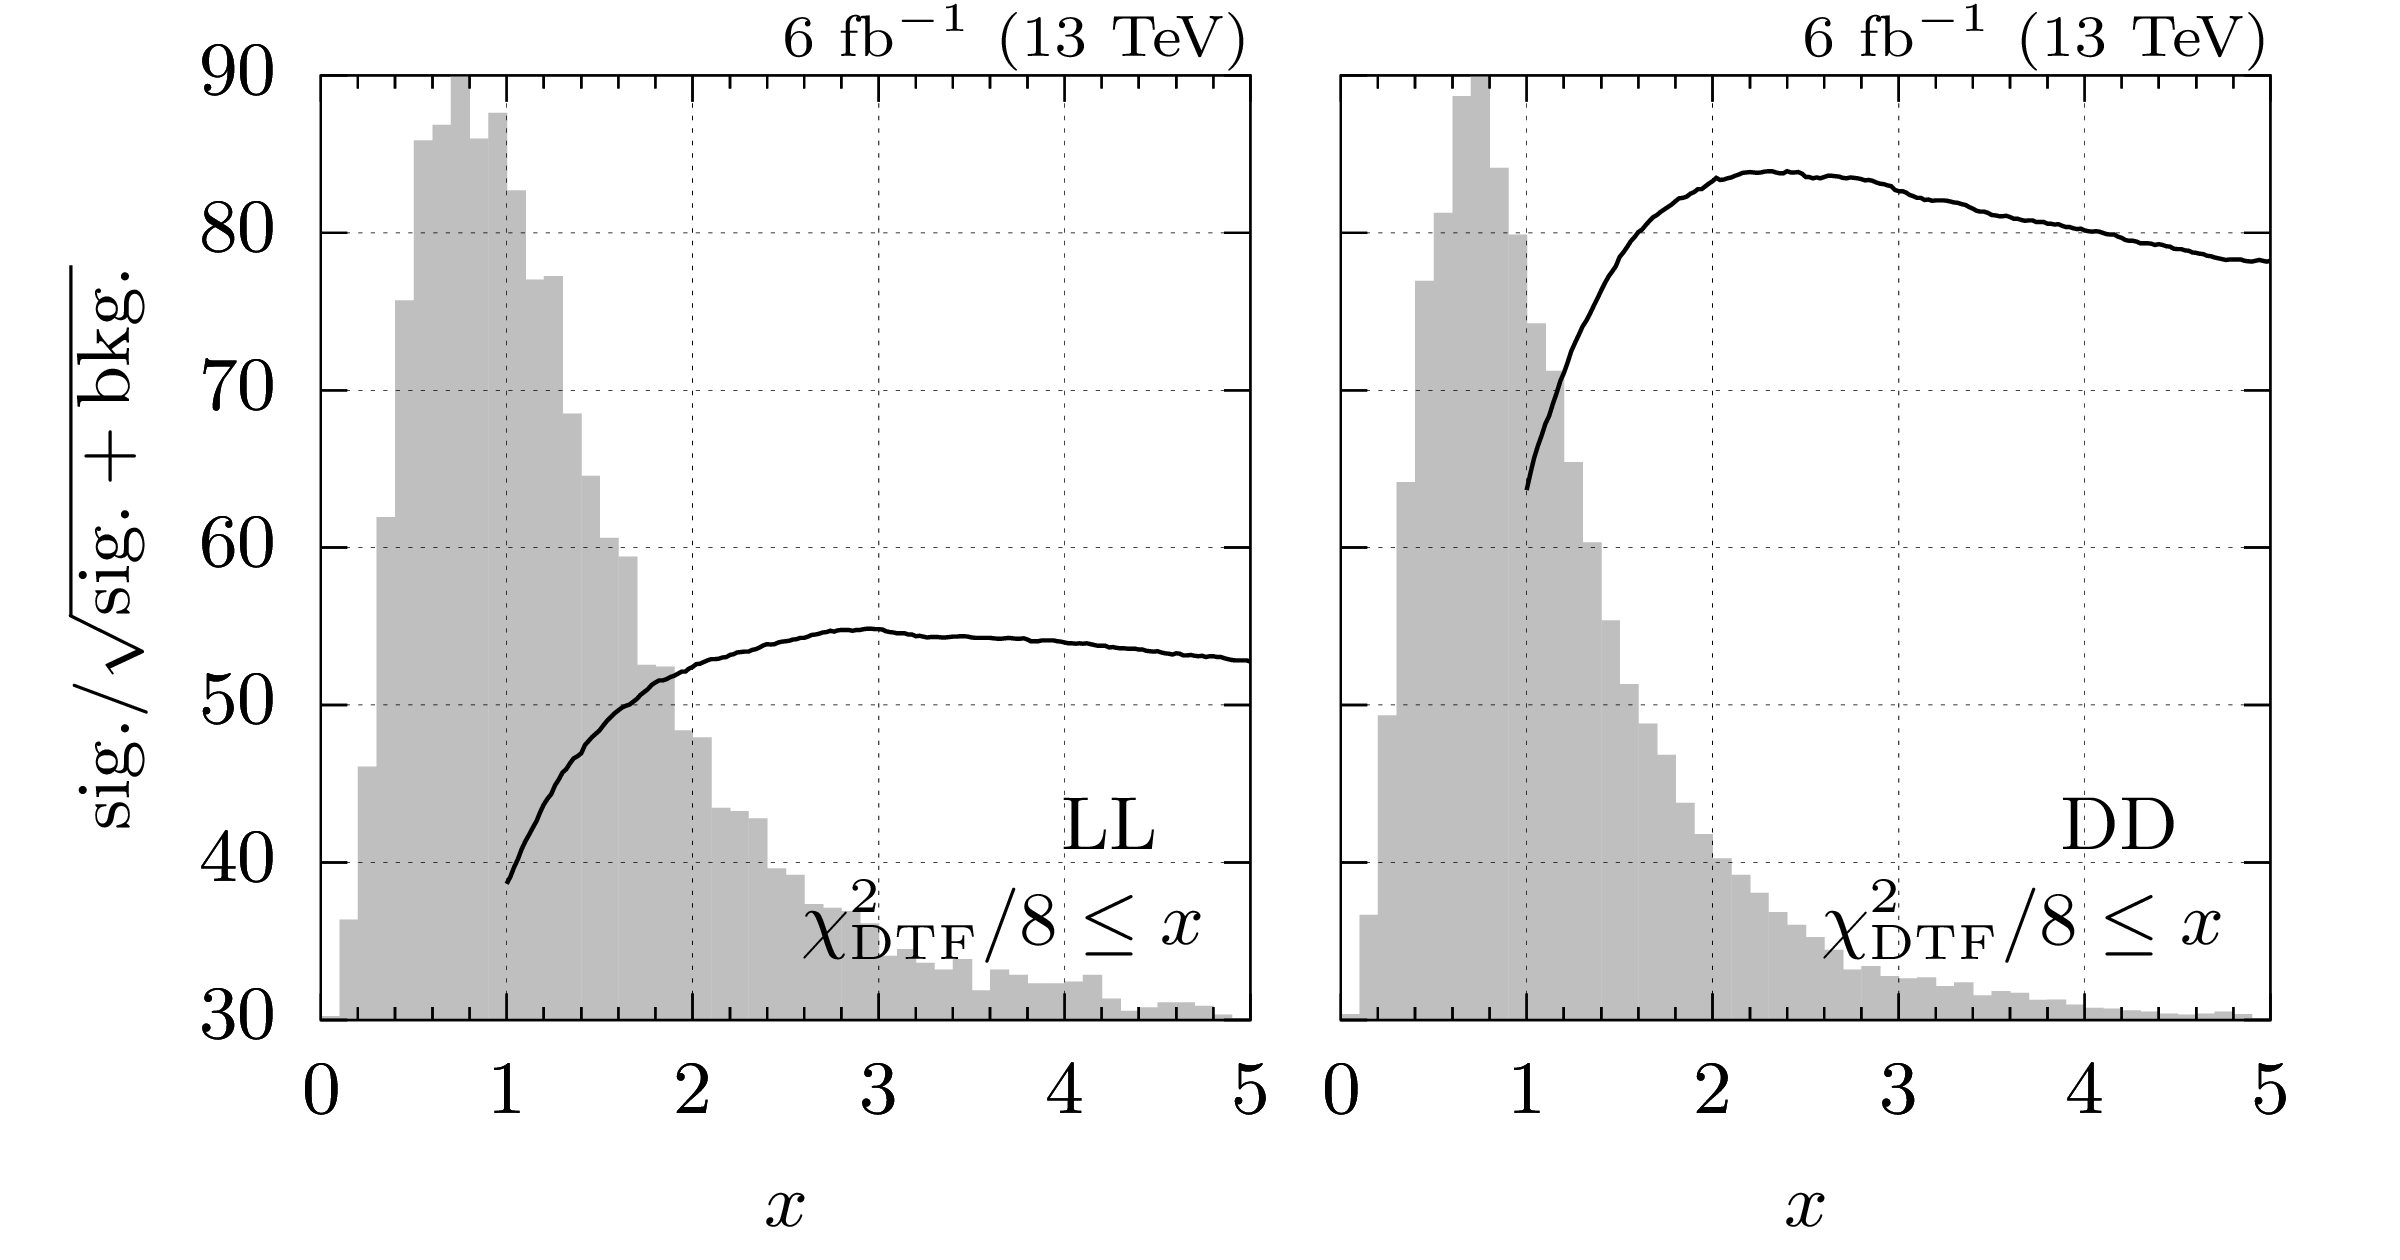
\includegraphics[scale=1.]{Lb2JpsiLz_weighting/sig_chi2.png}
        \caption{\Gls{fom} for veto events if $\chi^2_\text{DTF}/\mathrm{\gls{dof}} > x$.}
    \end{subfigure}
    \par\bigskip 
    \begin{subfigure}{\textwidth}
        \centering 
        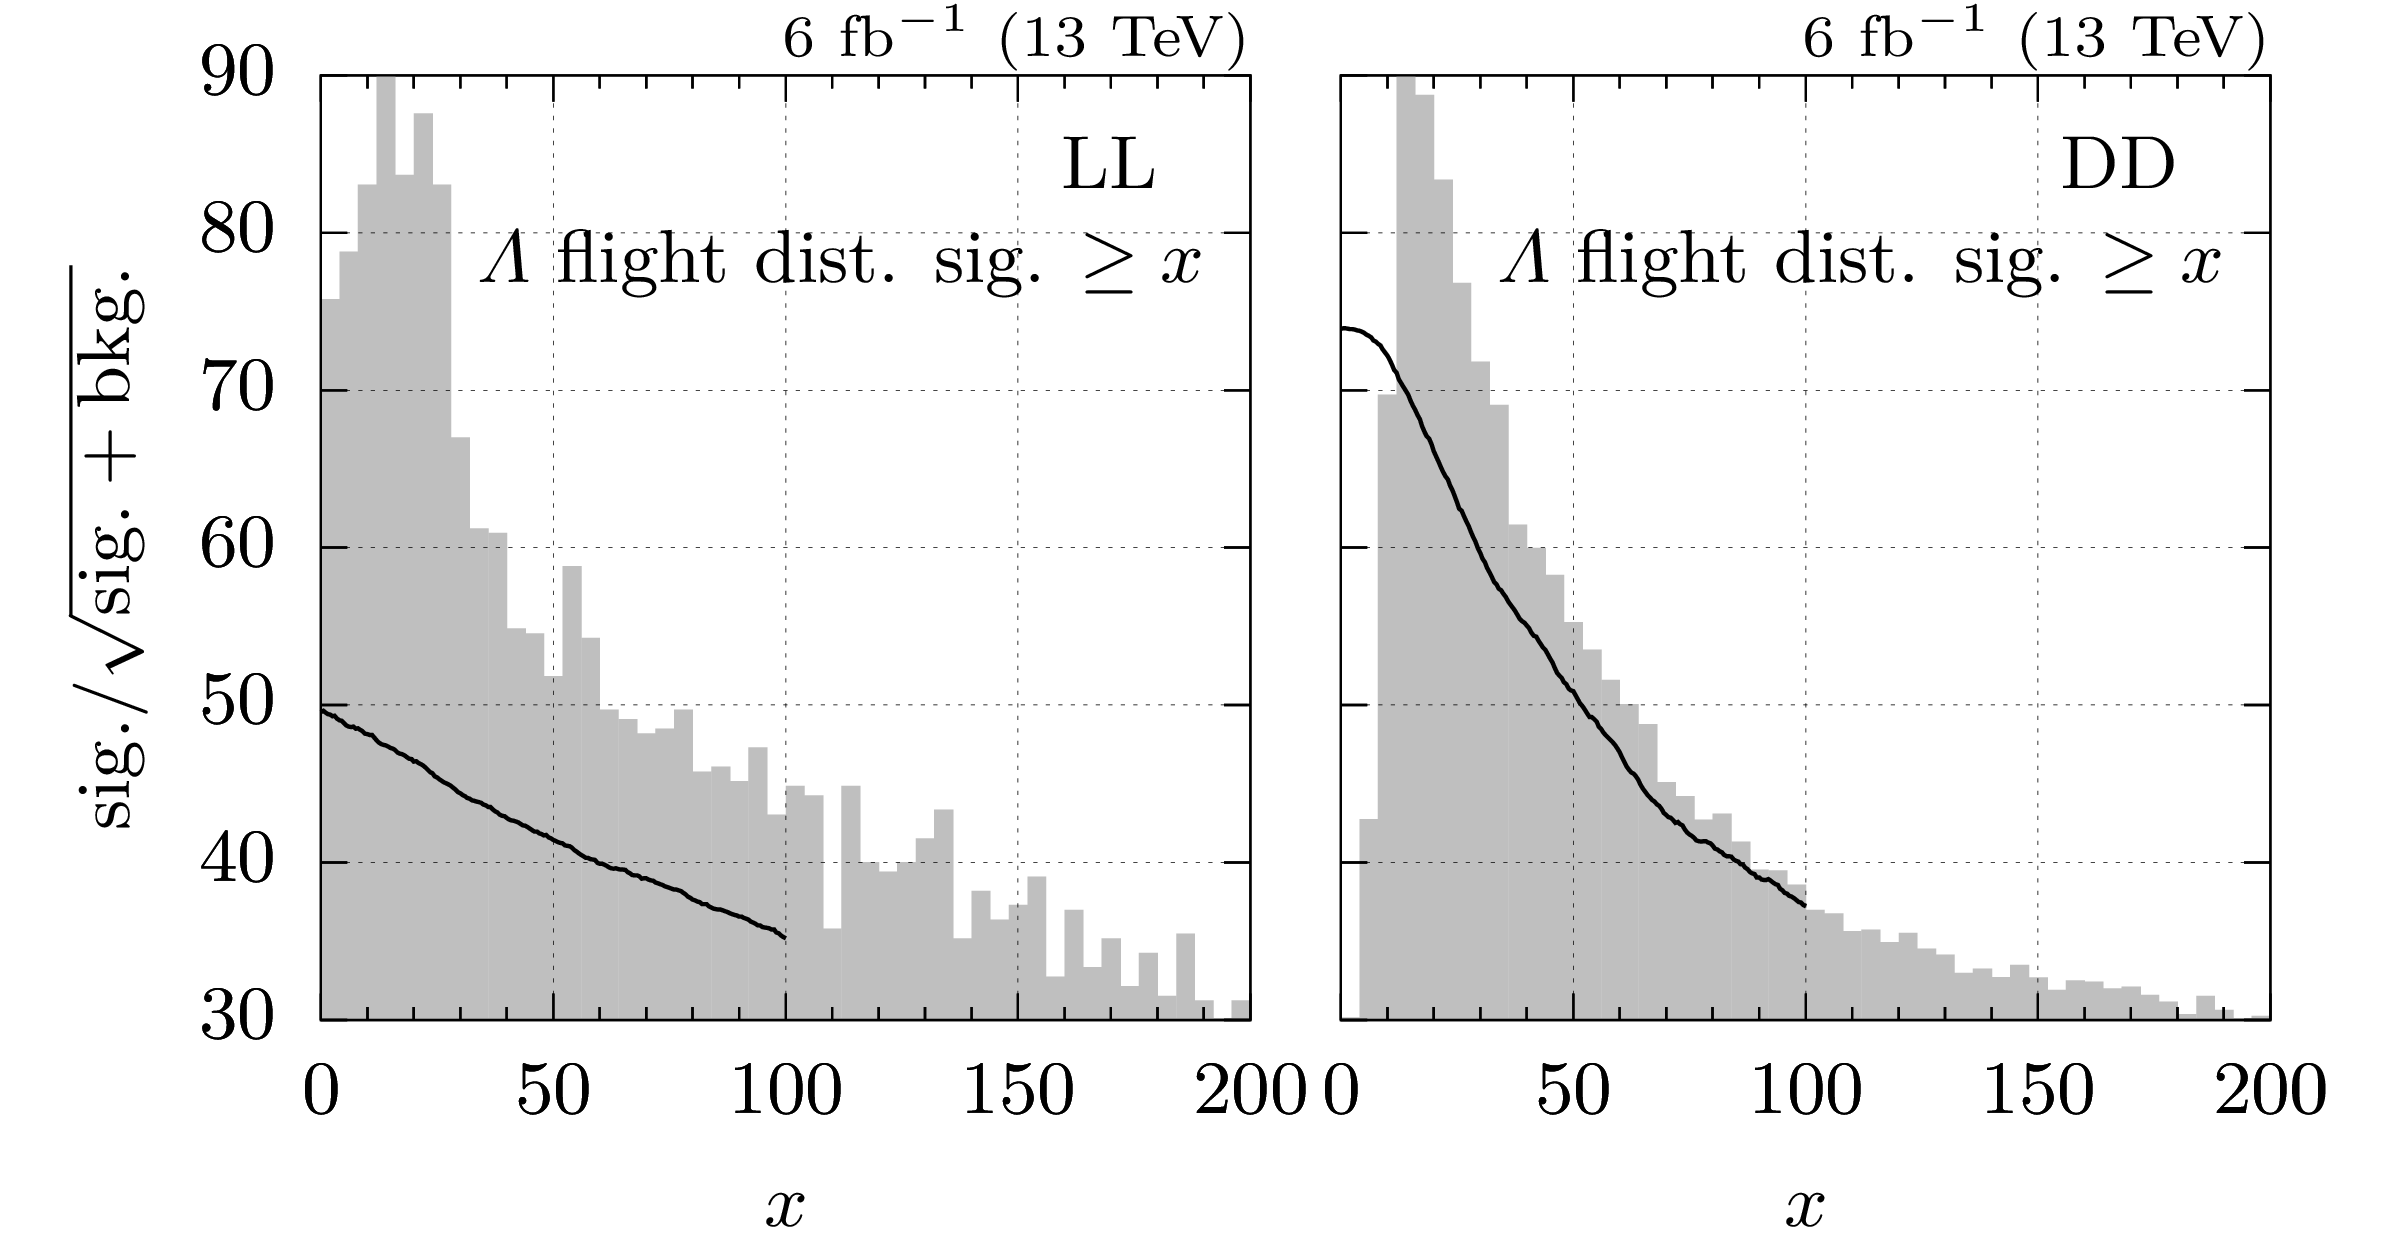
\includegraphics[scale=1.]{Lb2JpsiLz_weighting/sig_LzFDs.png}
        \caption{\Gls{fom} for veto events if \Lz flight distance significance $< x$.}
    \end{subfigure}
    \par\bigskip
    \begin{subfigure}{\textwidth}
        \centering 
        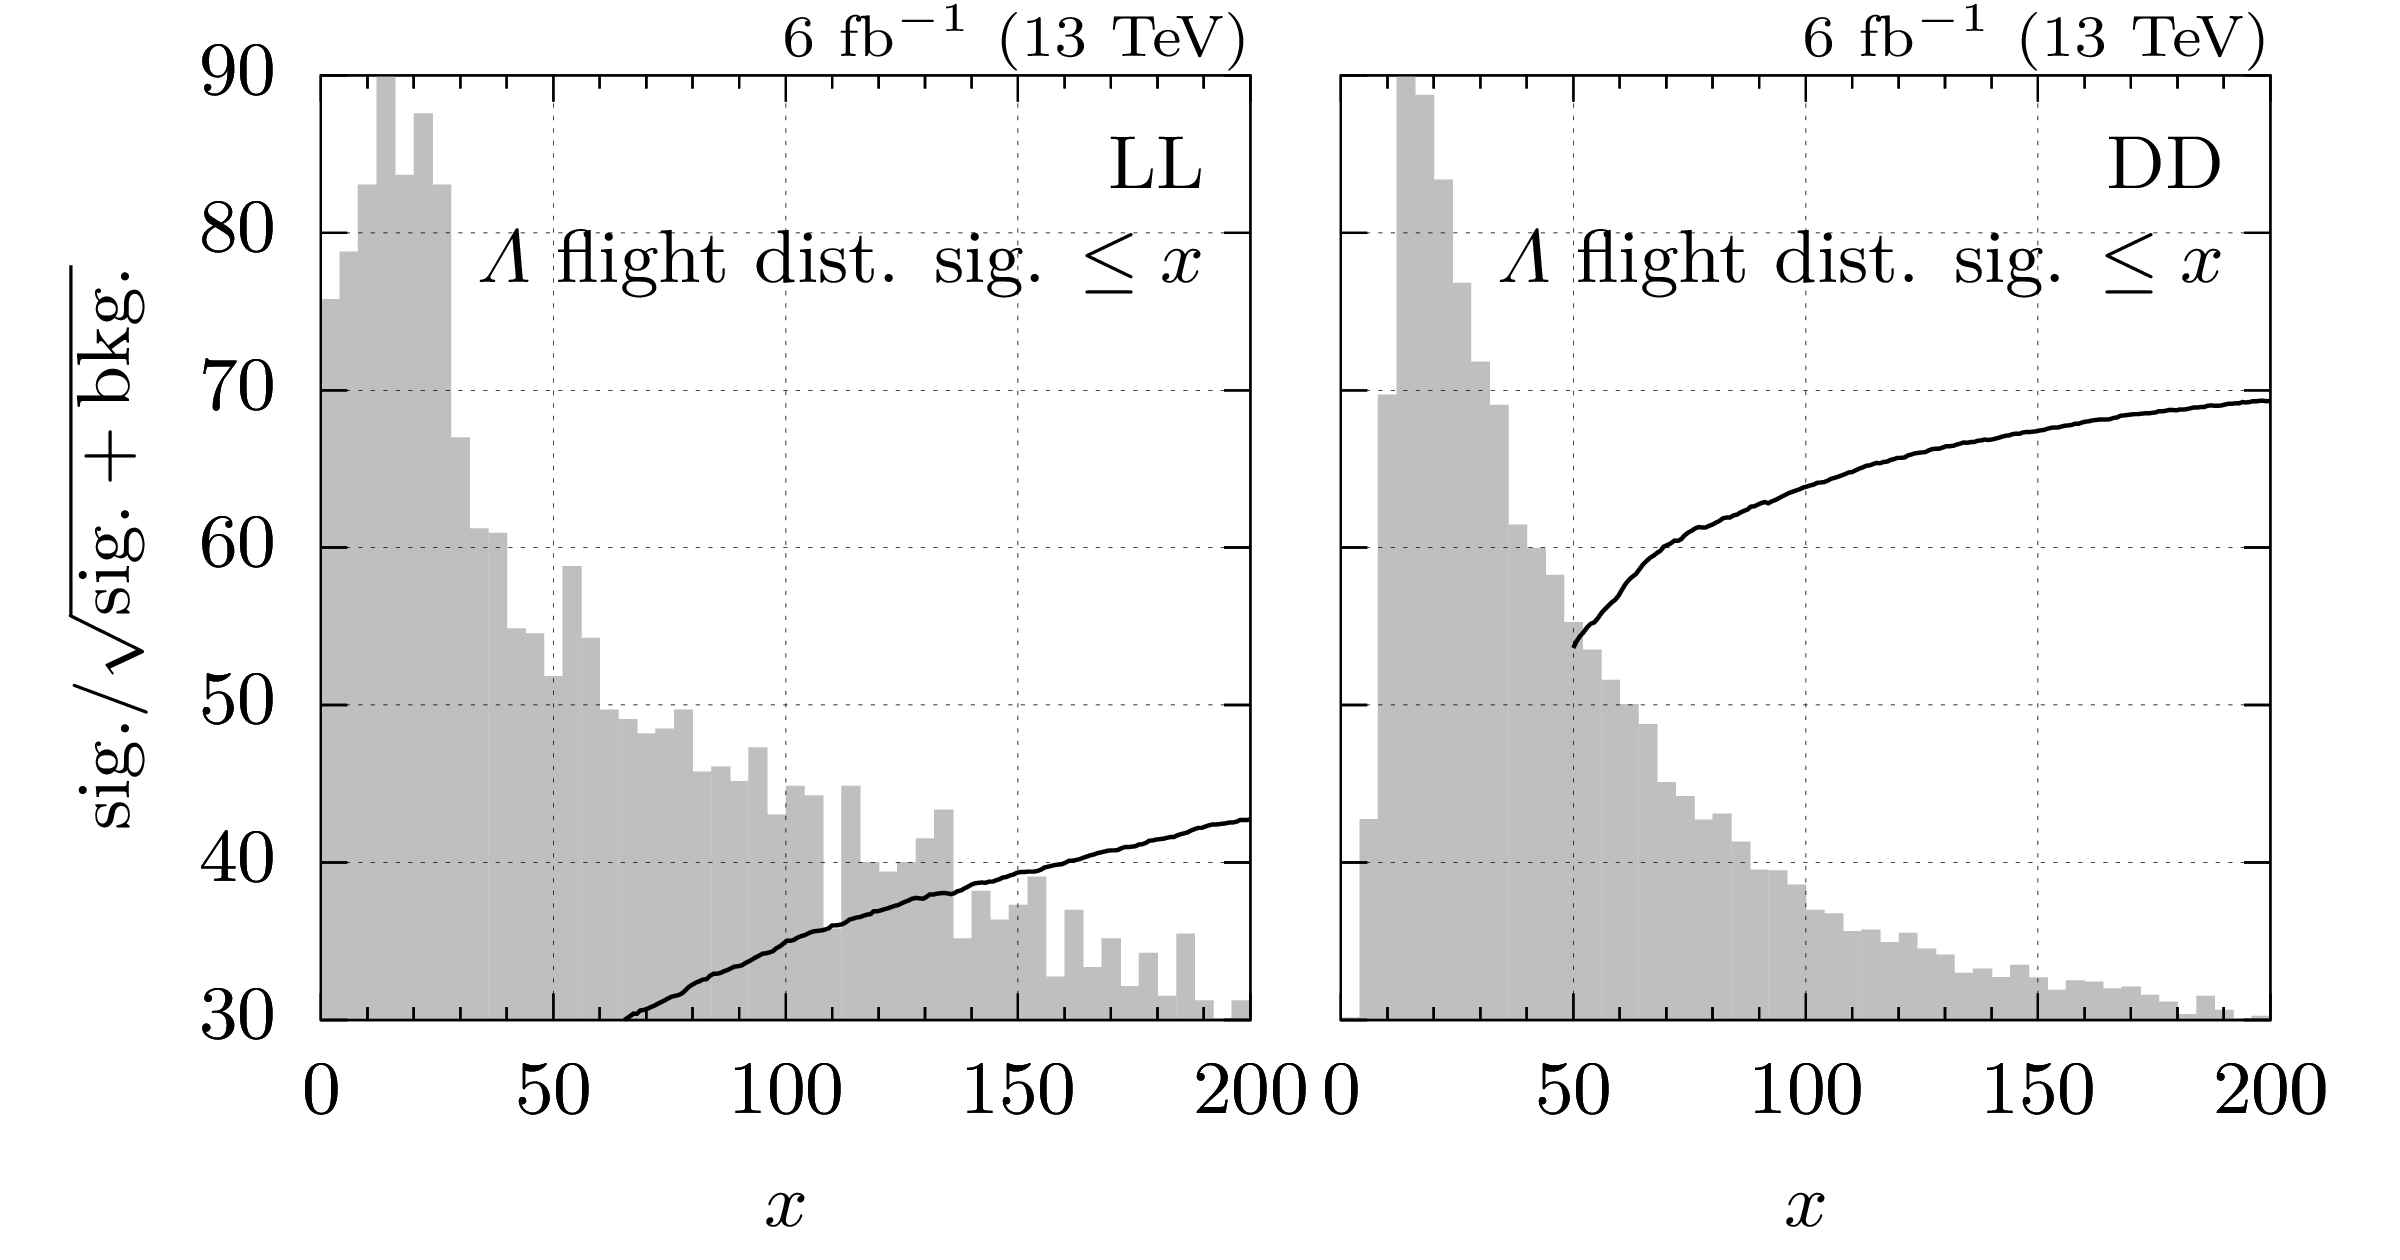
\includegraphics[scale=1.]{Lb2JpsiLz_weighting/isig_LzFDs.png}
        \caption{\Gls{fom} for veto events if \Lz flight distance significance $> x$.}
    \end{subfigure}
    \caption{\Gls{fom} defined as signal efficiency (solid black line) obtained by sideband-subtraction in recorded data and the corresponding distribution of \gls{truthmatched} simulated events (grey shaded area). The \gls{fom} of the \Lz flight distance significance is monotonic for requirements that either prefer large or low values and thus discourage an additional selection w.r.t.\ this feature.}
    \label{fig:LbToJpsiLz_weighting_fom}
\end{figure}
The signal significance for a selection w.r.t.\ $\chi^2_\text{DTF}$ has a maximum for \gls{LL} and \gls{DD} tracks, implying that signal events prefer smaller values of $\chi^2_\text{DTF}$, \ie{}, stronger support for the assumed hypothesis of the \gls{dtf}, and thus motivates the selection criterion for the tight selection
\begin{equation}
    \label{eq:LbToJpsiLz_tightsel}
    \chi^2_\text{DTF} \overset{!}{\le}
    \begin{cases}
        3 & \text{(LL)}, \\
        2 & \text{(DD)},
    \end{cases}
\end{equation}
whereas the \gls{fom} of the \Lz flight distance significance is monotonic for requirements that either prefer large or low values and thus discourage an additional selection w.r.t.\ this feature.
In Fig.~\ref{fig:mLbToJpsiLz_tightsel} we show the invariant mass $m(\jpsi\Lz)$ after applying this and all previously mentioned selection requirements.

\begin{figure}[htbp]
    \centering
    \begin{subfigure}[b]{.49\textwidth}
        \centering
        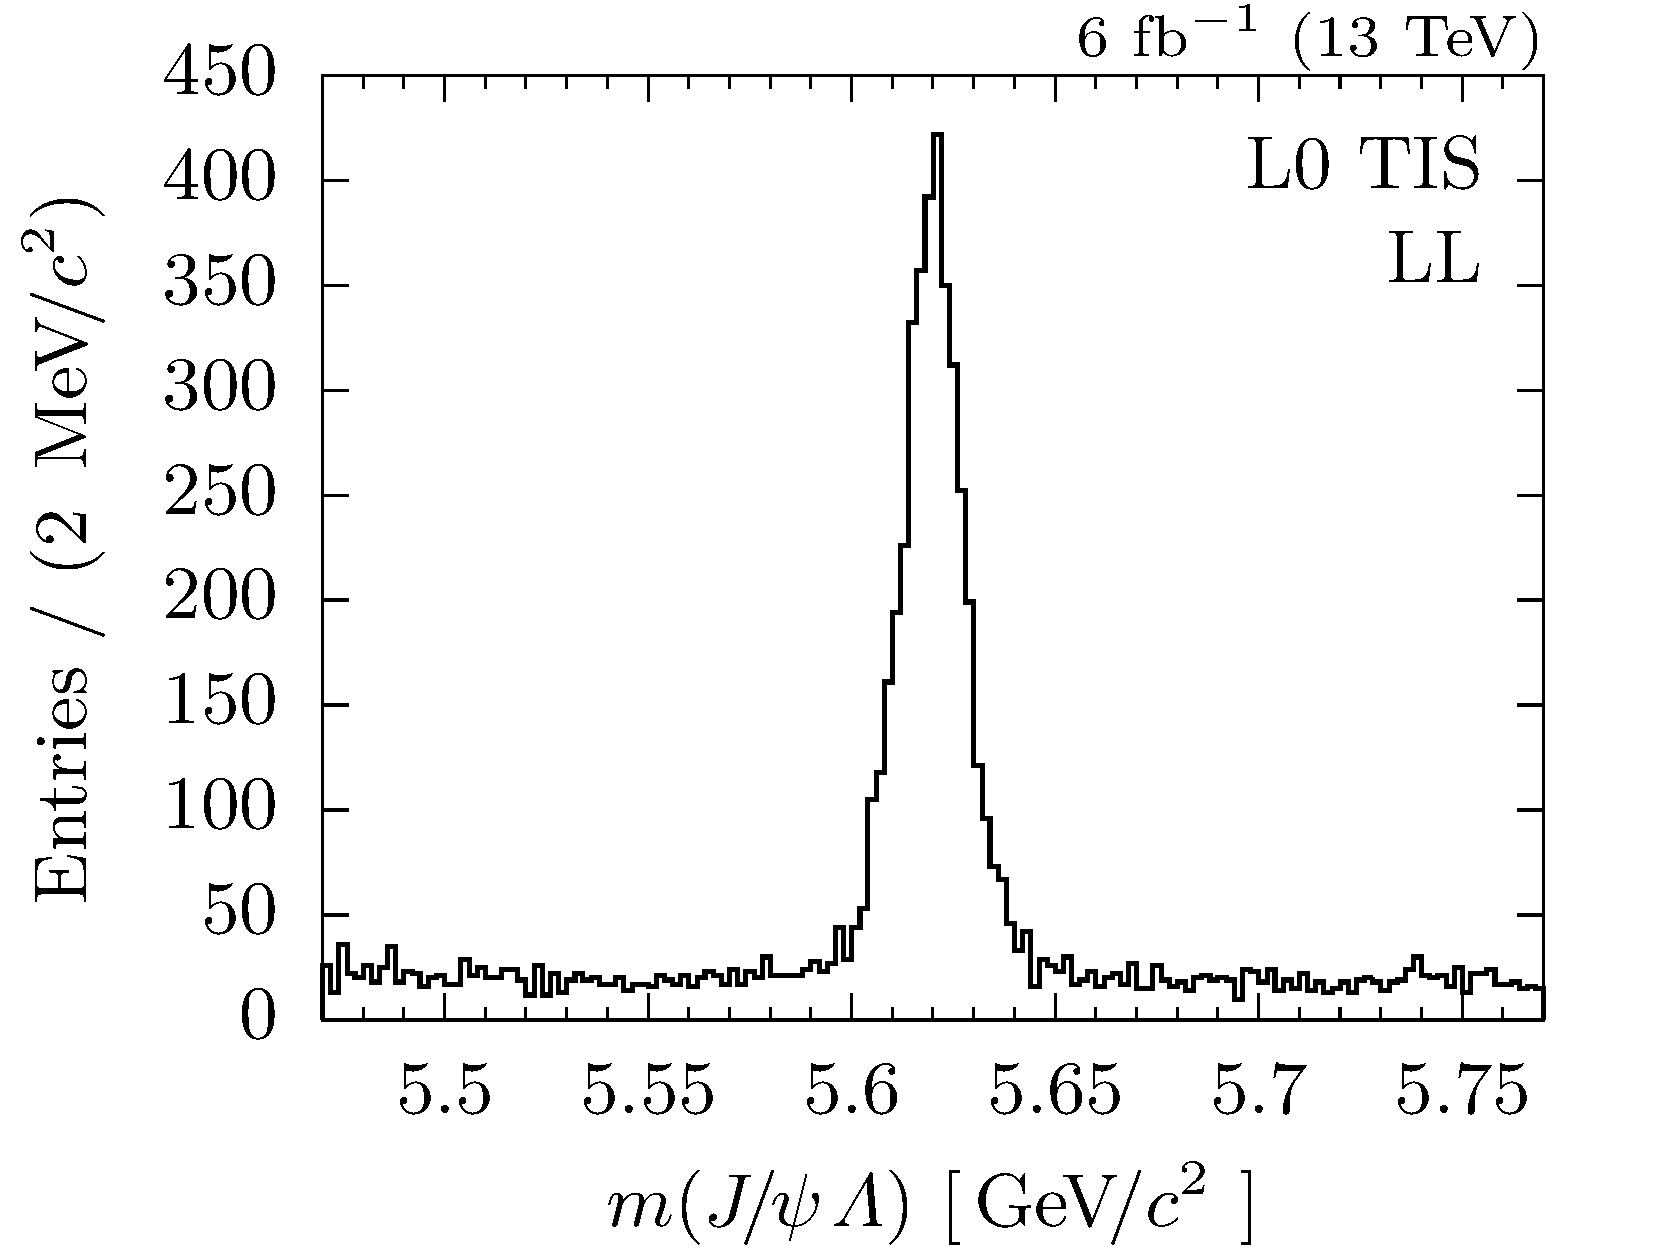
\includegraphics[scale=1.]{Lb2JpsiLz_weighting/hLbM_LL_final.png}
        \caption{\Lz candidates rec.\ from \gls{LL} tracks.}
    \end{subfigure}
    \begin{subfigure}[b]{.49\textwidth}
        \centering
        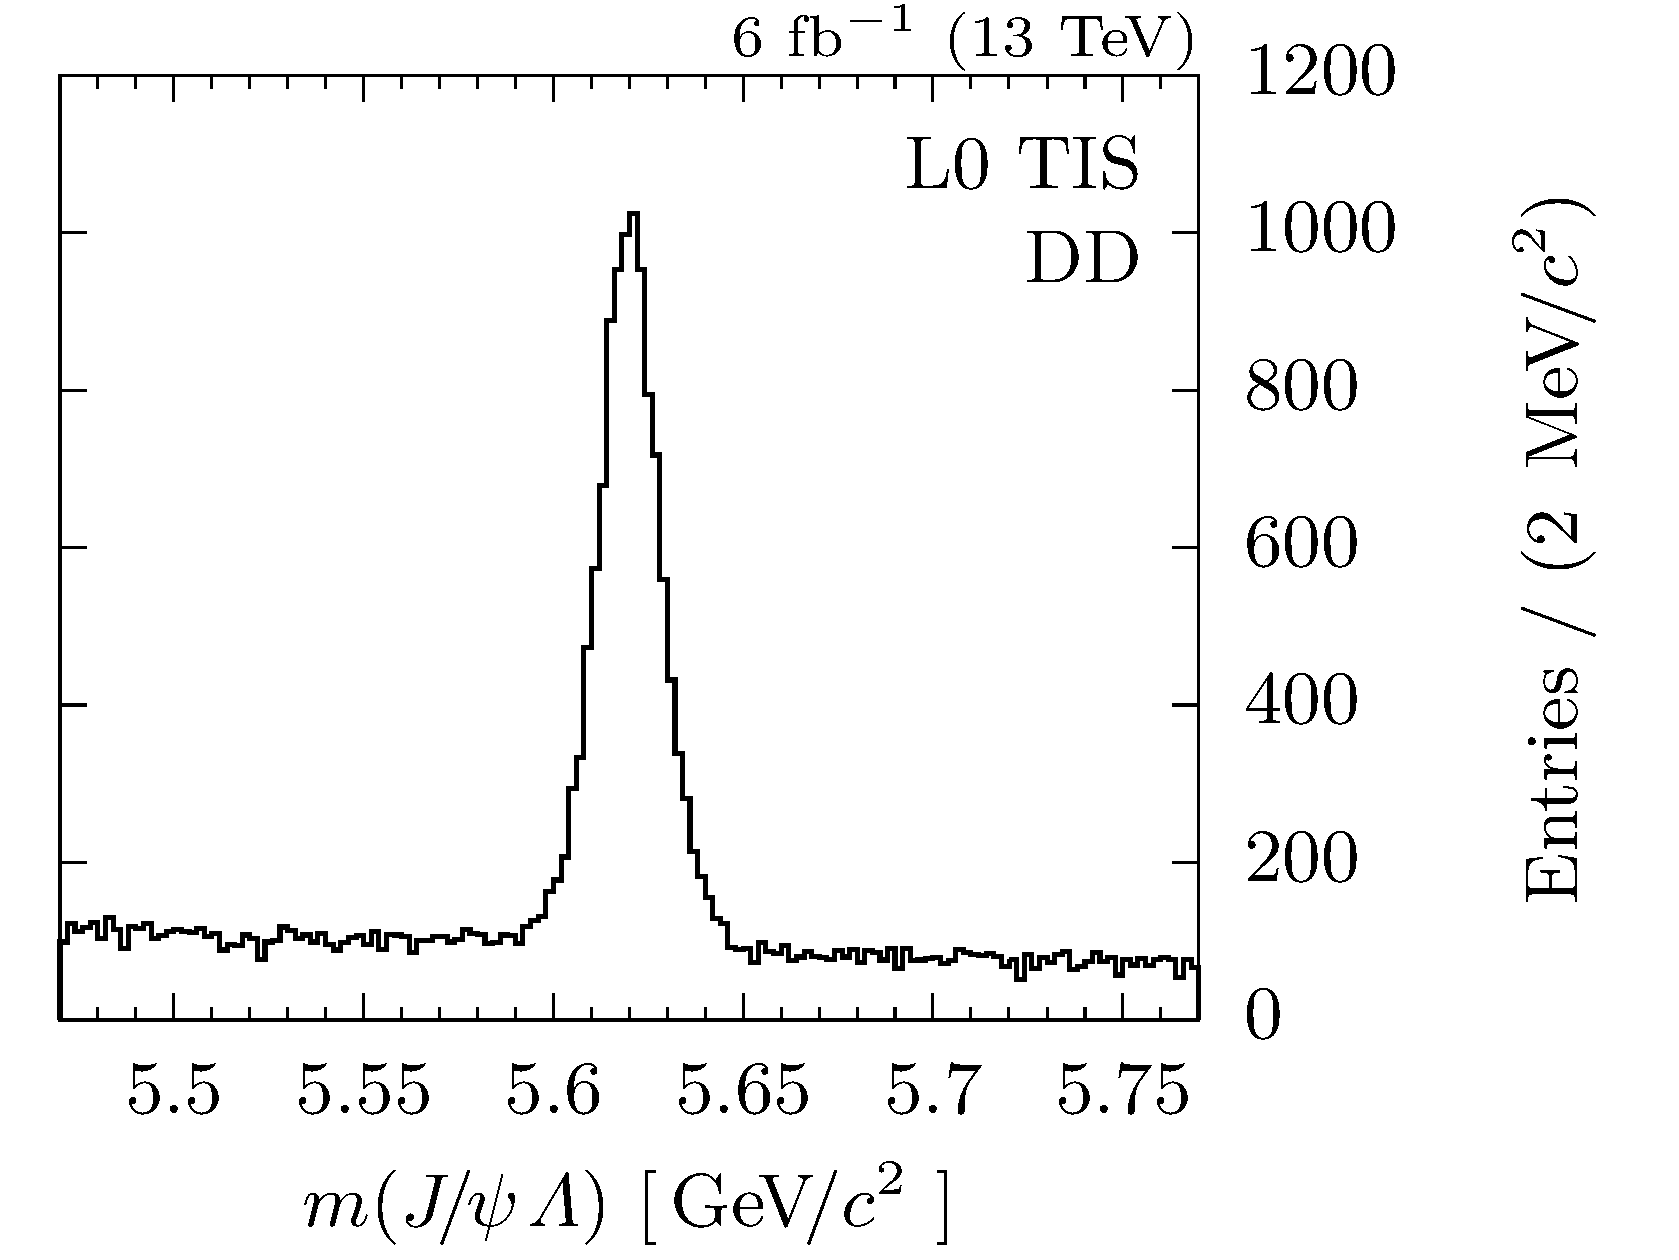
\includegraphics[scale=1.]{Lb2JpsiLz_weighting/hLbM_DD_final.png}
        \caption{\Lz candidates rec.\ from \gls{DD} tracks.}
    \end{subfigure}
    \caption{Combined invariant mass of \jpsi and \Lz candidates after tight selection from recorded data. (Including \gls{lzero} \gls{tis} only requirement.) This selection is used for determining the weights for tuning \gls{mc} simulated \Lb decays.}
    \label{fig:mLbToJpsiLz_tightsel}
\end{figure}

\subsubsection{Efficiency Determination of the Tight Selection}
\label{sec:weights_tightsel}
The technique of sideband subtraction also leverages the estimation of a data driven efficiency determination of the selections given in Eq.~\eqref{eq:LbToJpsiLz_tightsel} by evaluating
\begin{equation*}
    \varepsilon := \frac{n_\text{sig}}{n_\text{sig} + \bar n_\text{sig}} \,,
\end{equation*}
where $n_\text{sig}$ and $\bar n_\text{sig}$ are the amount of signal events that pass the selection and the amount of events that are rejected, respectively.
The uncertainty $u_\varepsilon$ of each of these figures is given by the uncertainty of the mean background ($f \sqrt{n_\text{sideband}} = \sqrt{f n_\text{bkg}}$), the fluctuation of the true background around the mean background in the signal region ($\sqrt{n_\text{bkg}}$) and the fluctuation of the true signal around the mean signal ($\sqrt{n_\text{sig}}$)
\begin{equation*}
    u_\varepsilon = \sqrt{n_\text{sig} + (1 + f) n_\text{bkg}}\,,
\end{equation*}
where $f$ is the scale factor that translates the number of observed background events in the sideband region $n_\text{sideband}$ to the estimated number of background events in the signal region $n_\text{bkg} = f \times n_\text{sideband}$.
The amounts $n_\text{sig}$ and $\bar n_\text{sig}$ are statistically independent, hence the uncertainty of the cut efficiency $\varepsilon$ can be extracted by ordinary error propagation.
In Tab.~\ref{tab:LbToJpsiLz_tighsel_eff} we show $n_\text{sig}$ with its associated uncertainty $\sqrt{(1 + f) n_\text{bkg}}$, as well as the selection efficiencies~$\varepsilon$.

\begin{table}[htbp]
    \centering
    \caption{Total amount of signal events $n_\text{sig}$ after applying the tight selection to recorded \decay{\Lb}{\jpsi\Lz} data, as well as the respective selection efficiency $\varepsilon$.}
    \label{tab:LbToJpsiLz_tighsel_eff}
    \begin{tabular}{ccc}
        \toprule
        & $n_\text{sig}$ & $\varepsilon$ \\
        \midrule
        \gls{LL} & $\num{3653} \pm 33$ & $(91.4 \pm 1.2) \,\%$ \\
        \gls{DD} & $\num{9590} \pm 70$ & $(79.1 \pm 0.9) \,\%$ \\
        \bottomrule
    \end{tabular}
\end{table}

\section{Extraction of Weights}
The features transverse momentum $\pt(\Lb)$ and pseudorapidity $\eta(\Lb)$ of the \Lb are not uncorrelated, but related via the identity relation
\begin{equation*}
    \eta = \operatorname{artanh} \frac{p_z}{p} = \operatorname{artanh} \sqrt{1 - \left( \frac{\pt}{p} \right)^2} \,,
\end{equation*}
where $\operatorname{artanh}$ is the inverse hyperbolic tangent (aka area hyperbolic tangent), and $p_z$ and $p$ the $z$-component and magnitude of the momentum, respectively.

%\begin{figure}[htbp]
%    \centering
%    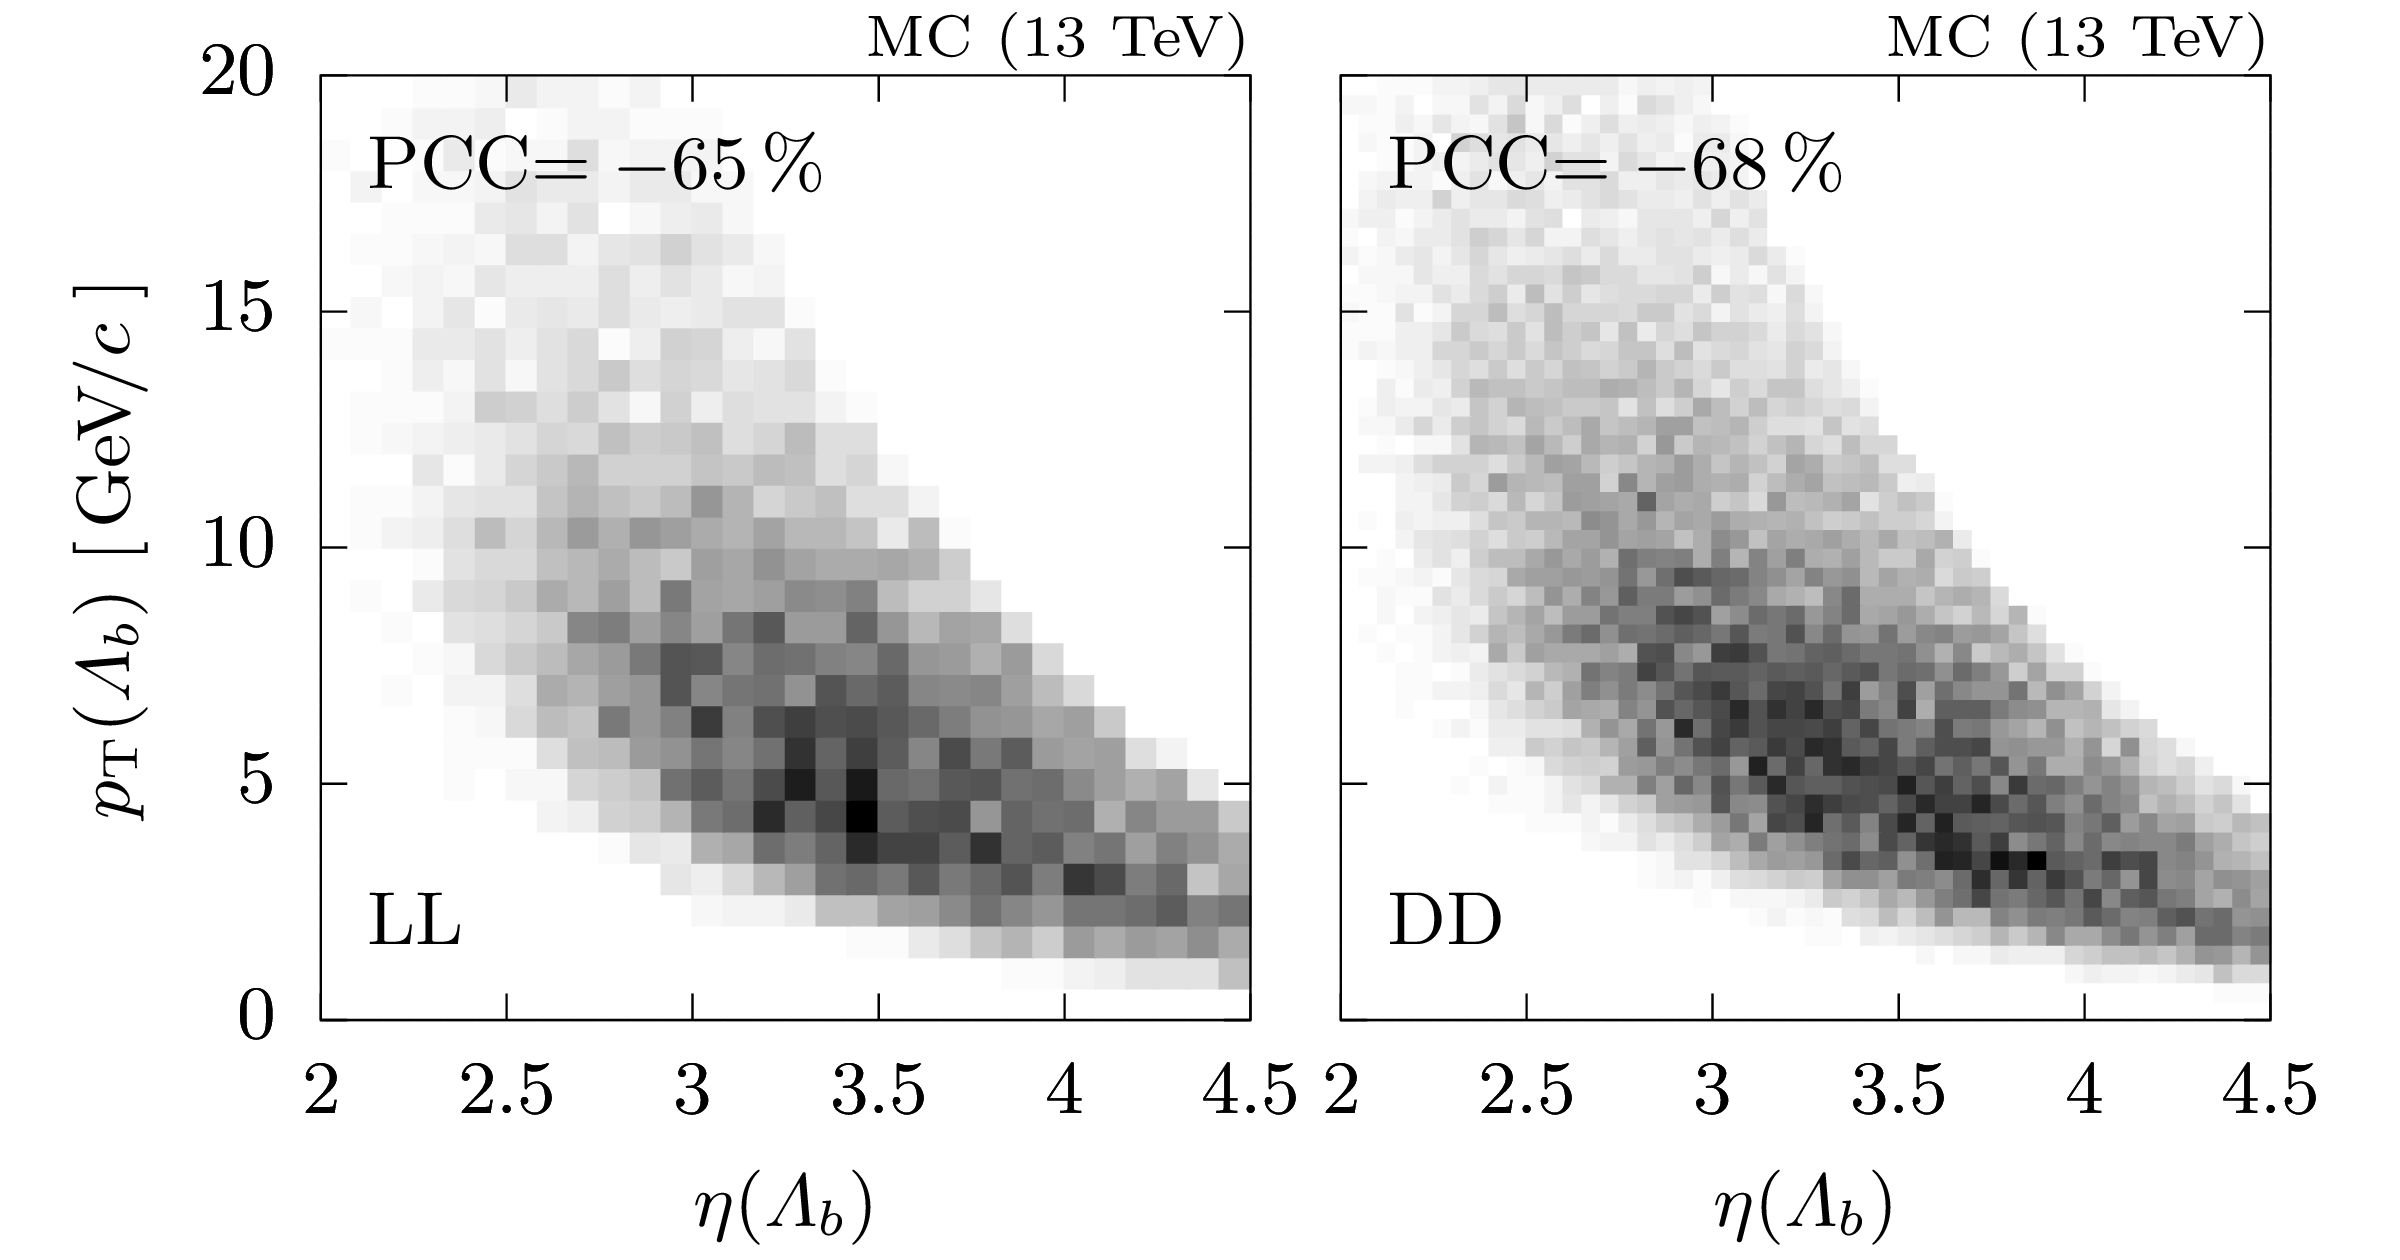
\includegraphics[scale=1.]{Lb2JpsiLz_weighting/corr_eta_pT.png}
%    \caption{Correlation between $\pt(\Lb)$ and $\eta(\Lb)$, as well as the corresponding \gls{pcc} values for \gls{LL} (left) and \gls{DD} tracks (right), estimated for \gls{truthmatched} MC simulated \decay{\Lb}{\jpsi\Lz} events.}
%    \label{fig:corr_eta_pT_LbToJpsiLz}
%\end{figure}
%
%In Fig.~\ref{fig:corr_eta_pT_LbToJpsiLz} we show the correlation between $\pt(\Lb)$ and $\eta(\Lb)$, as well as the corresponding \gls{pcc} values for \gls{LL} (left) and \gls{DD} tracks (right), estimated for \gls{truthmatched} MC simulated \decay{\Lb}{\jpsi\Lz} events.
%The correlation is approximately $-65\,\%$ and $-68\,\%$ for \gls{LL} and \gls{DD} tracks, respectively.
Due to this non-negligible correlation, altering one distribution will also affect the other and vice versa.
Ideally, the extraction of weight factors should be performed in the 2d-plane of both variables.
Reliable weights, though, also require decent statistics which turned out to be problematic, especially for \gls{LL} tracks.

We try two different schemes for extracting weights.
First, we only consider the respective marginal distributions and find the weights in an iterative approach.
The underlying assumption is a factorization of the weights in the 2d-plane $w(\pt, \eta) = w_1(\pt) \times w_2(\eta)$ and thus, per definition, ignores all correlation contributions.
We cross-check this assumption with a third quantity $p(\Lb)$ which is another marginal distribution in the $\pt$-$\eta$ space.

In this first scheme we discover unexpected deviations between the distributions of $\eta(\Lb)$ for different track types but at the same time a decent compatibility with one for all $\eta(\Lb)$ weights w.r.t.\ the given statistical uncertainties.
This motivates our second scheme where weights are extracted based on $\pt(\Lb)$ only.

\subsection{Truth Matched vs. Sideband Subtracted MC Simulated Events}
\label{sec:LbToJpsiLz_tm_vs_ss}

Similar to recorded data, \gls{mc} simulated events contain not only signal, but also background events coming either from true physical background processes or are combinatoric remnants.
A marked difference between recorded and simulated events is that the latter could be attached with a label and thus, in theory, can be unambiguously identified as signal (\gls{truthmatched}) or background event (\textit{unmatched}).
However, in practice this approach suffers from a non-zero mistag probability during reconstruction which introduces an unphysical error.
This error has no counter part in recorded data which is critical when correlated with the variables that are the objective of the weighting scheme.

\begin{figure}[htbp]
    \centering
    \begin{subfigure}{\textwidth}
        \centering
        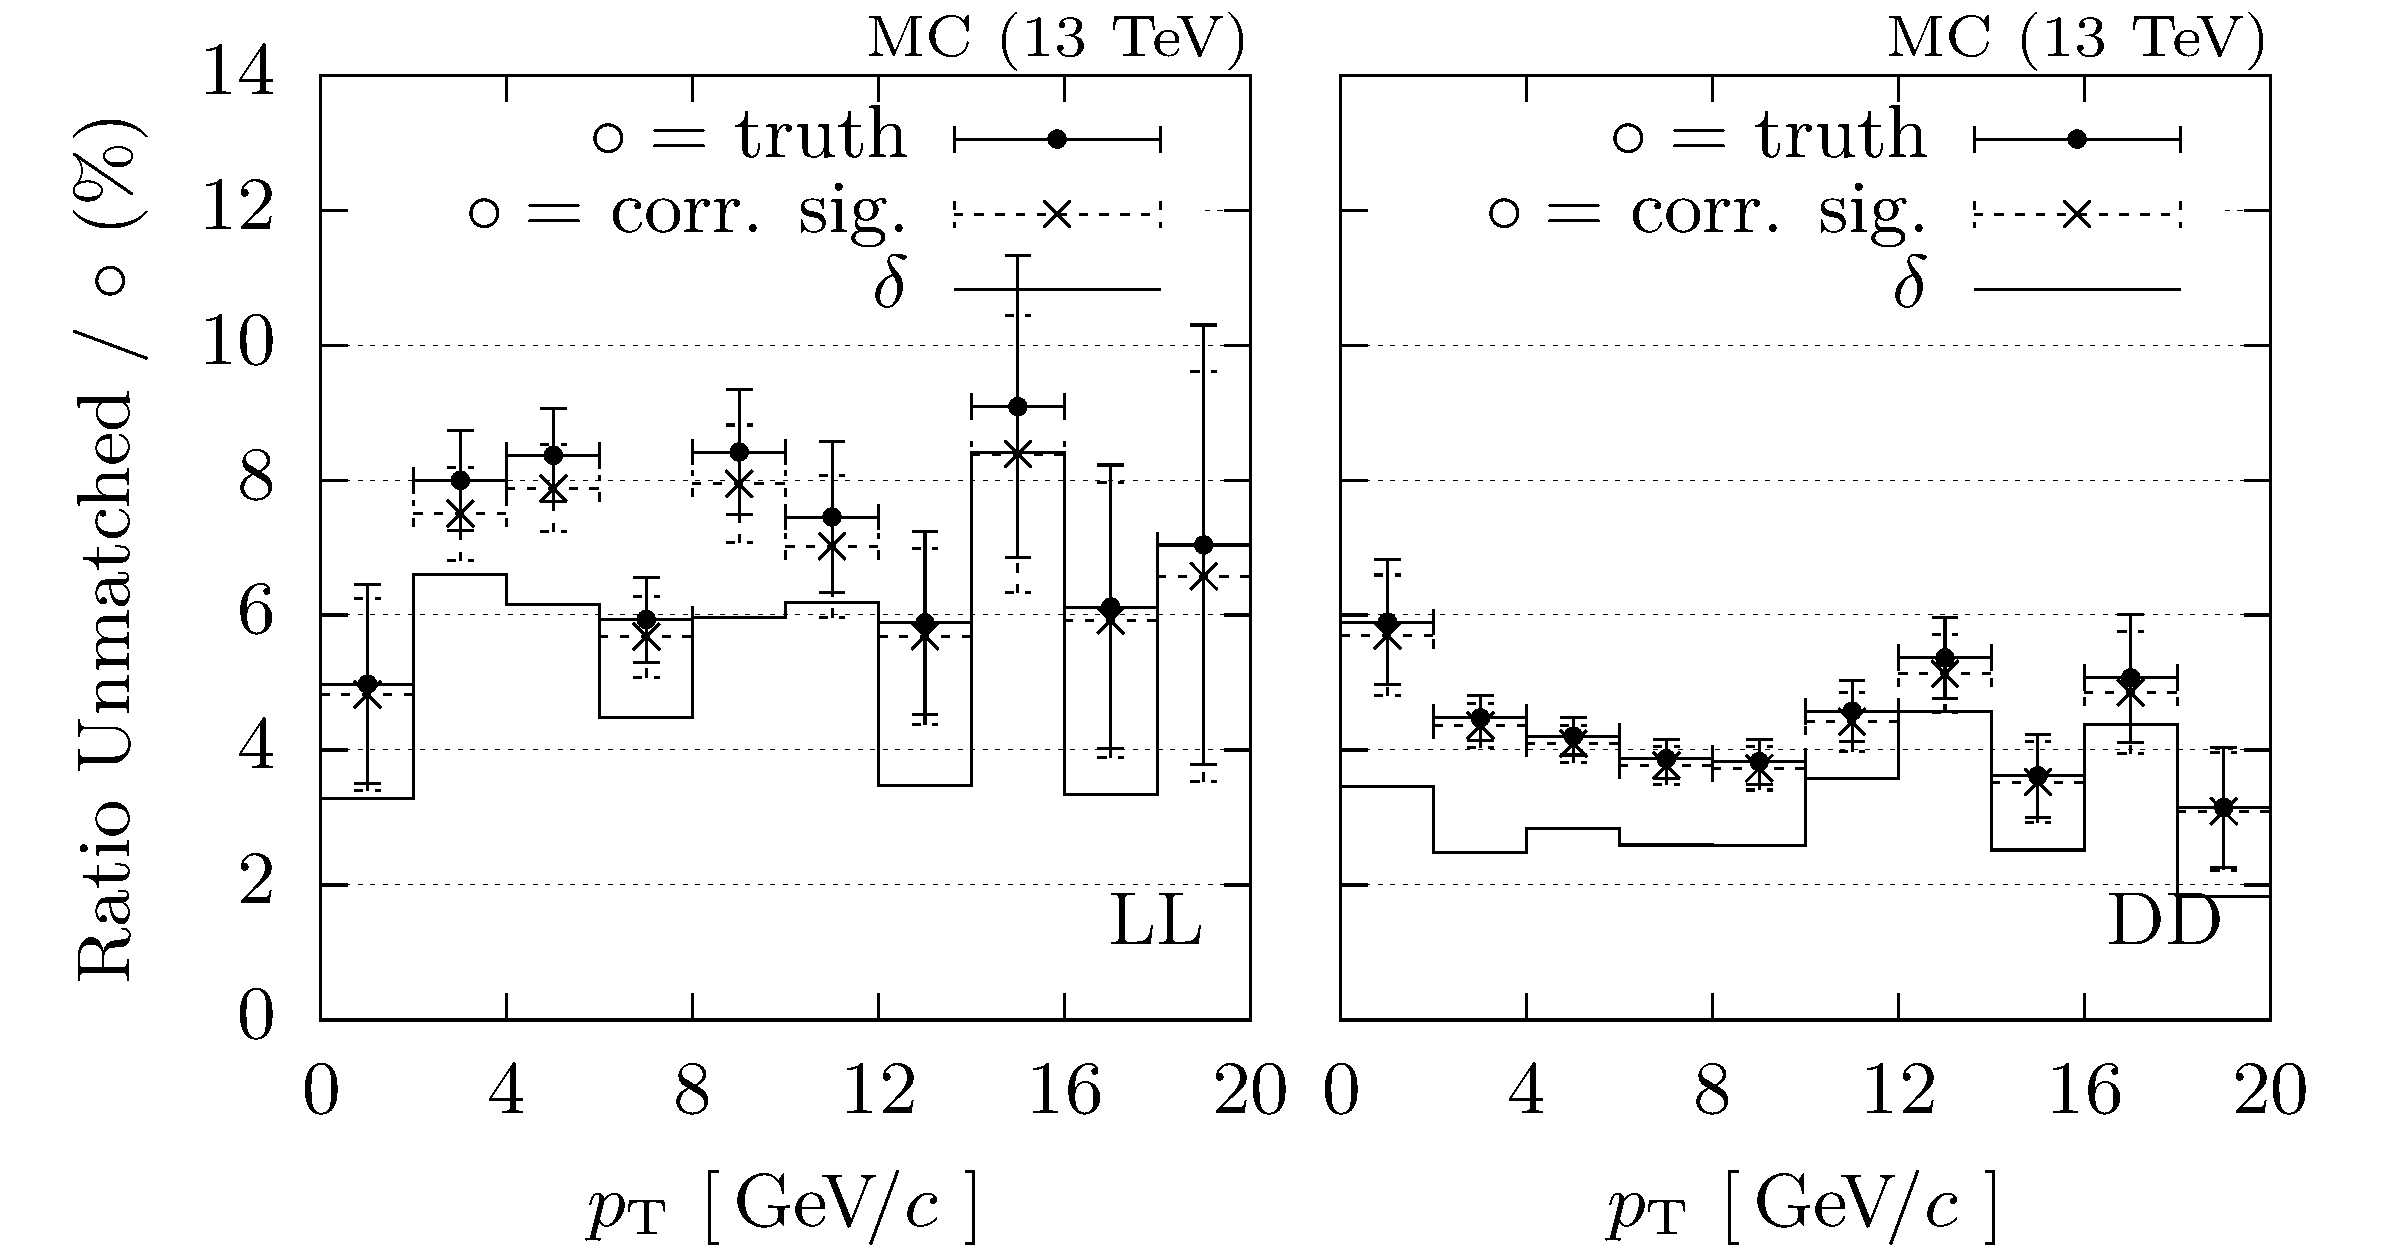
\includegraphics[scale=1.]{Lb2JpsiLz_weighting/htmratio_pT.png}
    \end{subfigure}
    \par\bigskip 
    \begin{subfigure}{\textwidth}
        \centering
        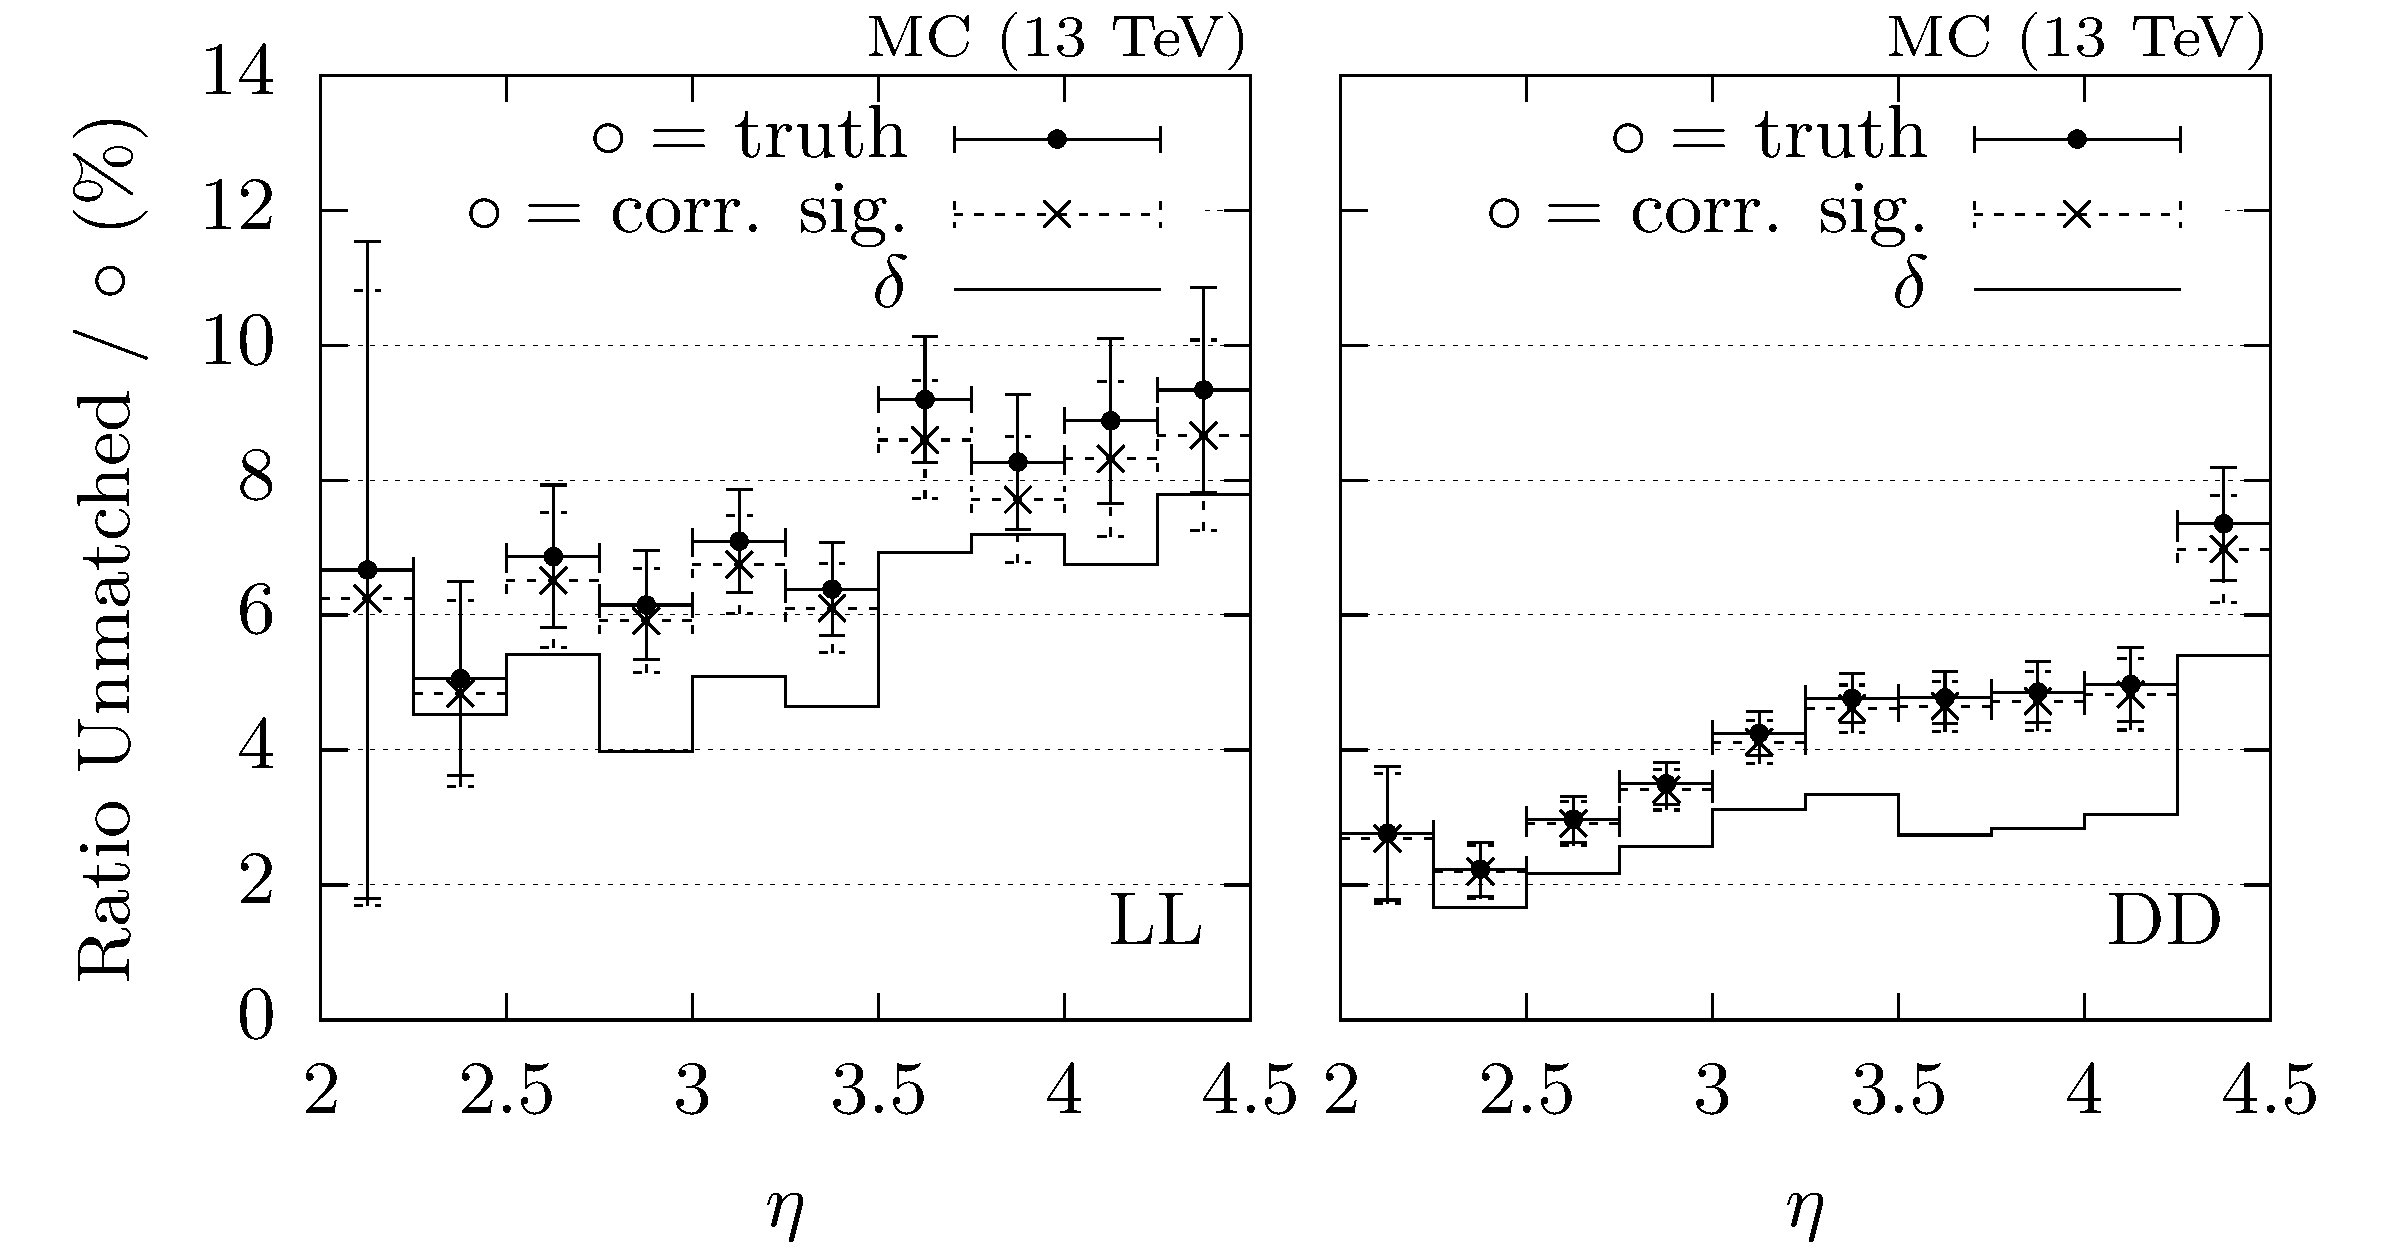
\includegraphics[scale=1.]{Lb2JpsiLz_weighting/htmratio_eta.png}
    \end{subfigure}
    \caption{Comparison of the ratio of unmatched and \gls{truthmatched} (referred to as \textit{truth}) with the ratio of unmatched and sideband corrected events (referred to as \textit{corr. sig.}) in bins of $\pt(\Lb)$ (top) and $\eta(\Lb)$ (bottom) for track types \gls{LL} (left) and \gls{DD} (right). The values of $\delta$, as defined in Eq.~\eqref{eq:weightdelta}, are shown at the same $y$-axis. The given error bars do not account for the strong correlations between unmatched and \gls{truthmatched} events.}
    \label{fig:htmratio_LbToJpsiLz}
\end{figure}

In the Fig.~\ref{fig:htmratio_LbToJpsiLz} we compare the ratio of unmatched and \gls{truthmatched} events with the ratio of unmatched and sideband corrected events as a function of $\pt(\Lb)$ and $\eta(\Lb)$.
The samples used for determining the ratios are pairwise uncorrelated, whereas the ratios themselves are strongly correlated which has to be taken into account when comparing the distribution of the ratios.
We define $\delta$ as the correction when using \gls{truthmatched} events during the weighting procedure instead of sideband corrected simulated events,
\begin{equation}
    \label{eq:weightdelta}
    1 + \delta := \frac{b'}{b} = 1 + \frac{\Delta}{a/b'} \,,
\end{equation}
where $a$, $b$ and $b'$ are the amount of unmatched, \gls{truthmatched} and sideband corrected simulated events, respectively and $\Delta$ is defined as the difference
\begin{equation*}
    \Delta := \frac{a}{b} - \frac{a}{b'} \,.
\end{equation*}
We note that in the limit of empty sidebands $b' = b+a$ and thus $\delta = a/b$, as expected.
From Fig.~\ref{fig:htmratio_LbToJpsiLz} we infer $\mathcal{O}(\delta) = 5\,\%$.
Non uniform contributions of $\delta$ will skew the distributions of the weights.
Further, if $\delta$ is correlated differently for \gls{LL} and \gls{DD}, this introduces an unphysical difference between the track types.
(An absolute difference of $\delta$ introduces a uniformly distributed difference and is thus less critical.)
From these figures, such a correlation cannot be excluded with high confidence and we will therefore not use \gls{truthmatched}, but sideband corrected \gls{mc} simulated events for the weighting process.

\subsection{Scheme 1}
\label{sec:LbToJpsiLz_w1}

In this first scheme we extract weights by iteratively improving the $\pt(\Lb)$ and $\eta(\Lb)$ dependent weight $w$,
\begin{equation*}
    w(\pt, \eta) = w_1(\pt) \times w_2(\eta) \,,
\end{equation*}
and validate its values in the $p(\Lb)$ distribution. 

In Fig.~\ref{fig:LbToJpsiLz_hpT_corr} and Fig.~\ref{fig:LbToJpsiLz_heta_corr} we show the distributions of $\pt(\Lb)$ and $\eta(\Lb)$ for recorded data, as well as for simulated events as obtained from sideband subtractions.
These distributions are used pairwise to get the binned ratio of recorded data and simulated events for each of these features as shown in Fig.~\ref{fig:LbToJpsiLz_hratio}, where each bin corresponds to the ratio of the respective bin in the histogram of reconstructed and \gls{mc} simulated data.

\begin{figure}[htbp]
    \centering
    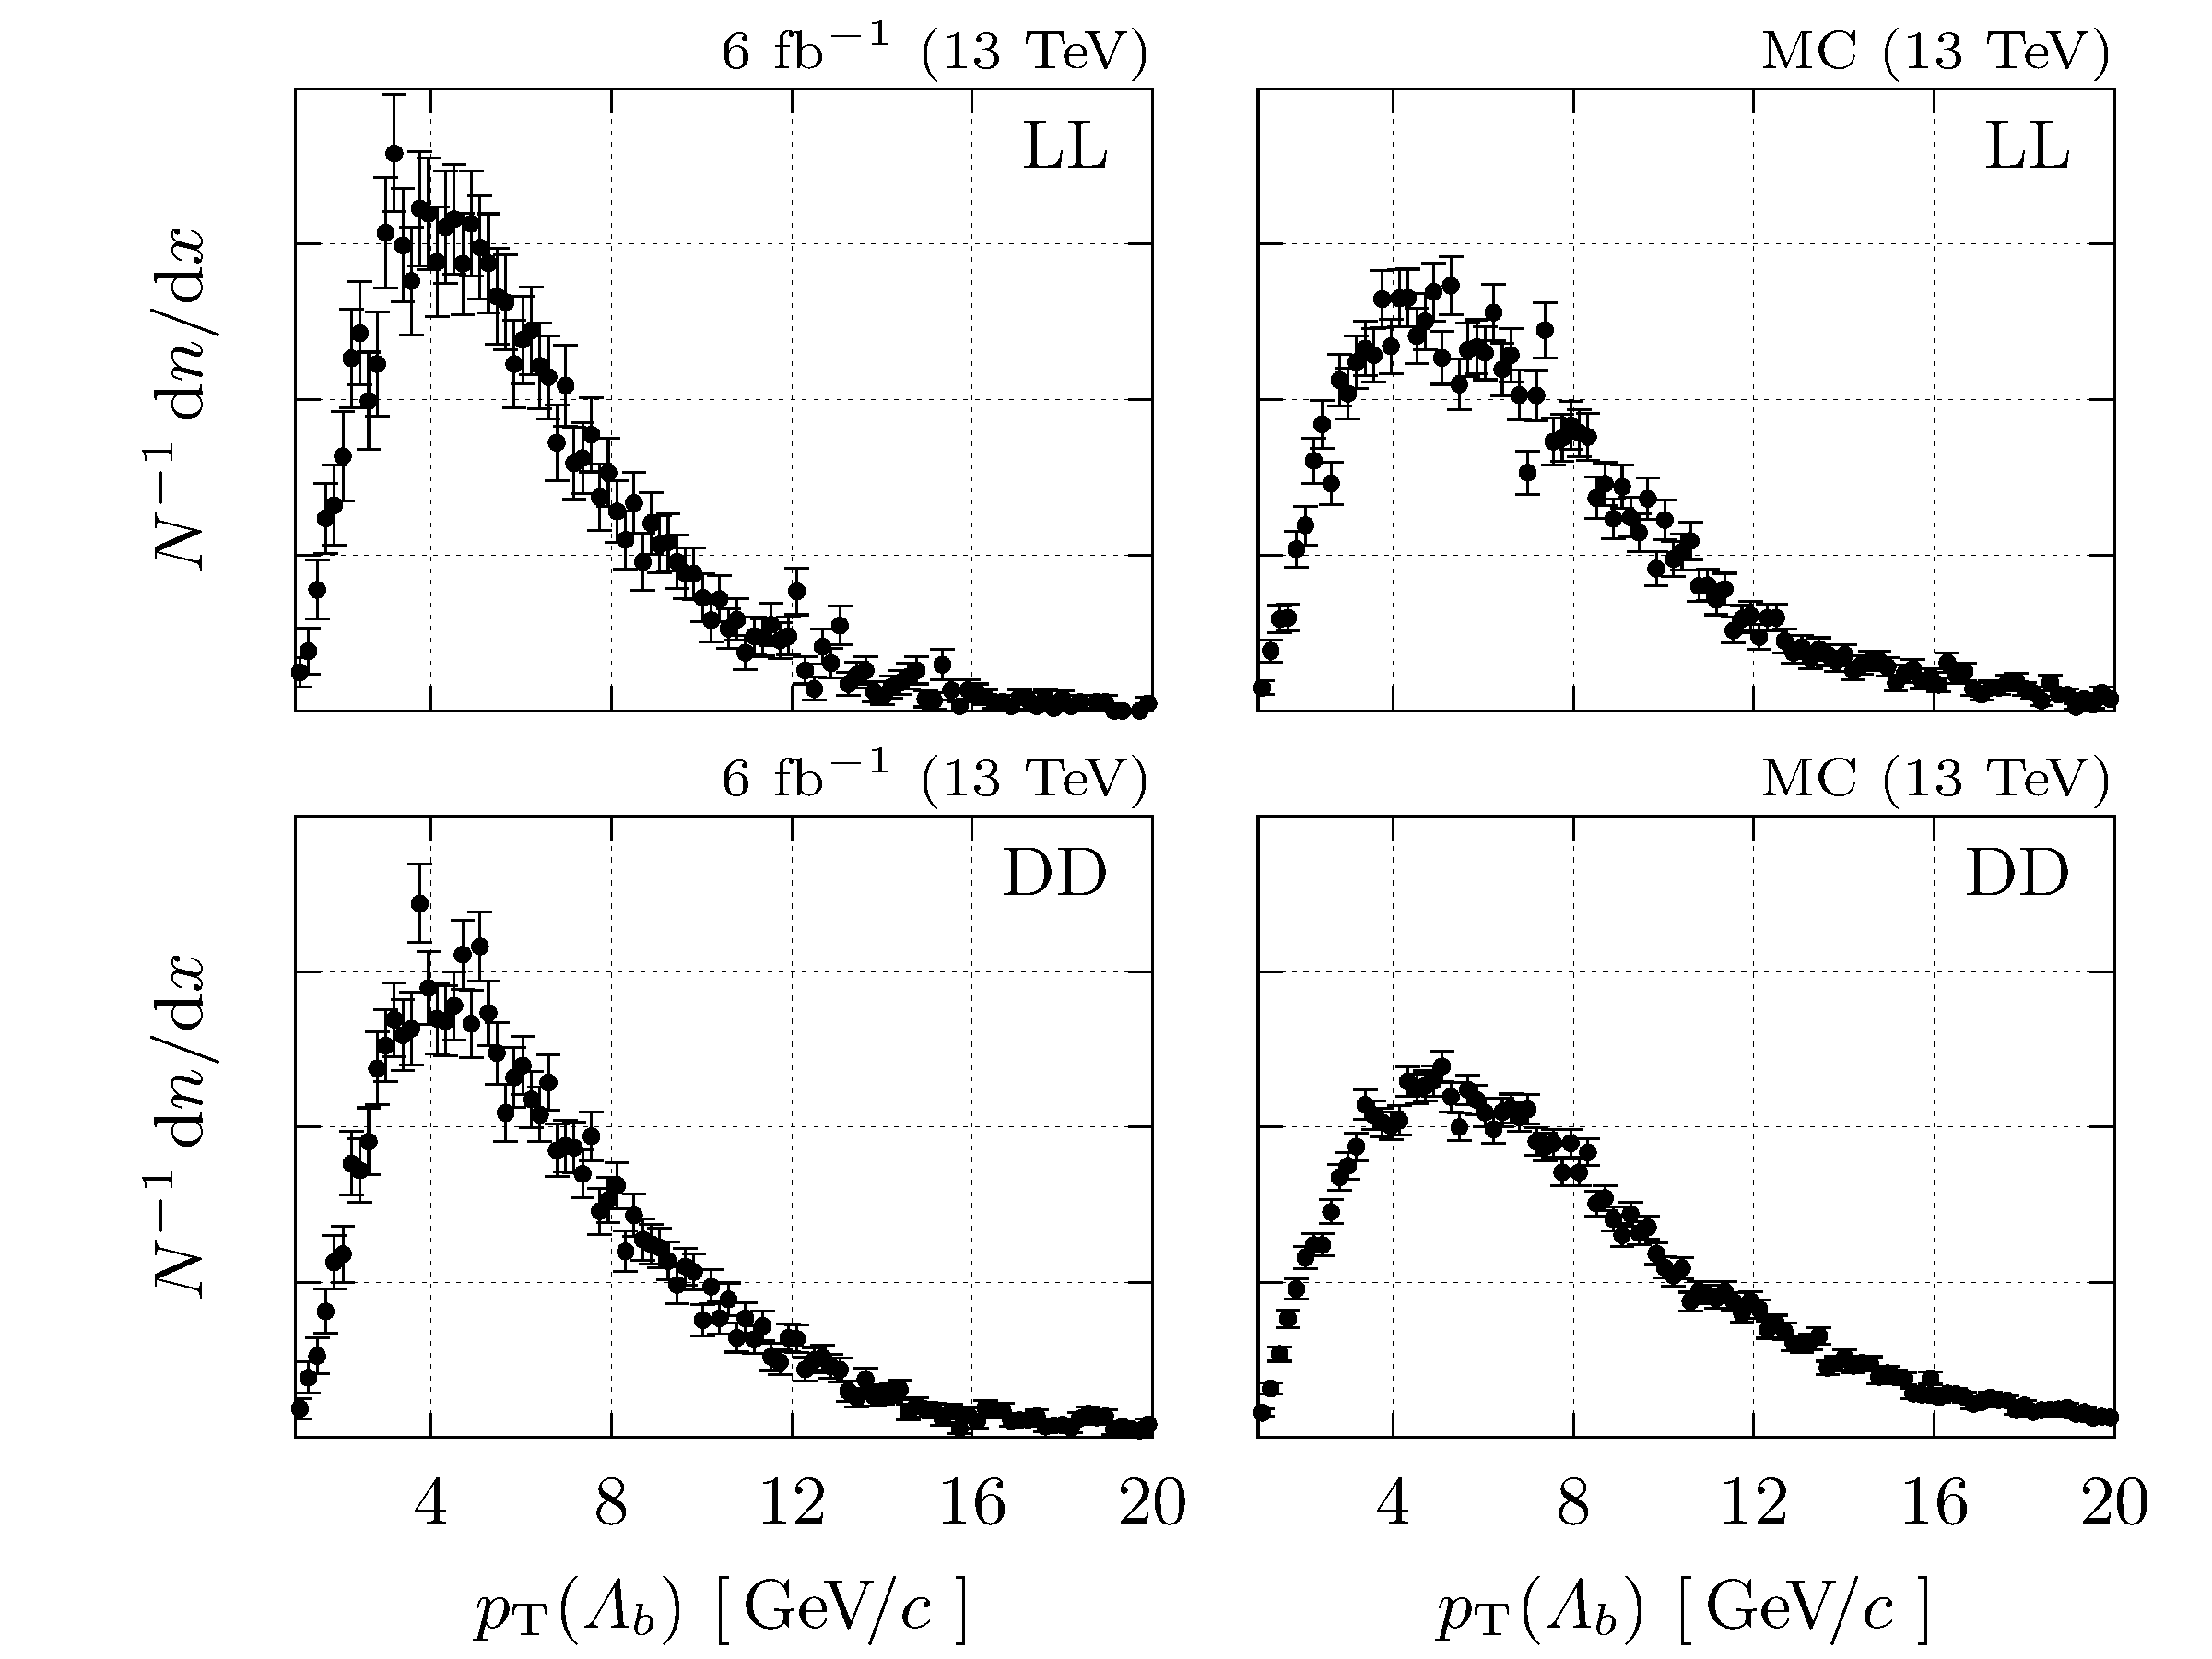
\includegraphics[scale=1.]{Lb2JpsiLz_weighting/hpT_corr.png}
    \caption{Distributions of the transverse momentum of the \Lb baryon for recorded data (left), simulated events (right) and different track types \gls{LL} and \gls{DD} (top and bottom) as obtained from sideband subtractions.}
    \label{fig:LbToJpsiLz_hpT_corr}
\end{figure}

\begin{figure}[htbp]
    \centering
    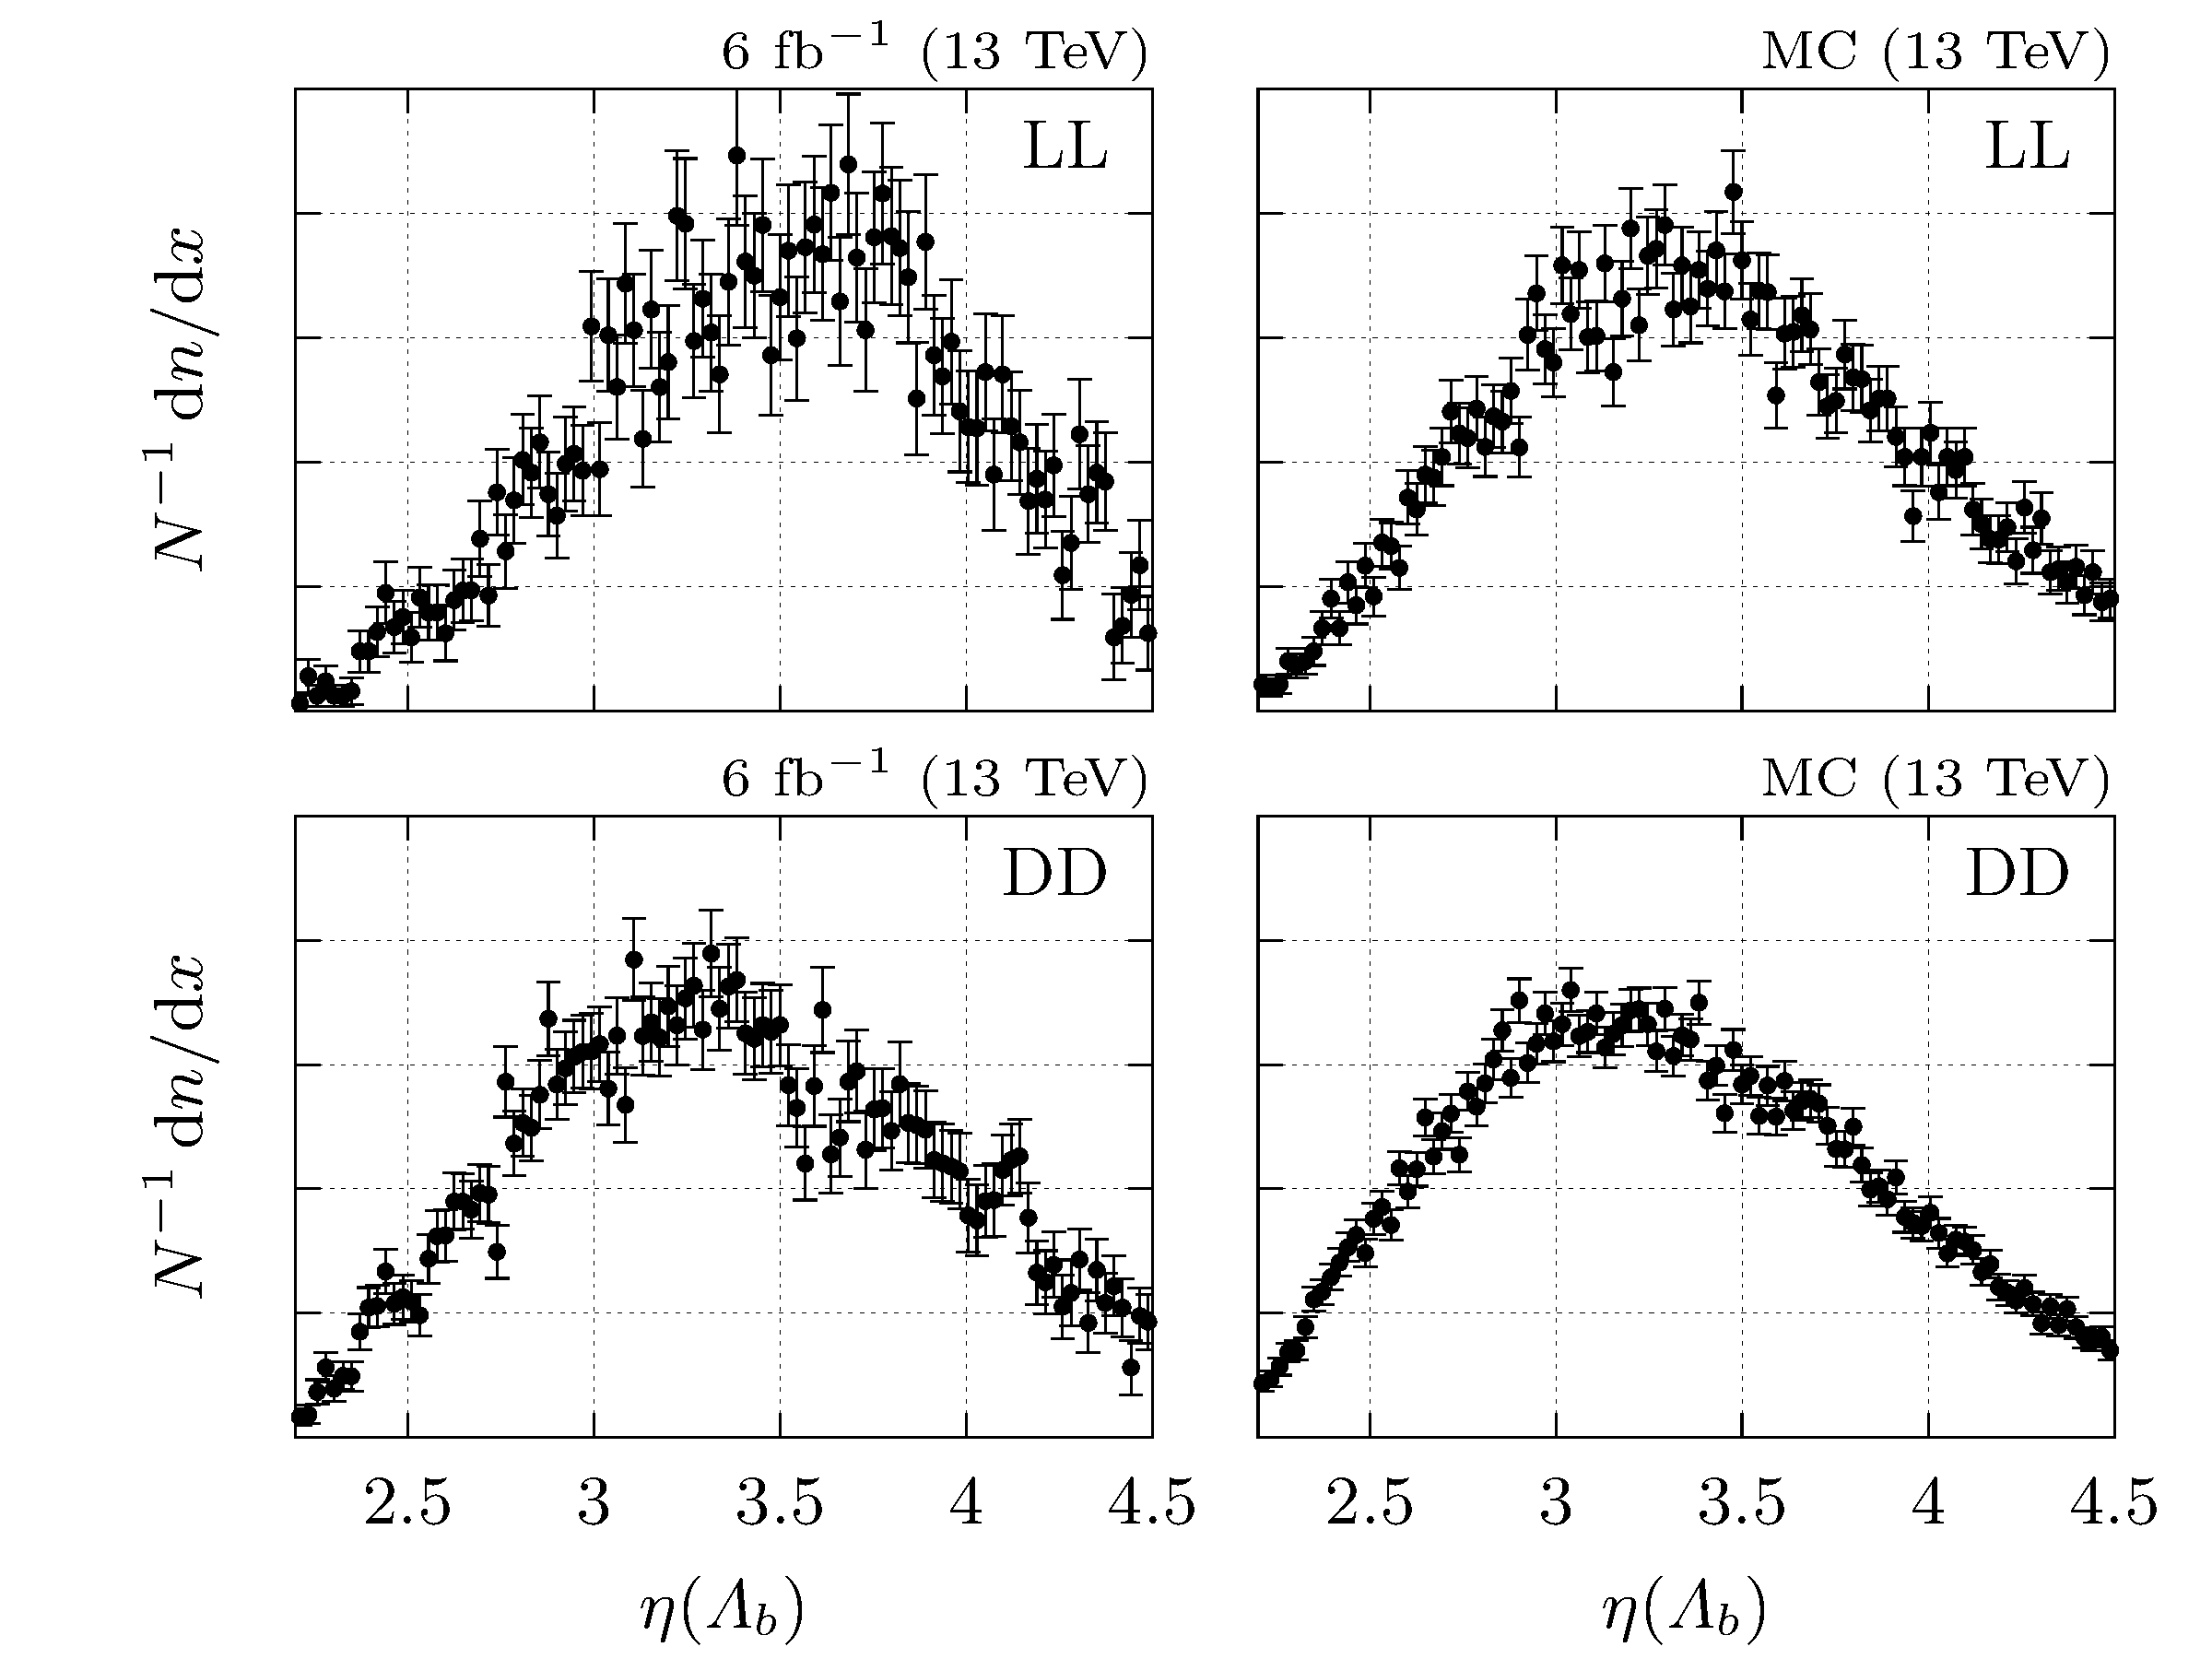
\includegraphics[scale=1.]{Lb2JpsiLz_weighting/heta_corr.png}
    \caption{Distributions of the pseudorapidity of the \Lb baryon for recorded data (left), simulated events (right) and different track types \gls{LL} and \gls{DD} (top and bottom) as obtained from sideband subtractions.}
    \label{fig:LbToJpsiLz_heta_corr}
\end{figure}

\begin{figure}[htbp]
    \centering
    \begin{subfigure}{\textwidth}
        \centering
        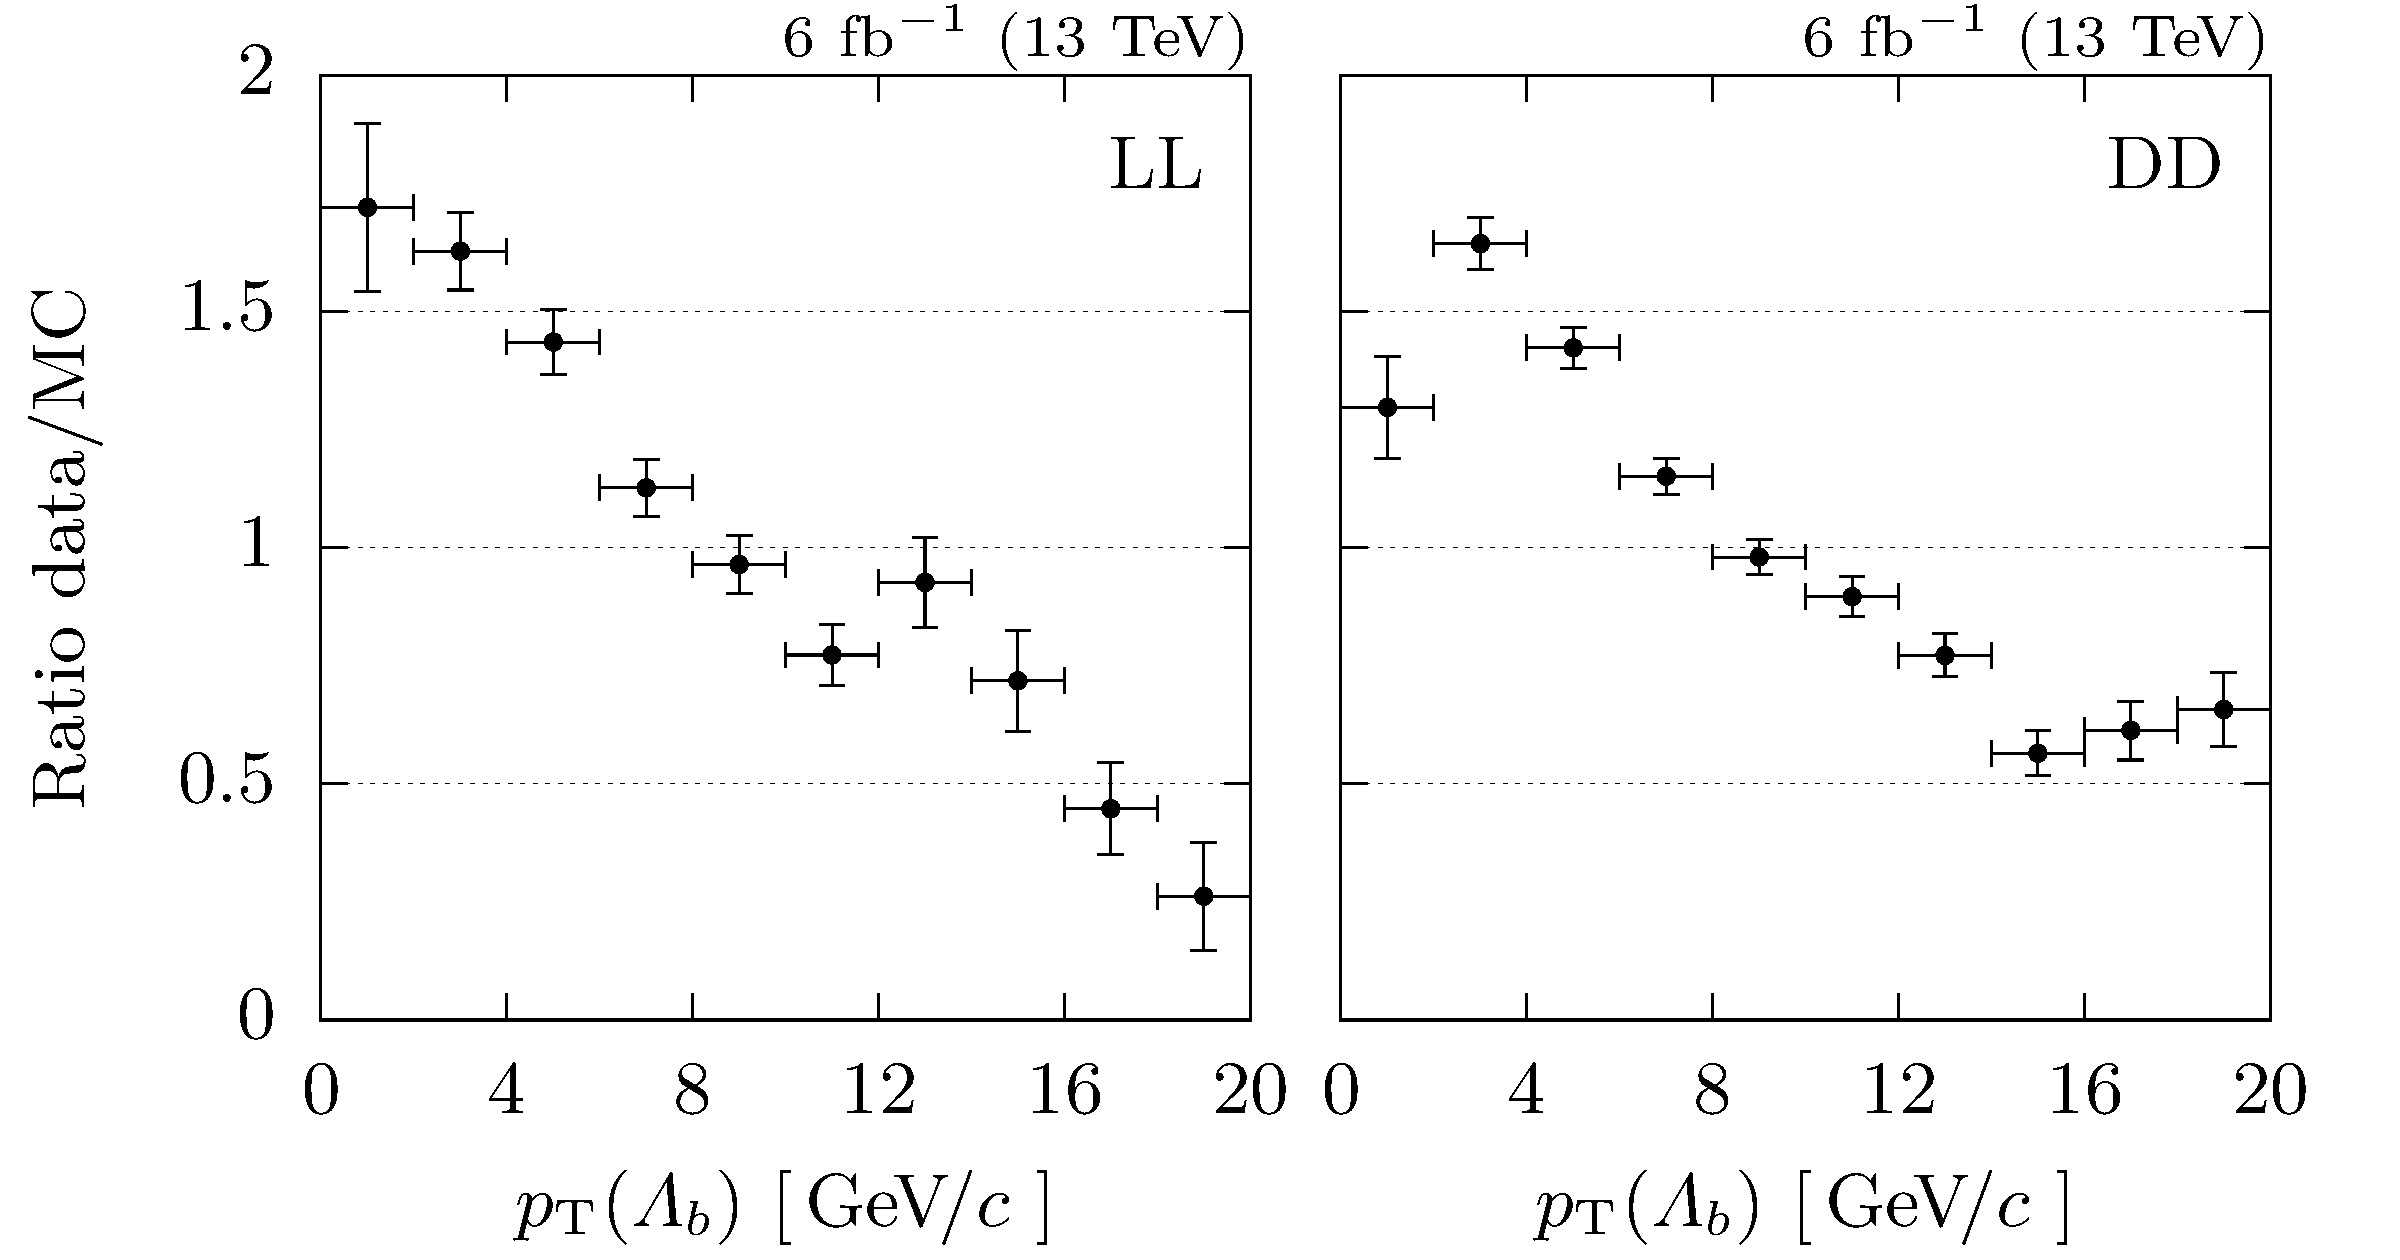
\includegraphics[scale=1.]{Lb2JpsiLz_weighting/hratio_pT.png}
    \end{subfigure}
    \par\bigskip 
    \begin{subfigure}{\textwidth}
        \centering
        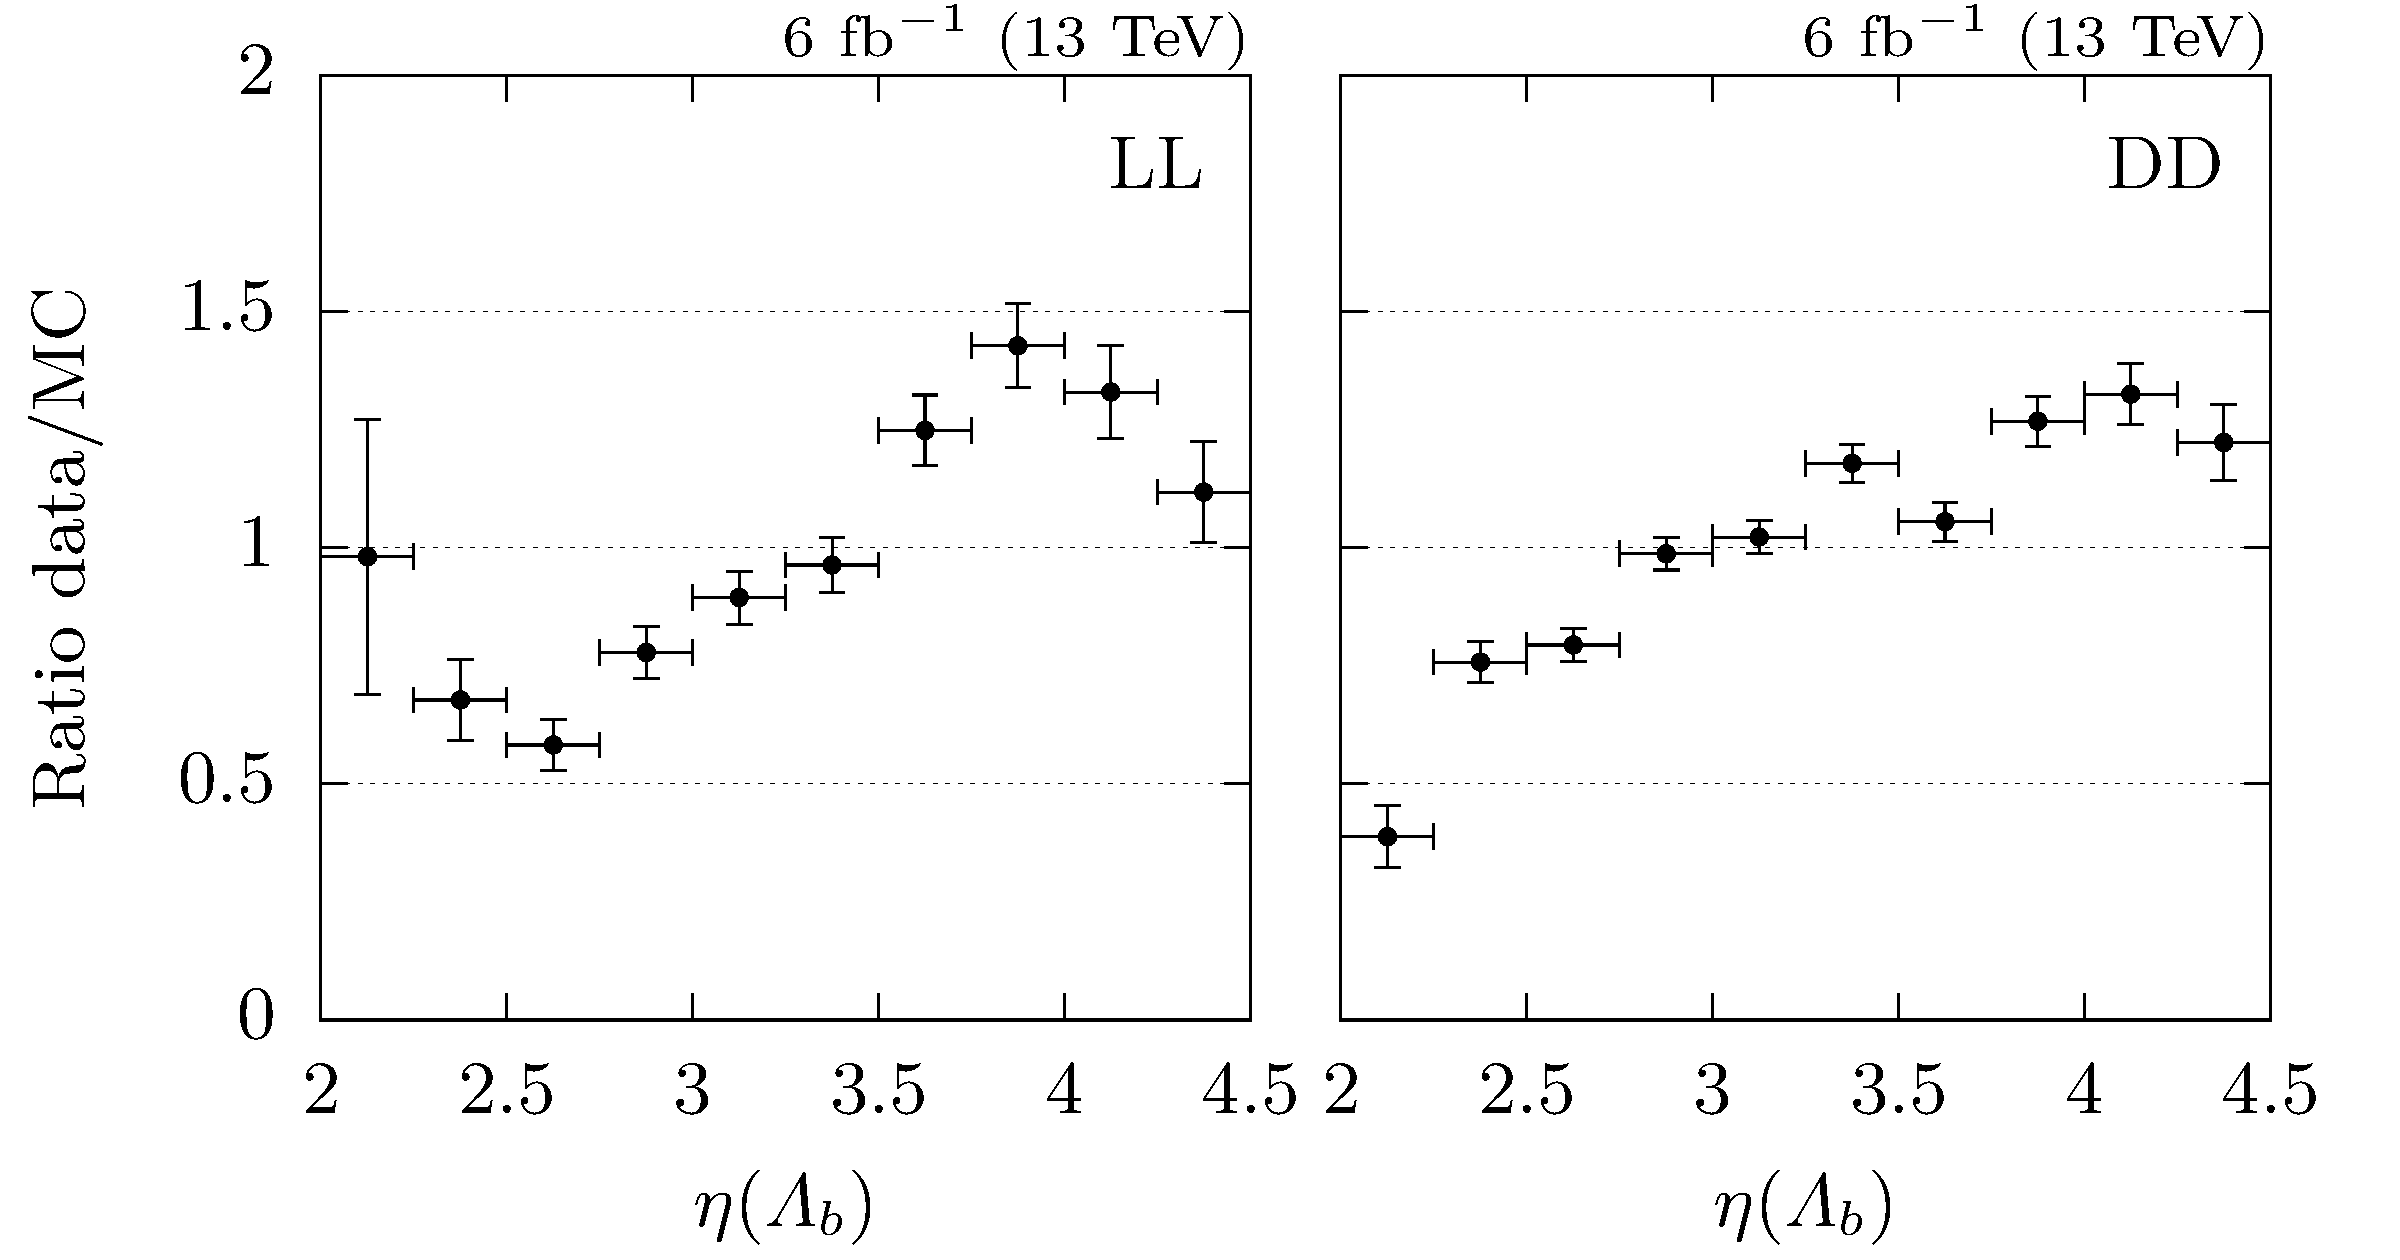
\includegraphics[scale=1.]{Lb2JpsiLz_weighting/hratio_eta.png}
    \end{subfigure}
    \par\bigskip 
    \begin{subfigure}{\textwidth}
        \centering
        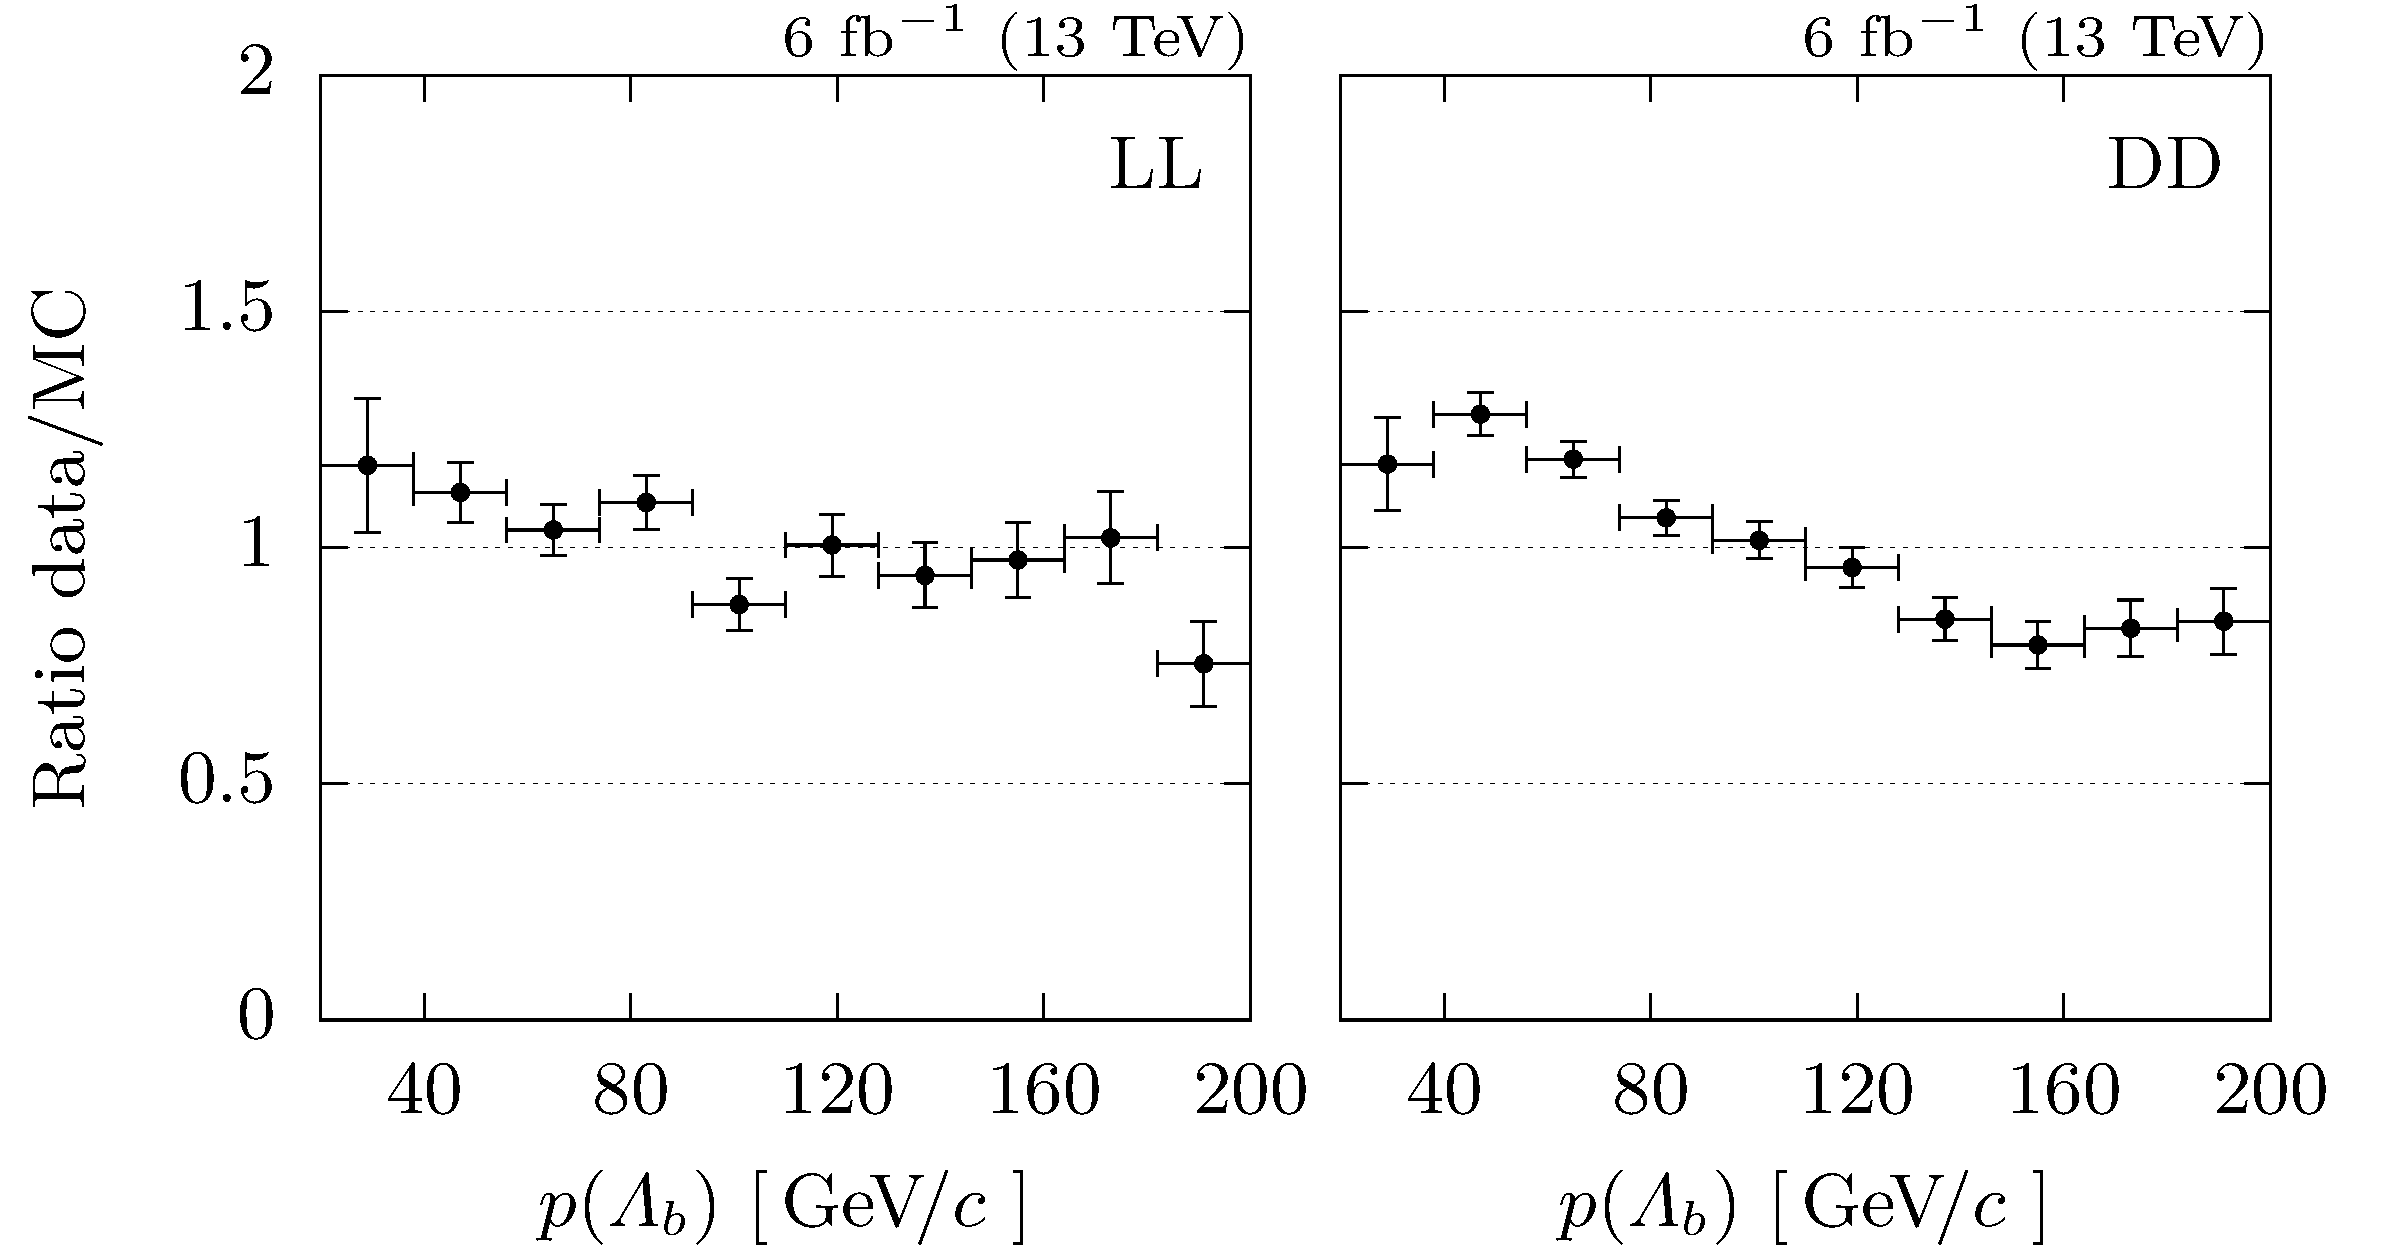
\includegraphics[scale=1.]{Lb2JpsiLz_weighting/hratio_p.png}
    \end{subfigure}
    \par\bigskip 
    \caption{Ratio of the (binned) distributions of the transverse momentum (top), pseudorapidity (middle) and three-momentum magnitude (bottom) of the \Lb baryon for recorded data and \gls{mc} simulated events. The ratios are split w.r.t.\ the track types \gls{LL} (left) and \gls{DD} (right).}
    \label{fig:LbToJpsiLz_hratio}
\end{figure}

After taking the ratios, the histograms are normalized to unity such that in case of a common underlying distribution every bin entry should be one (within uncertainty).
The distributions of the ratios show that this is neither the case for $\pt(\Lb)$ and $\eta(\Lb)$, nor for $p(\Lb)$.
This deviation is expected and motivates the recalibration of the \gls{mc} simulated events with weights.
In the following we will use the distribution of the three-momentum magnitude $p(\Lb)$ to benchmark the performance of the calibration.
If recorded data and simulated events follow the same underlying distribution, the sum
\begin{equation*}
    \chi^2 \equiv \sum_{i=1}^n \chi_i^2
\end{equation*}
of the normalized deviation from one $\chi_i^2$ for each bin $i$,
\begin{equation*}
    \chi_i^2 \equiv \left( \frac{r_i - 1}{u(r_i)} \right)^2 \,,
\end{equation*}
where $r_i$ and $u(r_i)$ is the central value and its uncertainty of the $i$-th bin, respectively, is then $\chi^2$-distributed with $n$ \gls{dof} (number of bins).
For \gls{LL} (\gls{DD}) we find $\chi^2 \approx 21$ ($\chi^2 \approx 109$) and thus reject the hypothesis of a common underlying distribution for recorded data and simulated events on a $>98\,\%$ confidence level according to Eq.~\eqref{eq:fitprob}.

Weights are calculated by taking the binned, normalized ratio of the marginal distributions of recorded and simulated events for \pt or $\eta$ in subsequent steps.
The data set is split w.r.t.\ the track types \gls{LL} and \gls{DD}.
The resulting histograms of ratios $w_1(\pt)$ and $w_2(\eta)$, binned for the given quantity \pt and $\eta$, are then used to calculated the \pt and $\eta$ dependent weight $w(\pt, \eta) := w_1(\pt) \times w_2(\eta)$ for a given simulated event.
The iteration procedure is structured as following:
\begin{enumerate}[itemsep=2pt,parsep=2pt]
    \item Initialize all weights with one.
    \item Update $w_1(\pt)$ using weight factors from the previous iteration.
    \item Update $w(\pt, \eta) = w_1(\pt) \times w_2(\eta)$.
    \item Update $w_2(\eta)$ using the updated $w_1(\pt)$ and $w_2(\eta)$ from the previous iteration.
    \item Update $w(\pt, \eta) = w_1(\pt) \times w_2(\eta)$.
    \item Continue with step 2 until convergence is reached. 
\end{enumerate}
%By design, at the end of each iteration, the ratio of recorded data and weighted simulated events should be one in the marginal distribution of $\eta(\Lb)$.
Each iteration yields a factor $w_1(\pt)$ and $w_2(\eta)$ for a given \pt and $\eta$ bin.
The final weights are their product.
%, \ie{}, $$w(\pt, \eta) = w_1(\pt) \times w_2(\eta).$$
The convergence of this approach is measured in the weight update for each bin, separately.

Starting from the first iteration the histograms for (weighted) simulated events are filled with tuples of the particle event with an associated weight $(x_i, w_i)$.
After filling, the content of a bin~$j$ is the sum of its weights~$w^{(j)}_i$ and the associated uncertainty~$u^{(j)}$ is
\begin{equation*}
    u^{(j)} = \sqrt{ \sum_i \left( w^{(j)}_i \right)^2 } \,.
\end{equation*}
We note that for $w^{(j)}_i = 1~\forall i,j$ this scheme is equivalent to unweighted events where the uncertainty of each bin with bin content $n$ is given by $\sqrt n$.

\begin{figure}[htbp]
    \centering
    \begin{subfigure}{\textwidth}
        \centering
        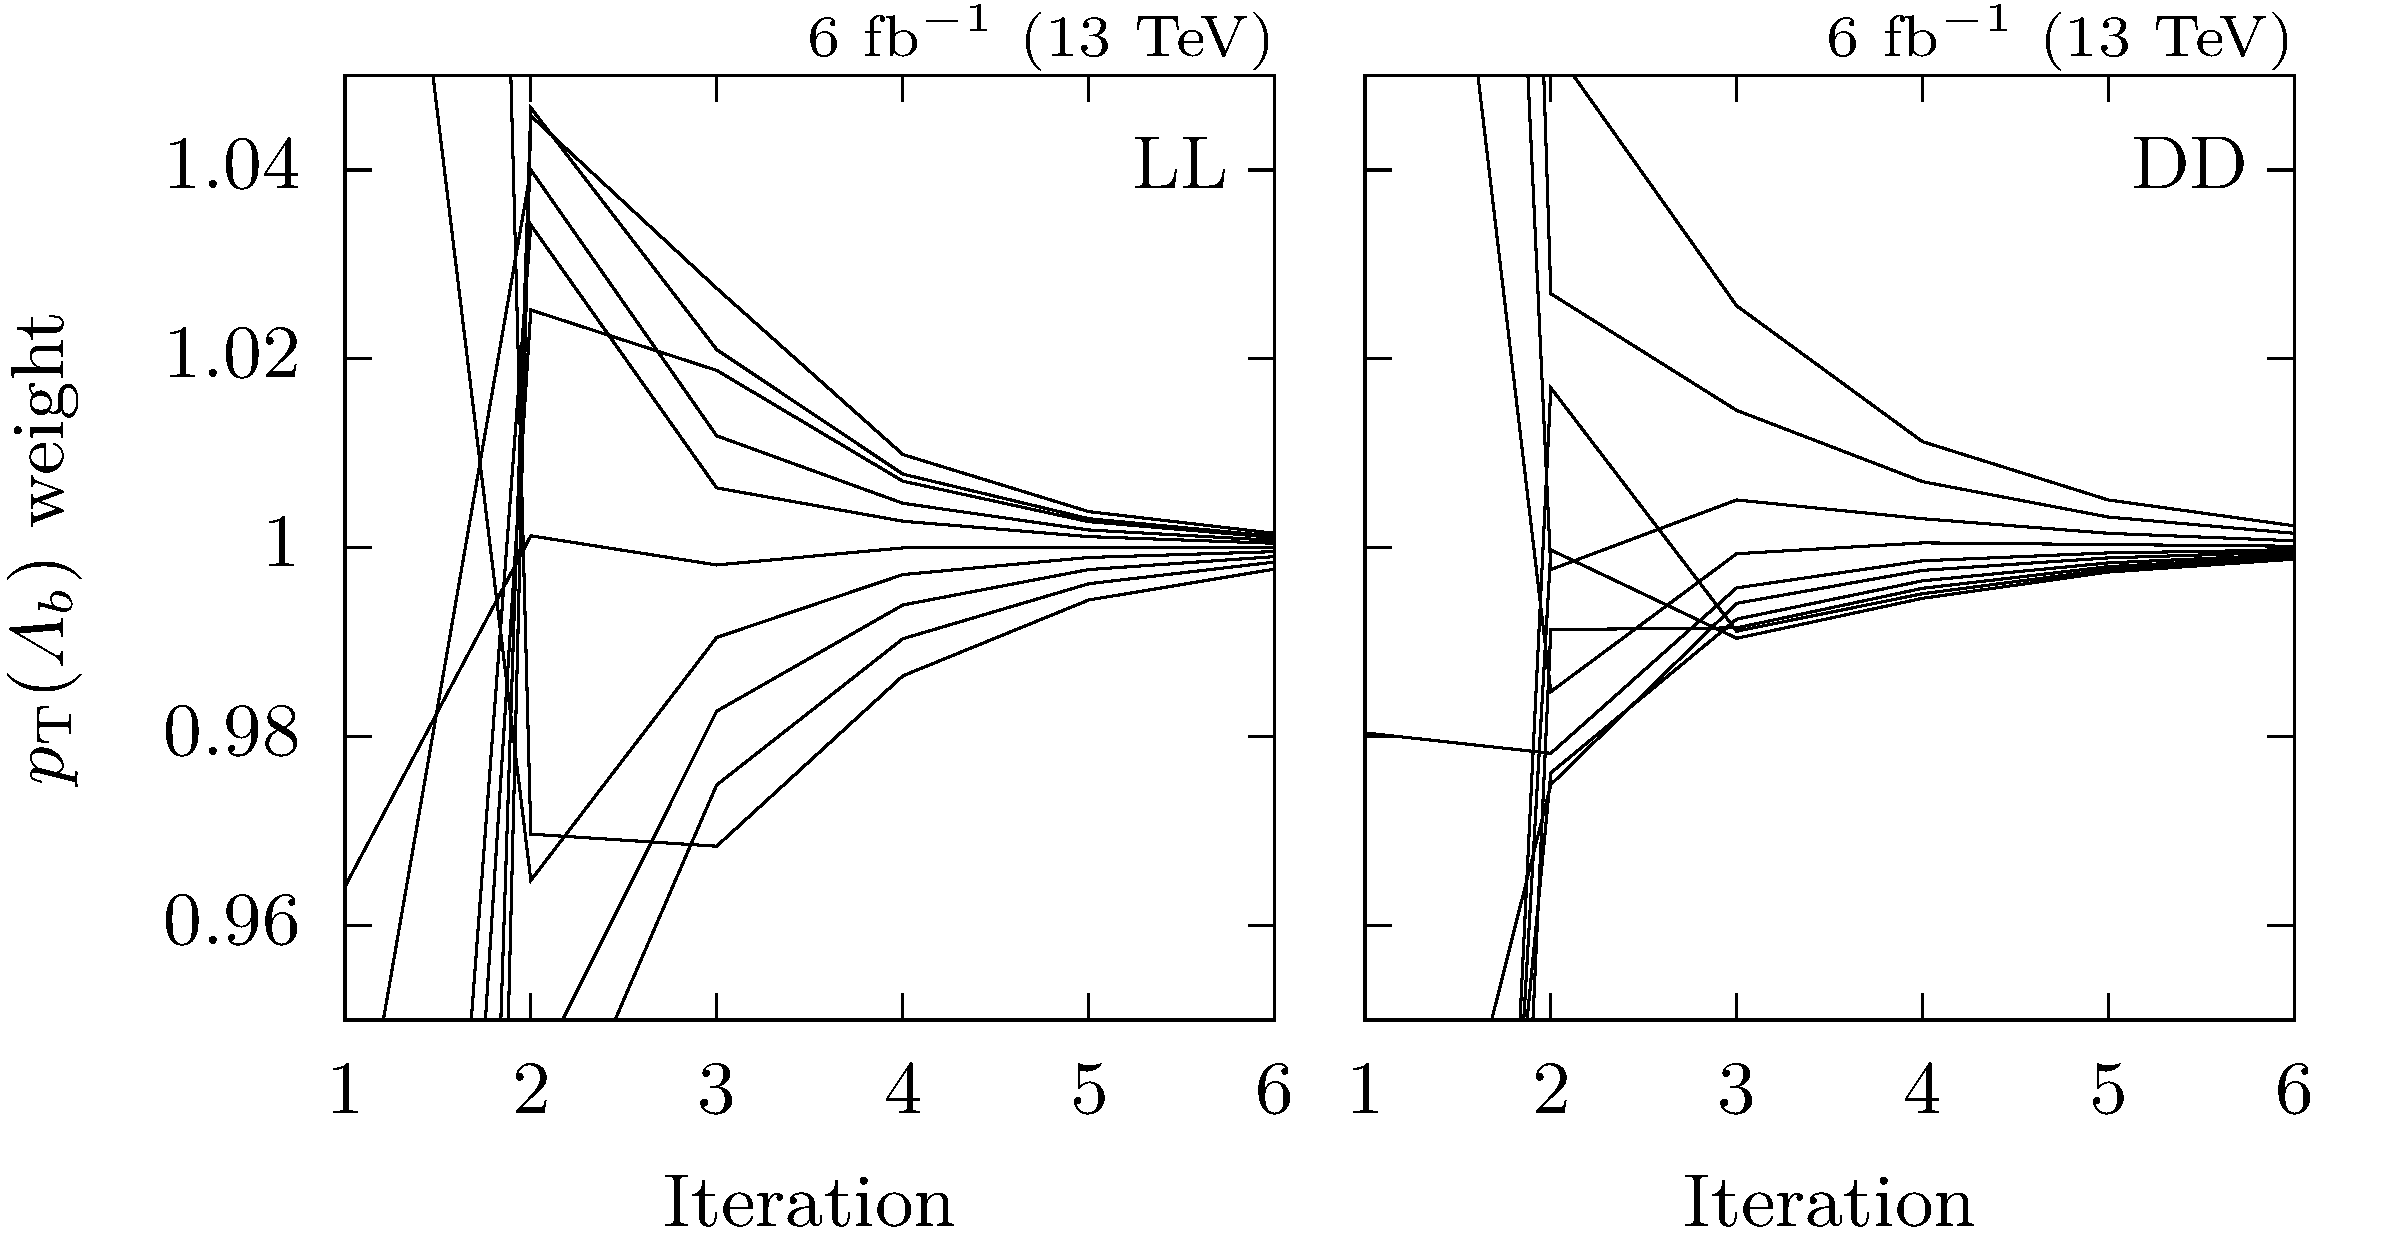
\includegraphics[scale=1.]{Lb2JpsiLz_weighting/conv_pT.png}
    \end{subfigure}
    \par\bigskip 
    \begin{subfigure}{\textwidth}
        \centering
        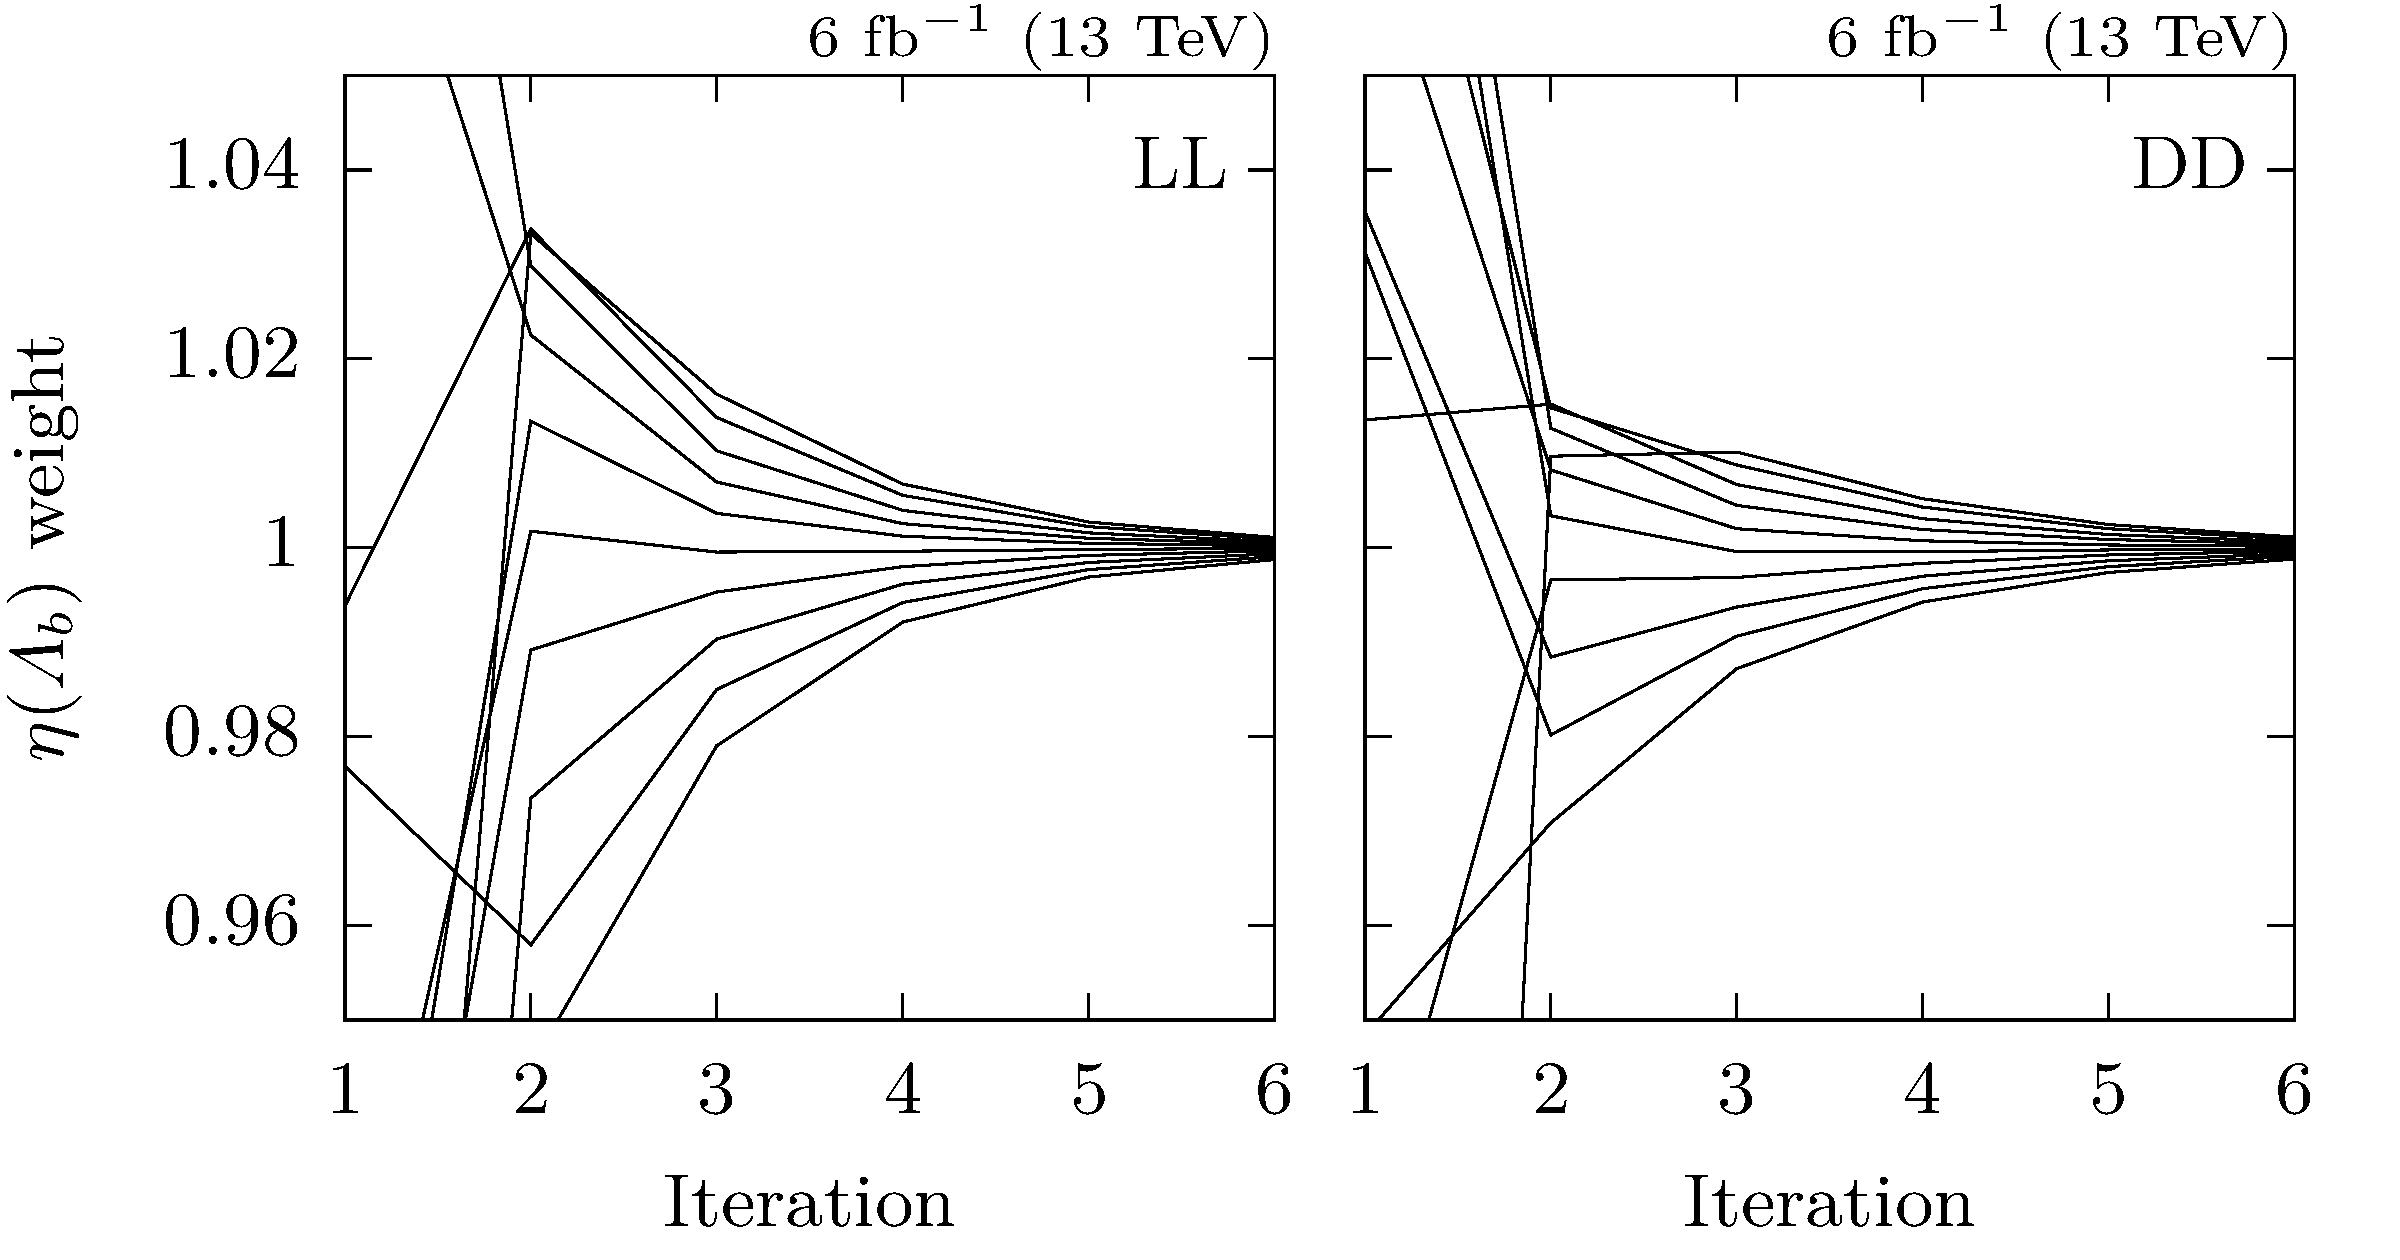
\includegraphics[scale=1.]{Lb2JpsiLz_weighting/conv_eta.png}
    \end{subfigure}
    \caption{Convergence of $w_1(\pt)$ (top) and $w_2(\eta)$ (bottom) during the iterative weighting process for \gls{LL} and \gls{DD} tracks (left and right).}
    \label{fig:LbToJpsiLz_conv}
\end{figure}

In Fig.~\ref{fig:LbToJpsiLz_conv} we show the convergence of the iterative weighting process for \gls{LL} and \gls{DD} tracks.
Each solid line is the weight update of a bin as a function of the iteration number.
Convergence is achieved when all multiplicative updates have approached the value one.
In the above case, we stop the iteration after six iterations and consider the product of all weight updates (starting with the value one of the zeroth iteration) as the converged final weight for each bin.

The significance of the obtained weights is quantized in the $p$-values corresponding to the hypothesis of a common underlying distribution for recorded and simulated events, \ie{}, $w_1(p_T)=1$ and $w_2(\eta)=1$, respectively.
These $p$-values are listed in Tab.~\ref{tab:LbToJpsiLz_pvalues} after six successive iterations.
Incompatibilities with these hypotheses are expected and indicate the necessity of the scaling process, whereas the $p$-value for $r(p)=1$, where $r(p)$ is the (binned) ratio of the three-momentum magnitude distribution of recorded data and simulated events, exhibits the improvement of features that are scaled implicitly due to correlations with \pt and $\eta$.
The change of $r(p)$ during the iterations is also listed in Tab.~\ref{tab:LbToJpsiLz_pvalues} and shows the improvement of the fidelity of the \gls{mc} simulated events due to the scaling with $w(\pt,\eta)$.

%\begin{figure}[htbp]
%    \centering
%    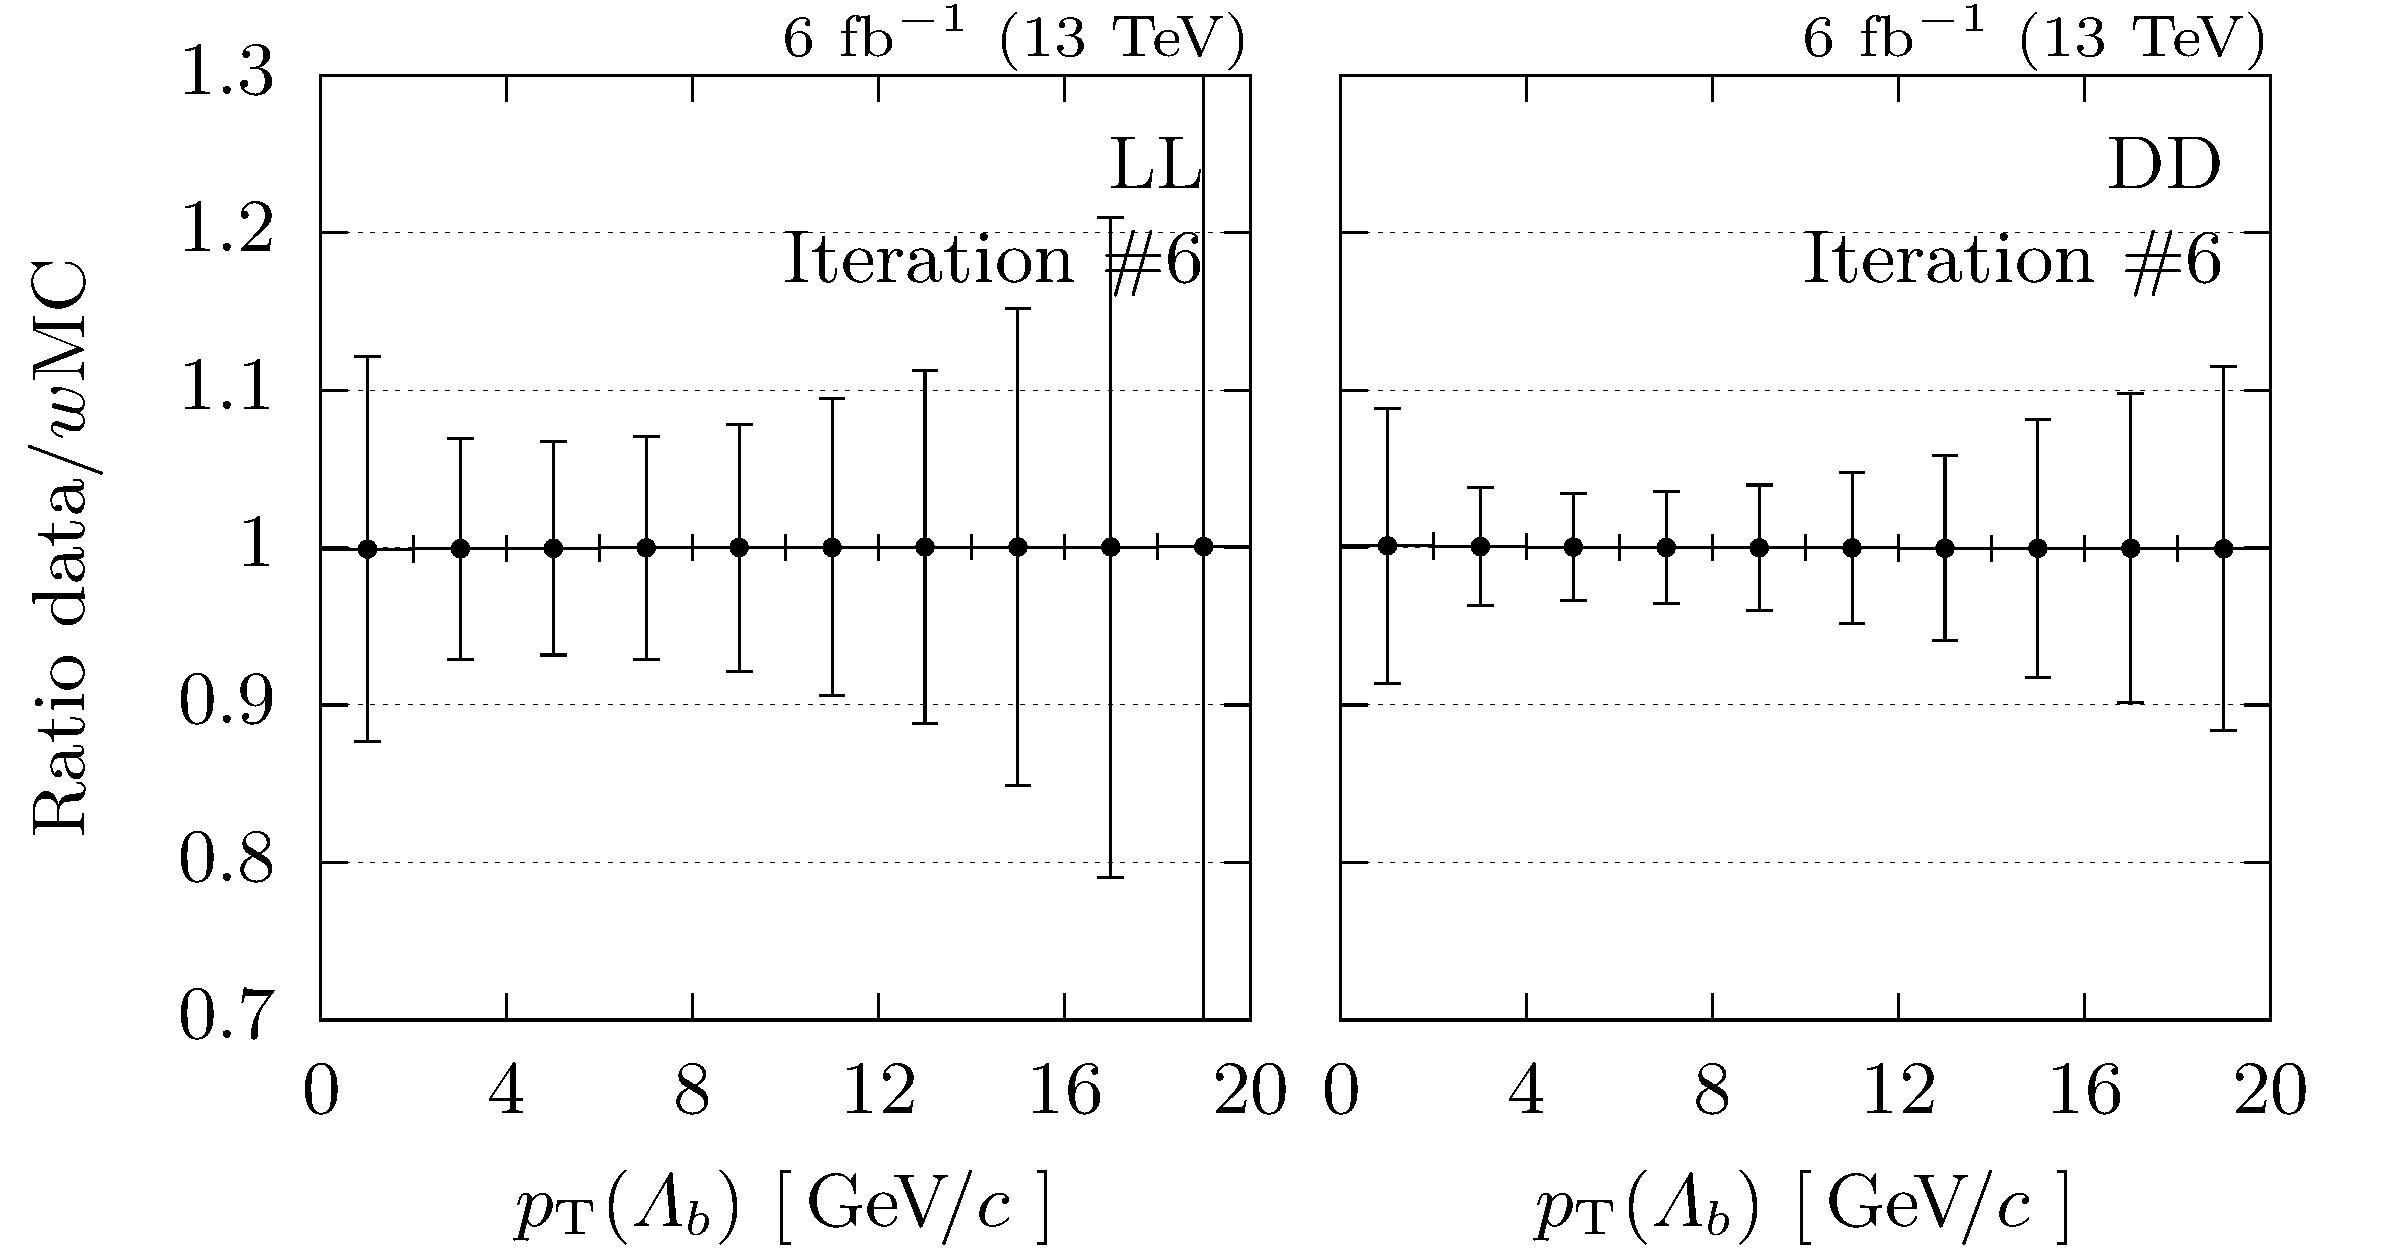
\includegraphics[scale=1.]{Lb2JpsiLz_weighting/hratio_pT_final.png}
%    \caption{Ratio of recorded data and weighted MC simulated events after six successive iterations in $\pt(\Lb)$ bins.}
%\end{figure}

%\begin{figure}[htbp]
%    \centering
%    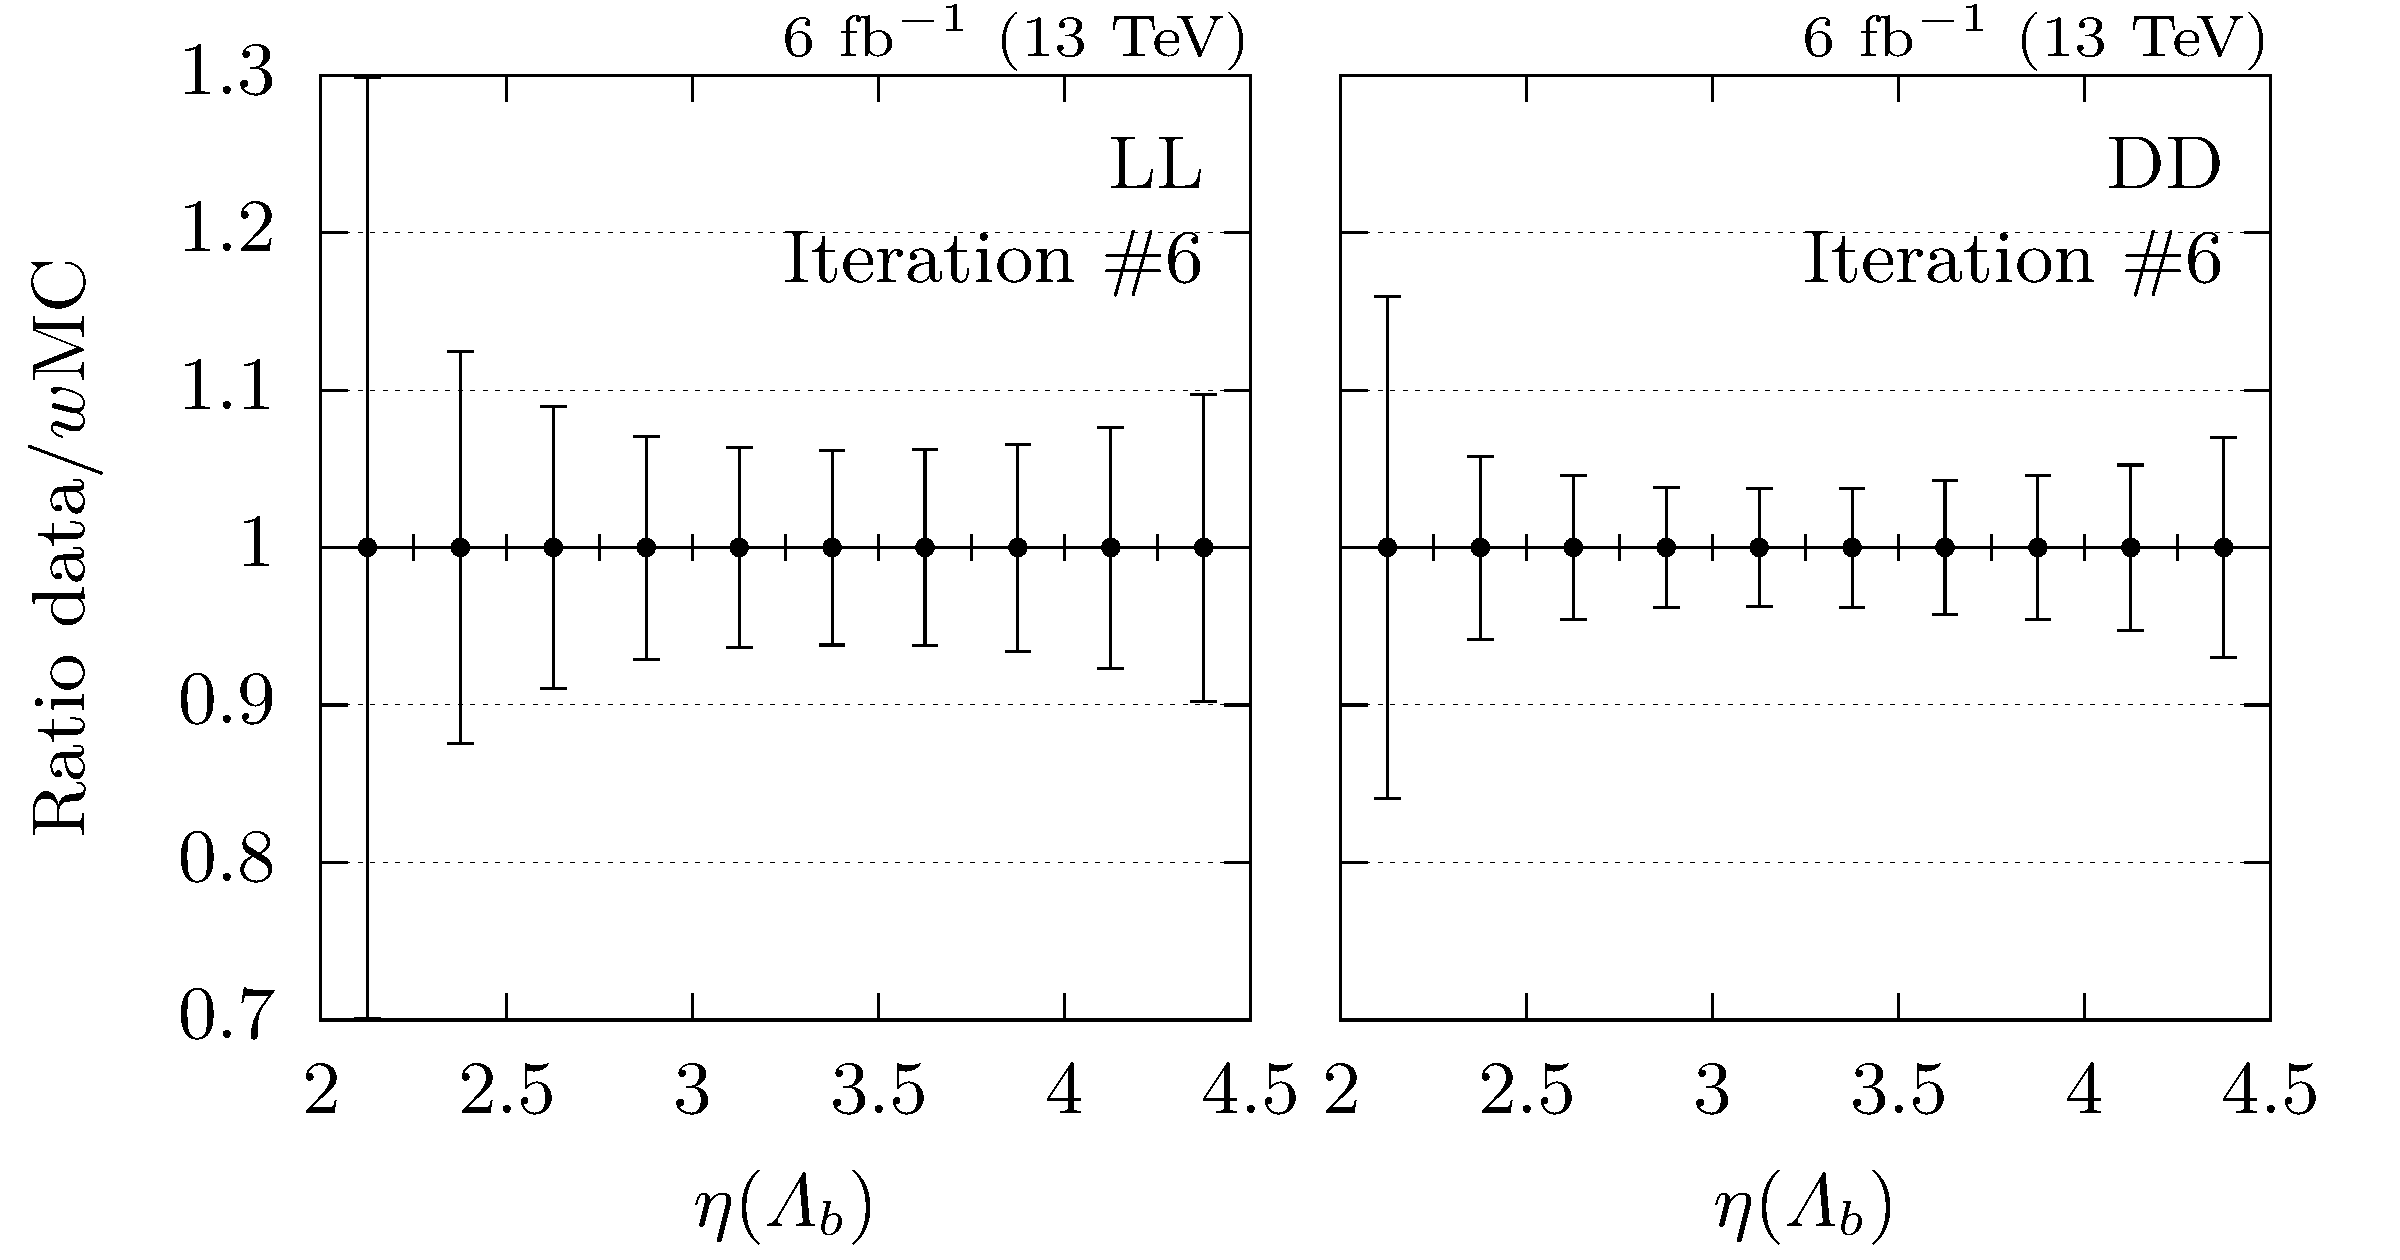
\includegraphics[scale=1.]{Lb2JpsiLz_weighting/hratio_eta_final.png}
%    \caption{Ratio of recorded data and weighted MC simulated events after six successive iterations in $\eta(\Lb)$ bins.}
%\end{figure}

%\begin{figure}[htbp]
%    \centering
%    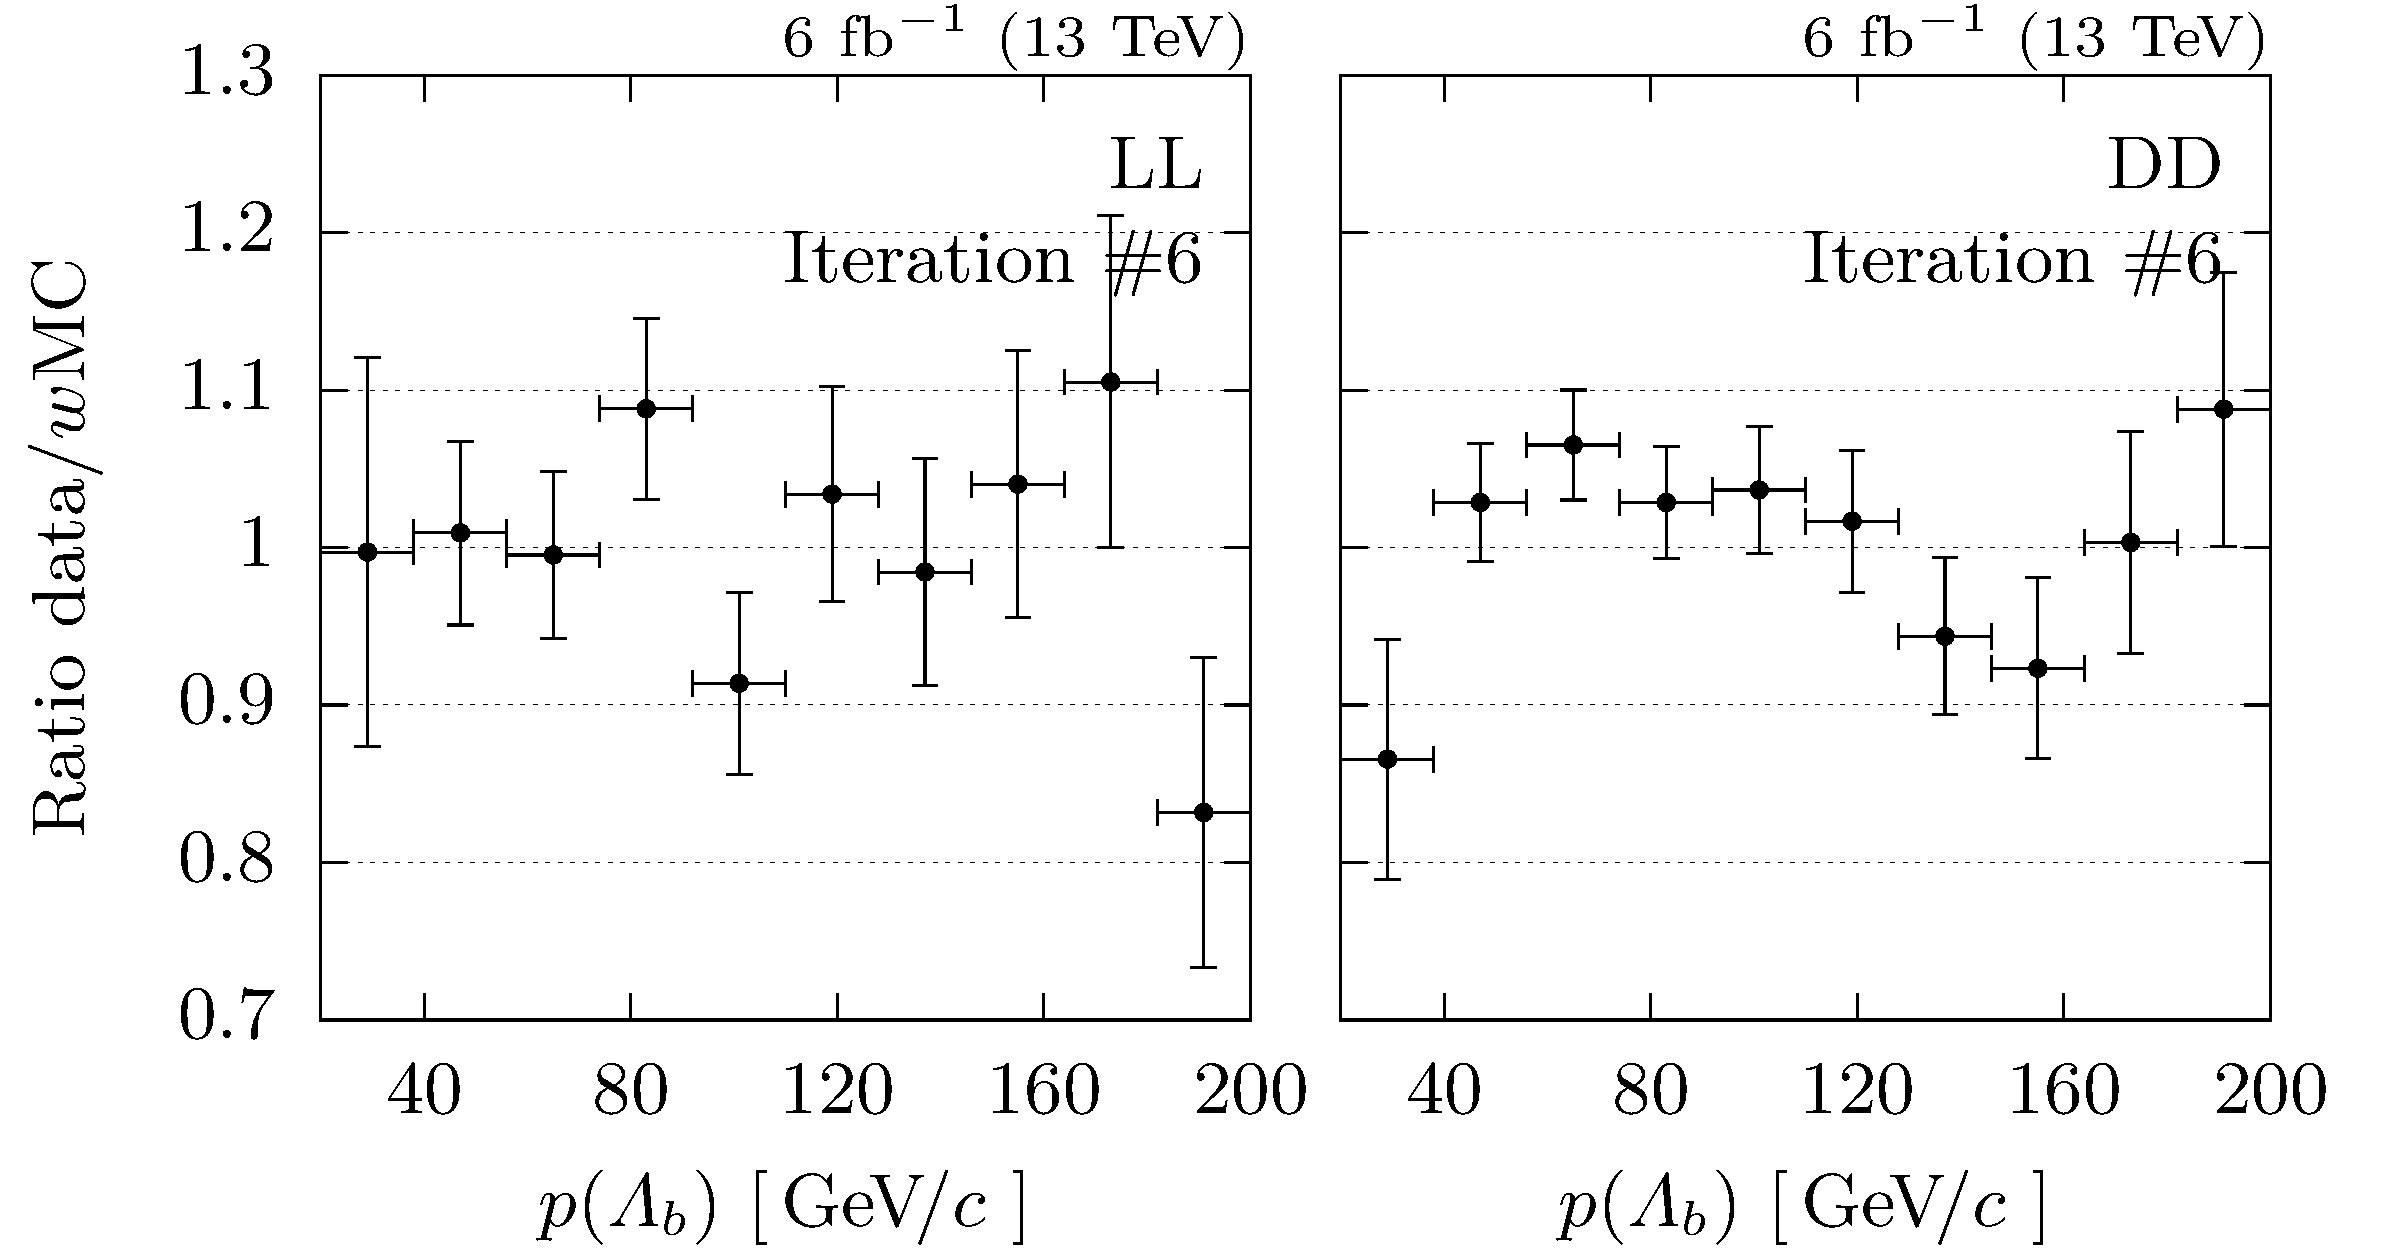
\includegraphics[scale=1.]{Lb2JpsiLz_weighting/hratio_p_final.png}
%    \caption{Ratio of recorded data and weighted MC simulated events after six successive iterations in $p(\Lb)$ bins.}
%\end{figure}

\begin{figure}[htbp]
    \centering
    \begin{subfigure}{\textwidth}
        \centering
        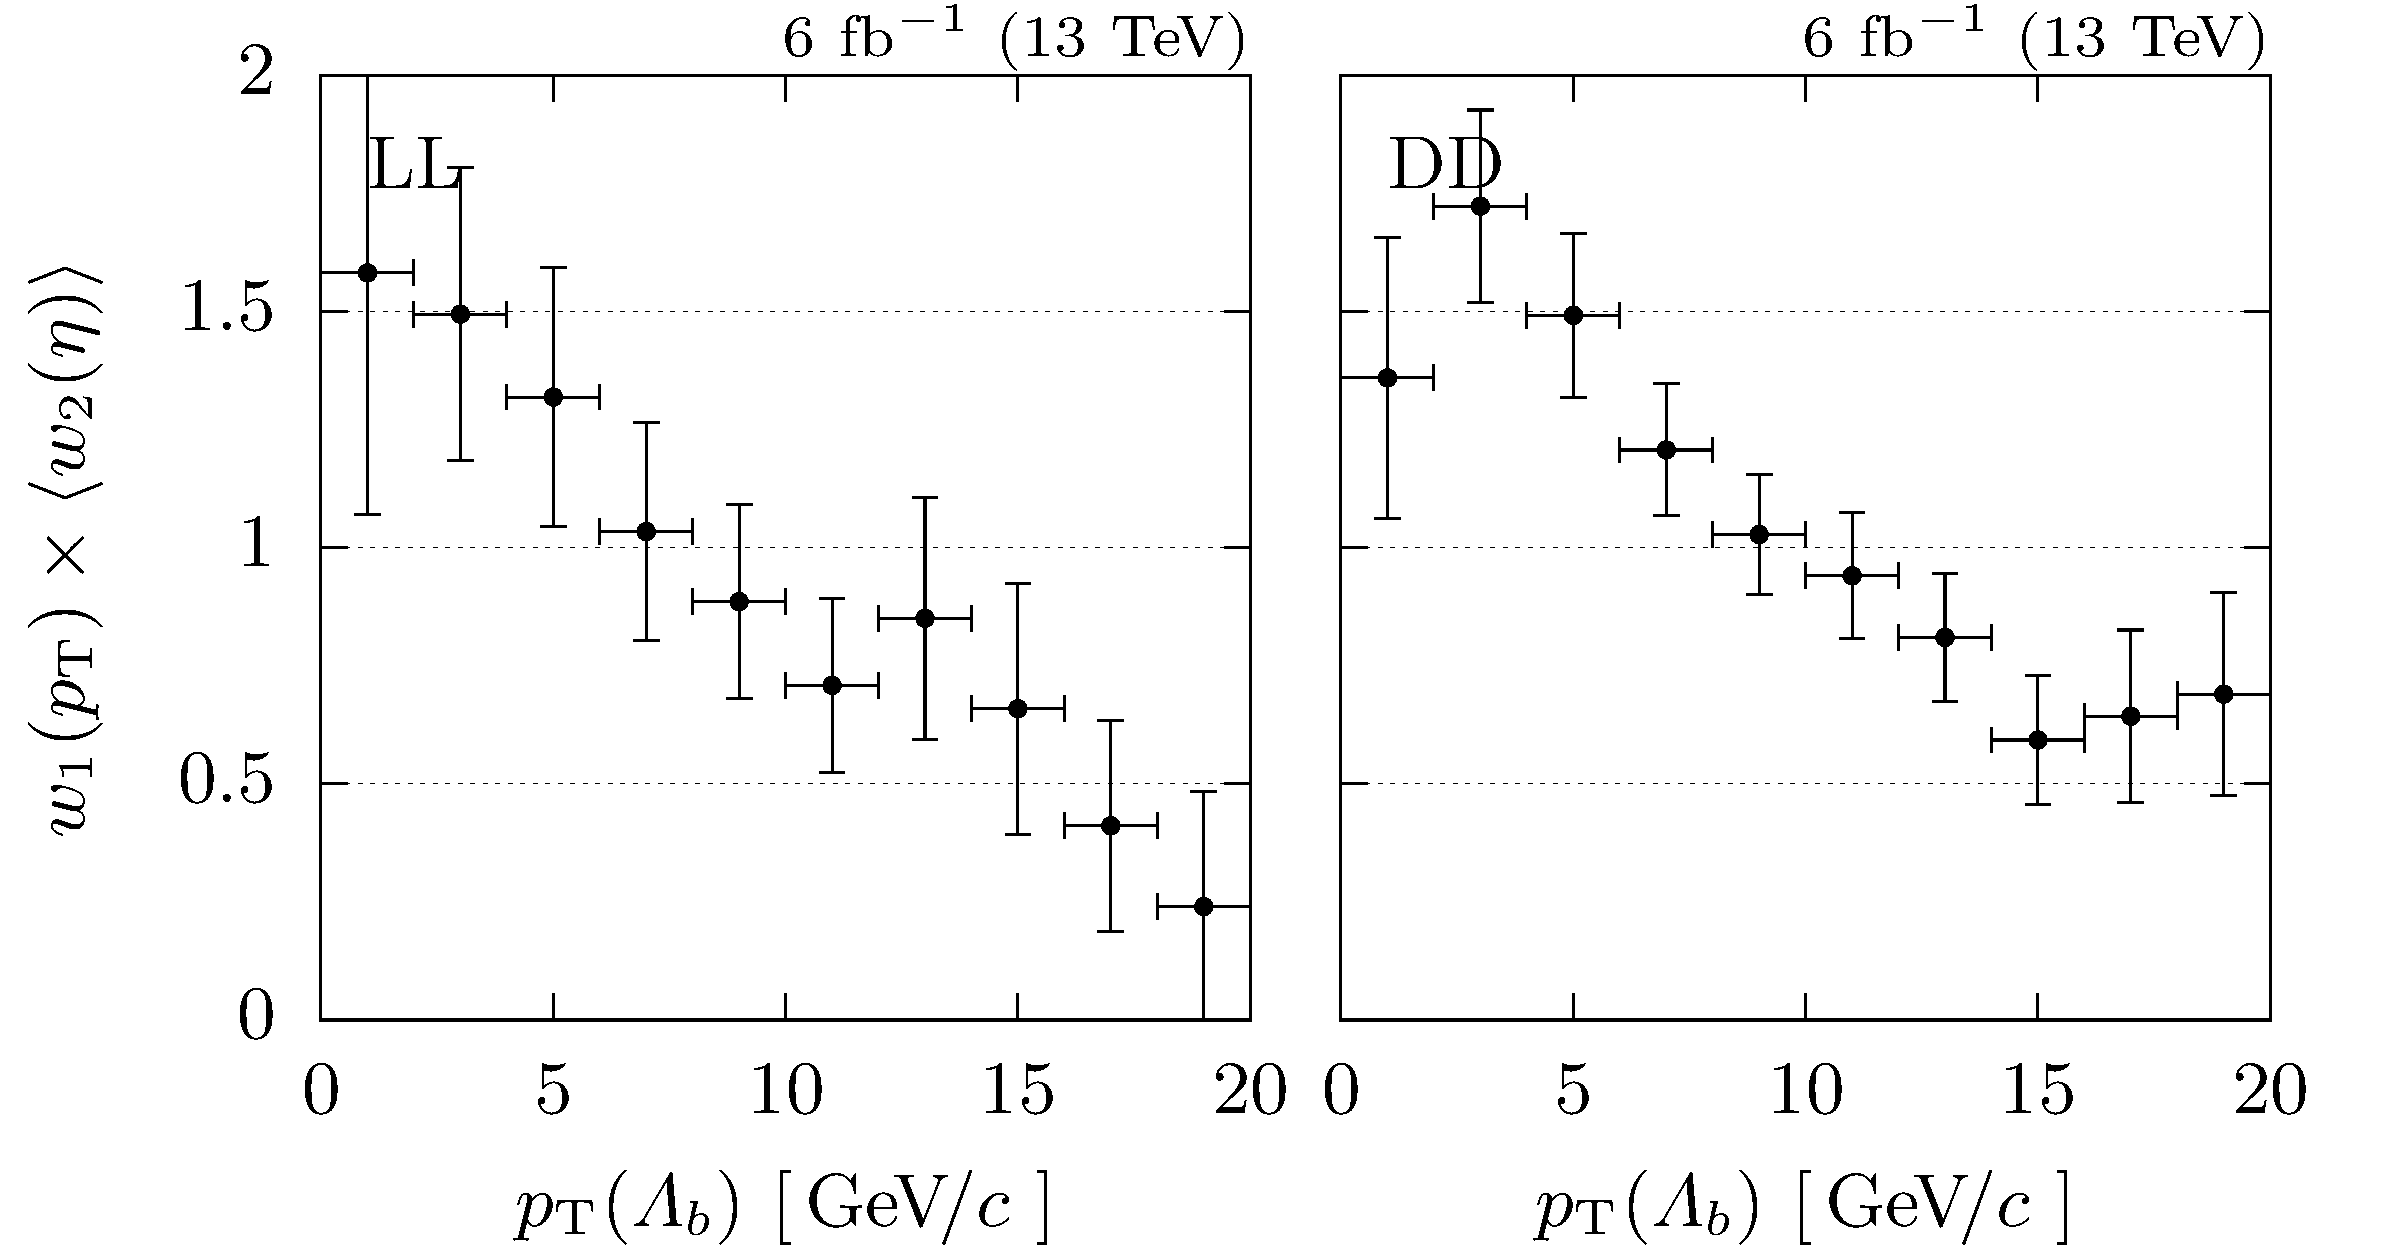
\includegraphics[scale=1.]{Lb2JpsiLz_weighting/avgw_prod_pT.png}
    \end{subfigure}
    \par\bigskip 
    \begin{subfigure}{\textwidth}
        \centering
        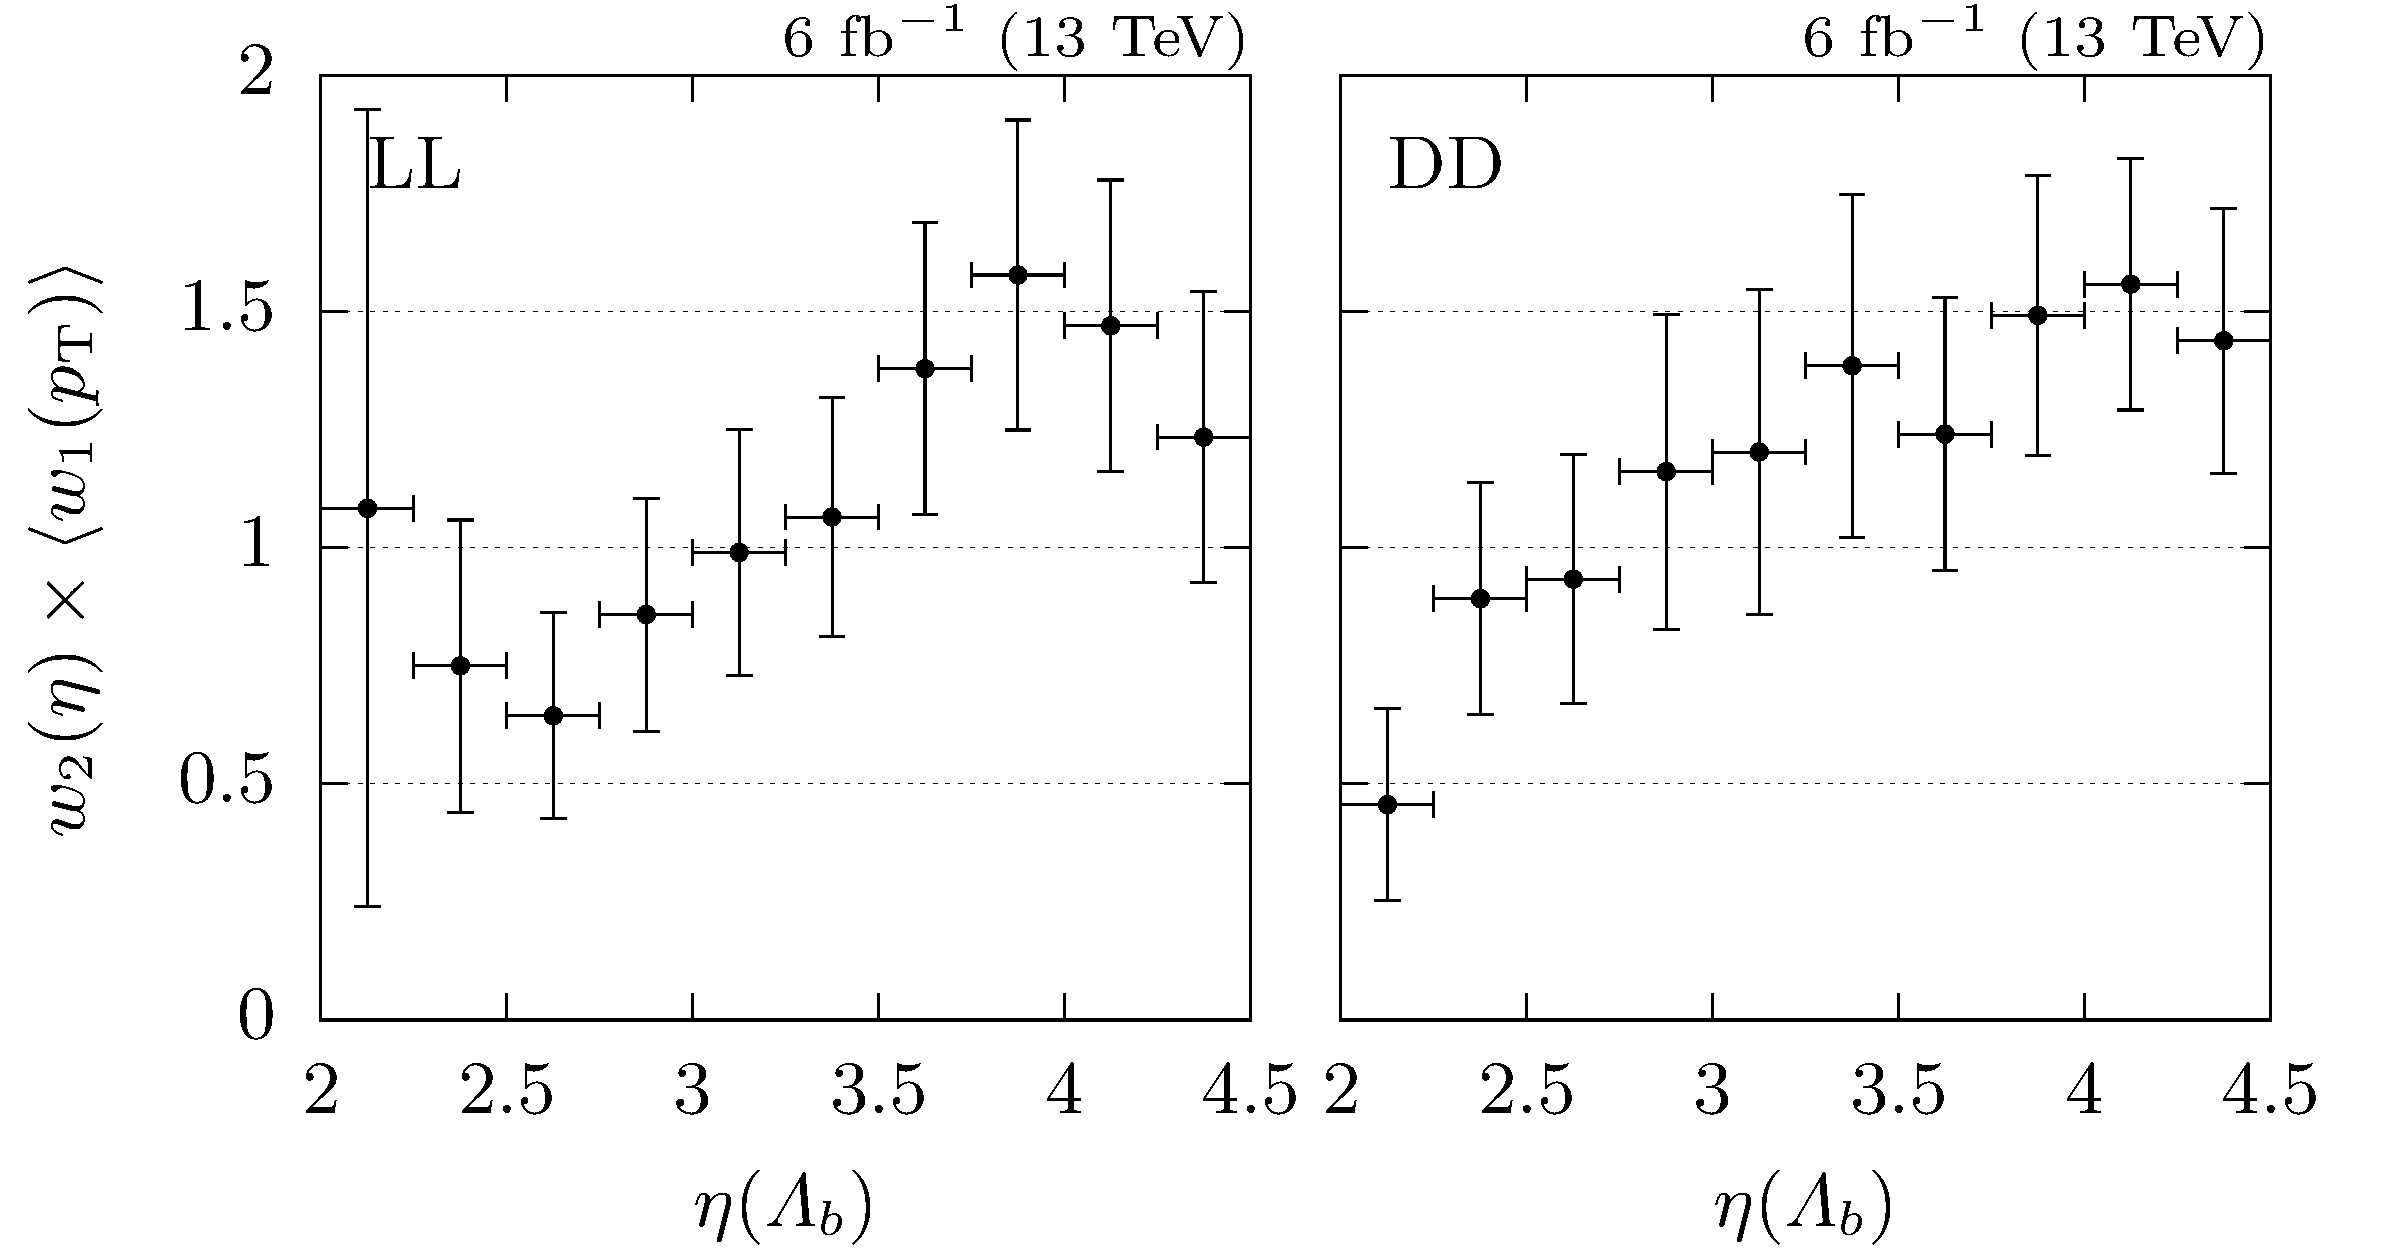
\includegraphics[scale=1.]{Lb2JpsiLz_weighting/avgw_prod_eta.png}
    \end{subfigure}
    \caption{Product of $w_1(\pt)$ and the mean of $w_2(\eta)$ (top) and vice versa (bottom) for \gls{LL} (left) and \gls{DD} (right) tracks.}
    \label{fig:LbToJpsiLz_avgw_prod}
\end{figure}

\begin{table}[htbp]
    \centering
    \caption{$p$-values w.r.t.\ the hypotheses $w_1(\pt)=1$ and $w_2(\eta)=1$ after six successive iterations, as well as the change of the $p$-value for $r(p)=1$, where $r(p)$ is the (binned) ratio of the three-momentum magnitude distribution of recorded data and simulated events, during the iterations.}
    \label{tab:LbToJpsiLz_pvalues}
    \begin{tabular}{ccc}
        \toprule
        & \gls{LL} & \gls{DD} \\
        \midrule
        $w_1(\pt)$ & $3\,\%$ & $0\,\%$ \\
        $w_2(\eta)$ & $71\,\%$ & $59\,\%$ \\
        \midrule
        $r(p)$ & $2\,\% \mapsto 53\,\%$ & $0\,\% \mapsto 24\,\%$ \\
        \bottomrule
    \end{tabular}
\end{table}

It is worthwhile to mention that the final weights do differ from the initial ratio of recorded and yet unweighted simulated events due to the correlation between \pt and $\eta$.
It is the product of $w_1(\pt)$ and $w_2(\eta)$ that will eventually reproduce the initially observed ratios, not the marginal distributions themself.
A visualization of this is given in the Fig.~\ref{fig:LbToJpsiLz_avgw_prod} that shows the product of $w_1(\pt)$ and the mean of $w_2(\eta)$ and vice versa for \gls{LL} and \gls{DD} tracks.

%\begin{figure}[htbp]
%    \centering
%    \begin{subfigure}{\textwidth}
%        \centering
%        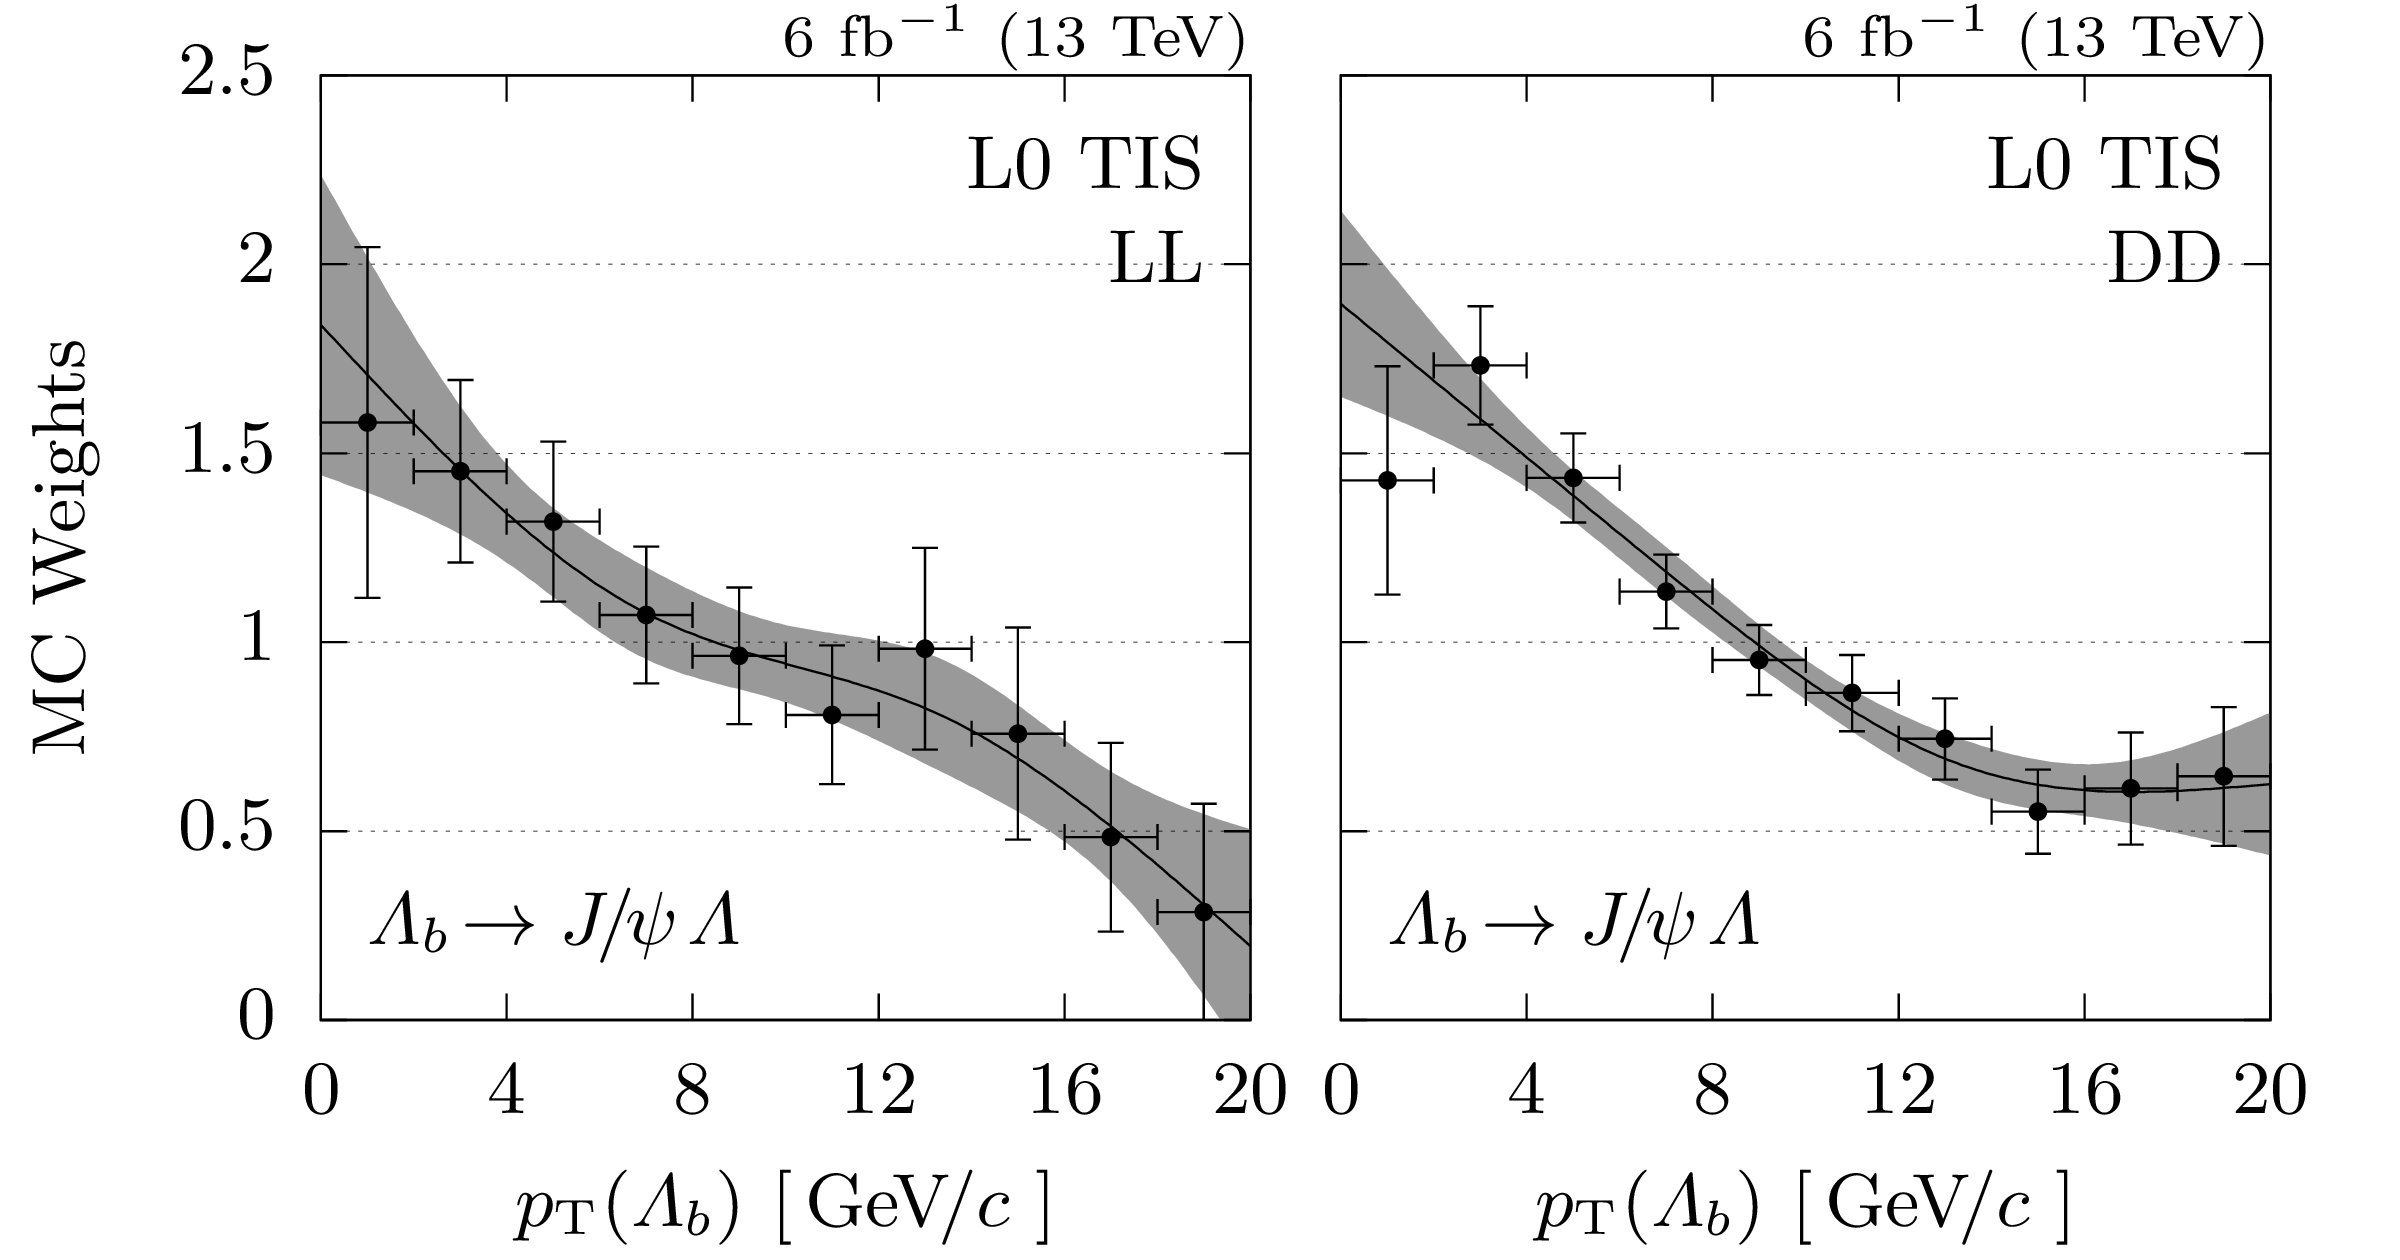
\includegraphics[scale=1.]{Lb2JpsiLz_weighting/weights_pT.png}
%    \end{subfigure}
%    \par\bigskip 
%    \begin{subfigure}{\textwidth}
%        \centering
%        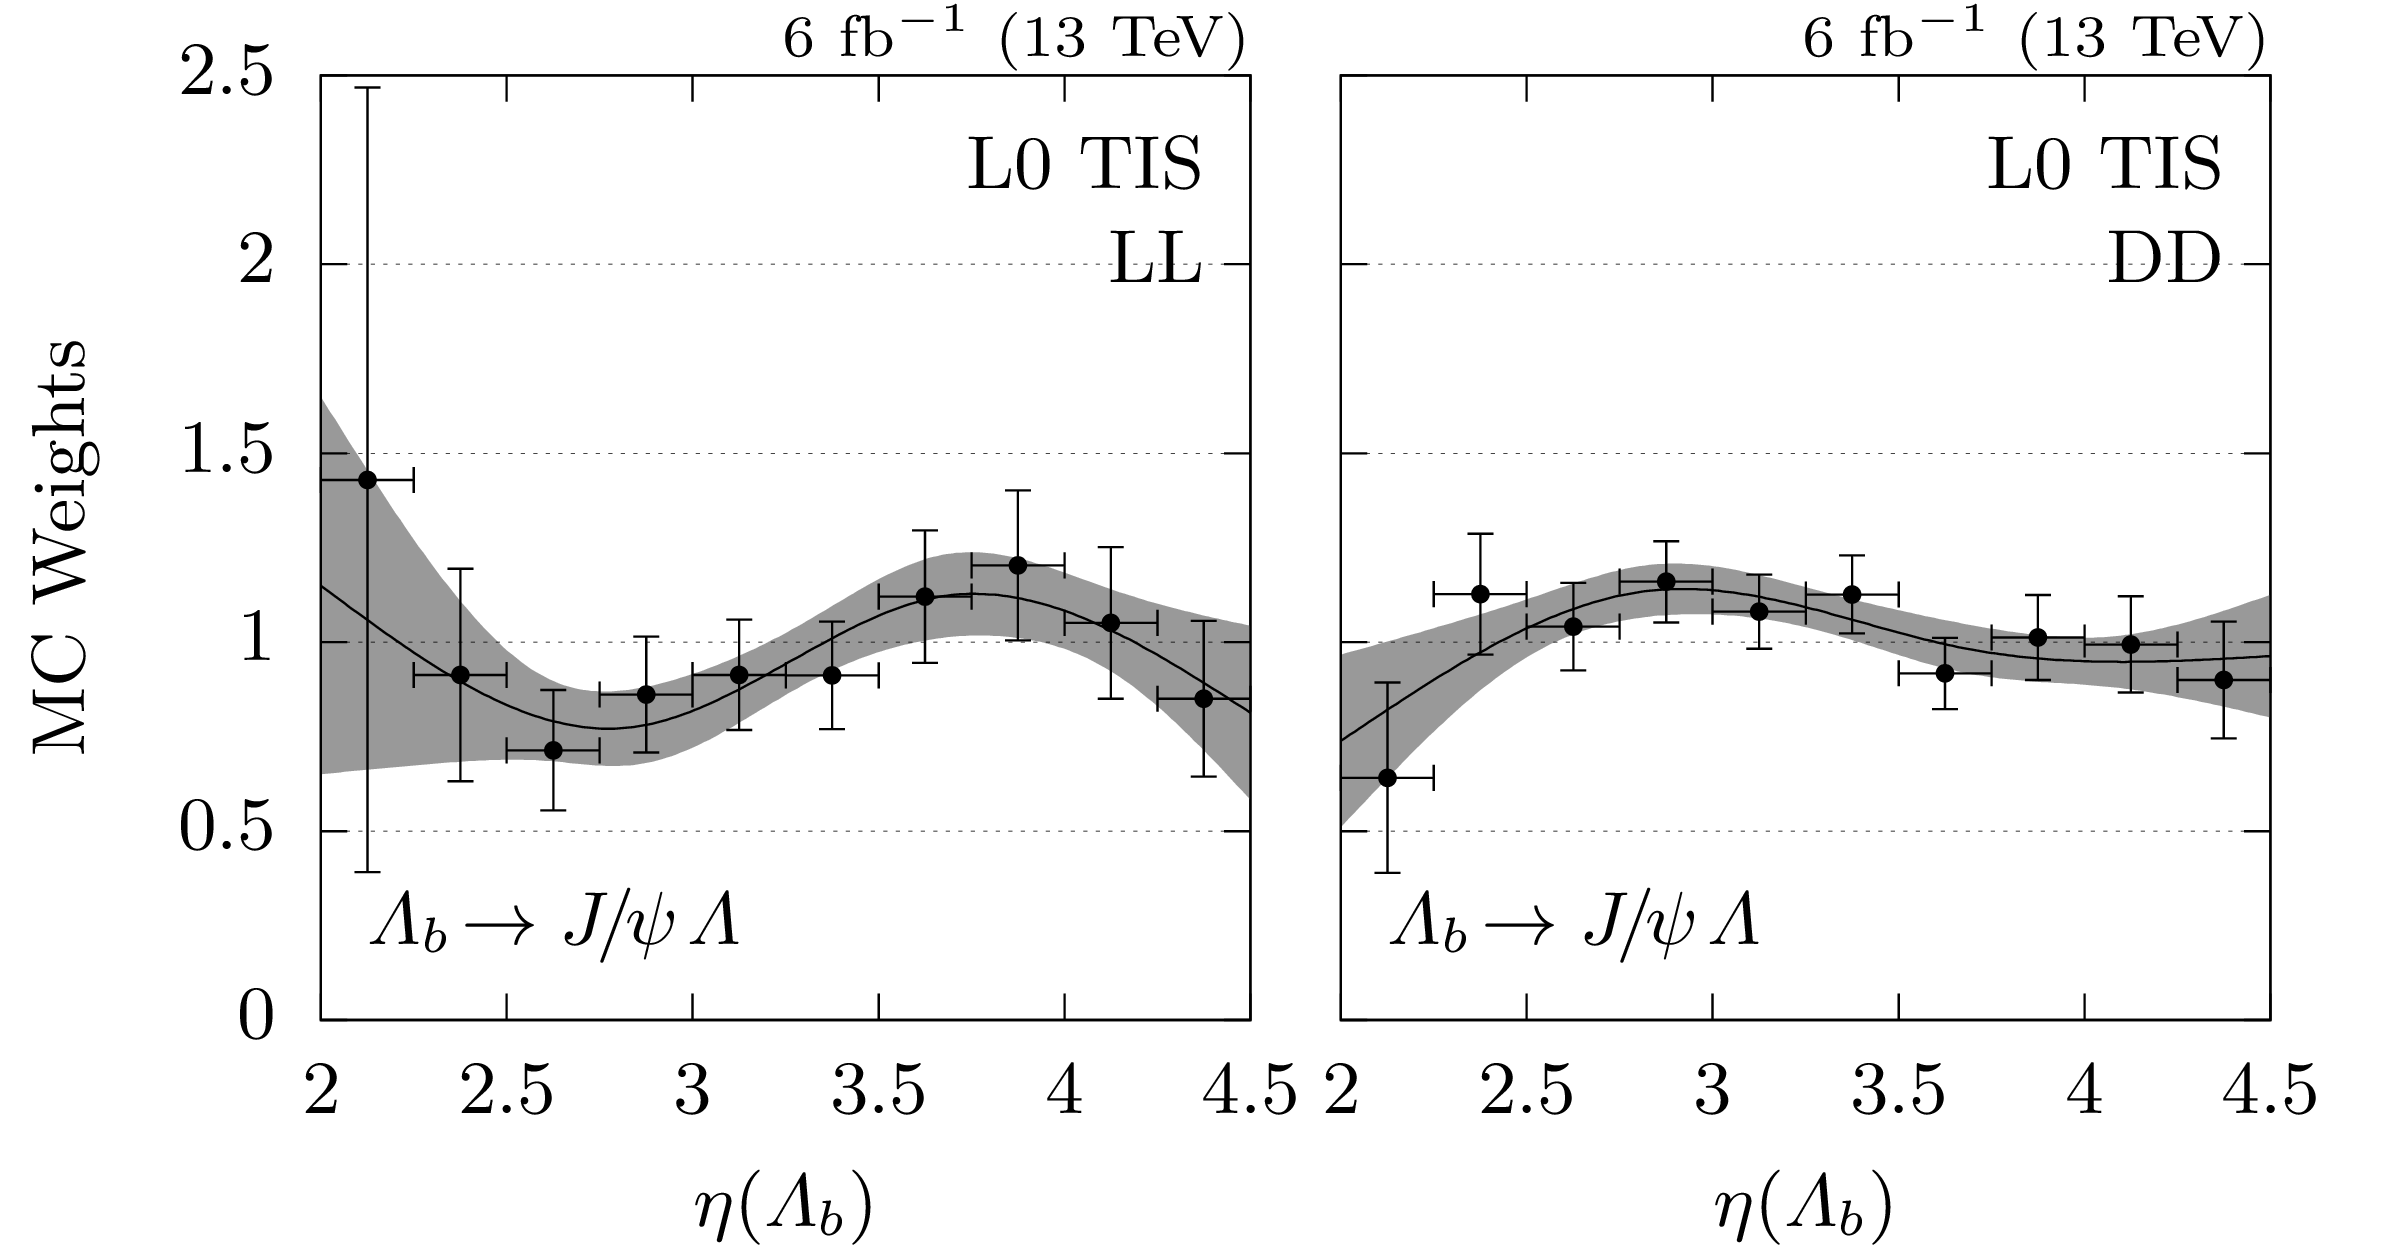
\includegraphics[scale=1.]{Lb2JpsiLz_weighting/weights_eta.png}
%    \end{subfigure}
%    \caption{Weights $w_1(\pt)$ (top) and $w_2(\eta)$ (bottom) for \gls{LL} (left) and \gls{DD} (right) tracks, as well as four independent equidistant (natural) cubic spline fits, each with four \gls{dof}.}
%    \label{fig:LbToJpsiLz_weights}
%\end{figure}

A priori, the distribution of weights cannot expected to be smooth, since each bin is corrected individually.
However, due to correlations, each \pt bin is linked to an entire set of $\eta$ bins and vice versa.
A correction of one bin will therefore also influence the weights of neighboring bins, hence a smoothing algorithm can be applied to reduce \gls{dof} and compensate uncertainties partially of each bin.

The separate weighting of \gls{LL} and \gls{DD} tracks was chosen, because doing so takes different selection criteria and heterogeneous sample sizes trivially into account.
However, separate weighting is not physically motivated, since the genuine \pt and $\eta$ distributions of $\Lb$ particles should be the same and independent of a specific decay mode or the track type of a \mbox{(grand-)daughter}.
In order to include this physical constraint back in, smoothing by fitting (natural) equidistant cubic splines with four \gls{dof} (\cf{}~Appx.~\ref{chap:csplines}) is performed separately for $w_1(\pt)$ and $w_2(\eta)$, but simultaneously for the different track types.
The resulting fits are shown in Fig.~\ref{fig:LbToJpsiLz_weights_simfit} together with the distributions of $w_1(\pt)$ and $w_2(\eta)$ and show an unphysical discrepancy between \gls{LL} and \gls{DD} tracks for $w_2(\eta)$.

%An equidistant (natural) cubic spline fit with four \gls{dof} is used to smooth $w_1(\pt)$ and $w_2(\eta)$ for both track types, separately.
%The result is shown in Fig.~\ref{fig:LbToJpsiLz_weights}.
%The discrepancy between \gls{LL} and \gls{DD} tracks for $w_2(\eta)$ is not physical since the true \pt and $\eta$ distributions of all $\Lb$ particles should be the same and independent of a specific decay mode or the track type of a (grand-)daughter.
%
\begin{figure}[htbp]
    \begin{subfigure}{\textwidth}
        \centering
        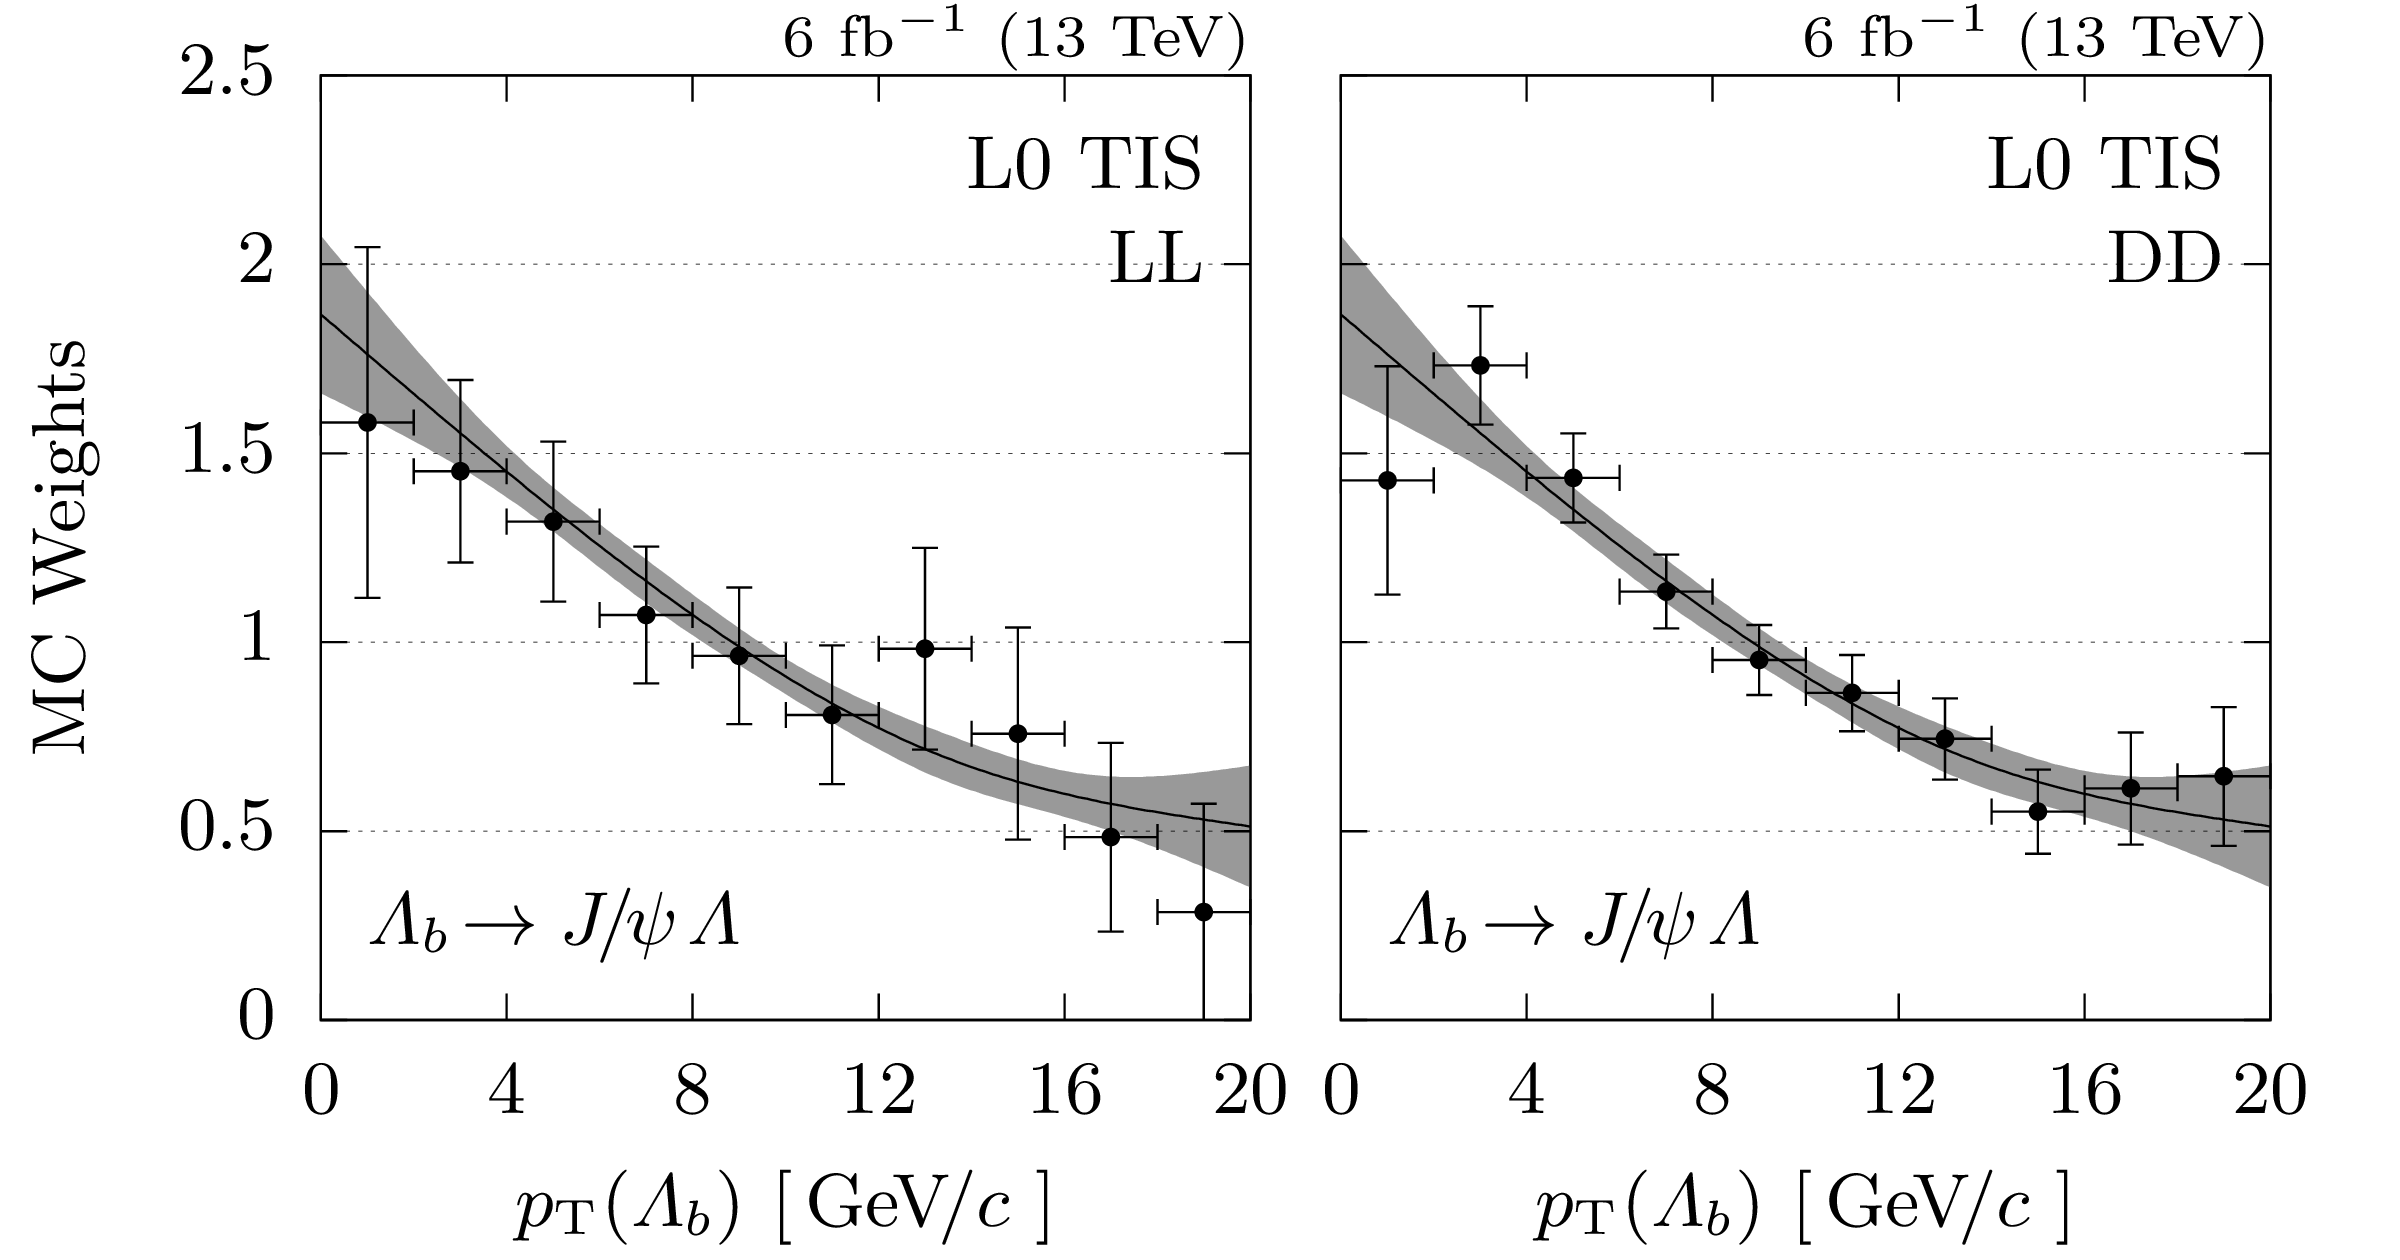
\includegraphics[scale=1.]{Lb2JpsiLz_weighting/weights_pT_simfit.png}
    \end{subfigure}
    \par\bigskip 
    \begin{subfigure}{\textwidth}
        \centering
        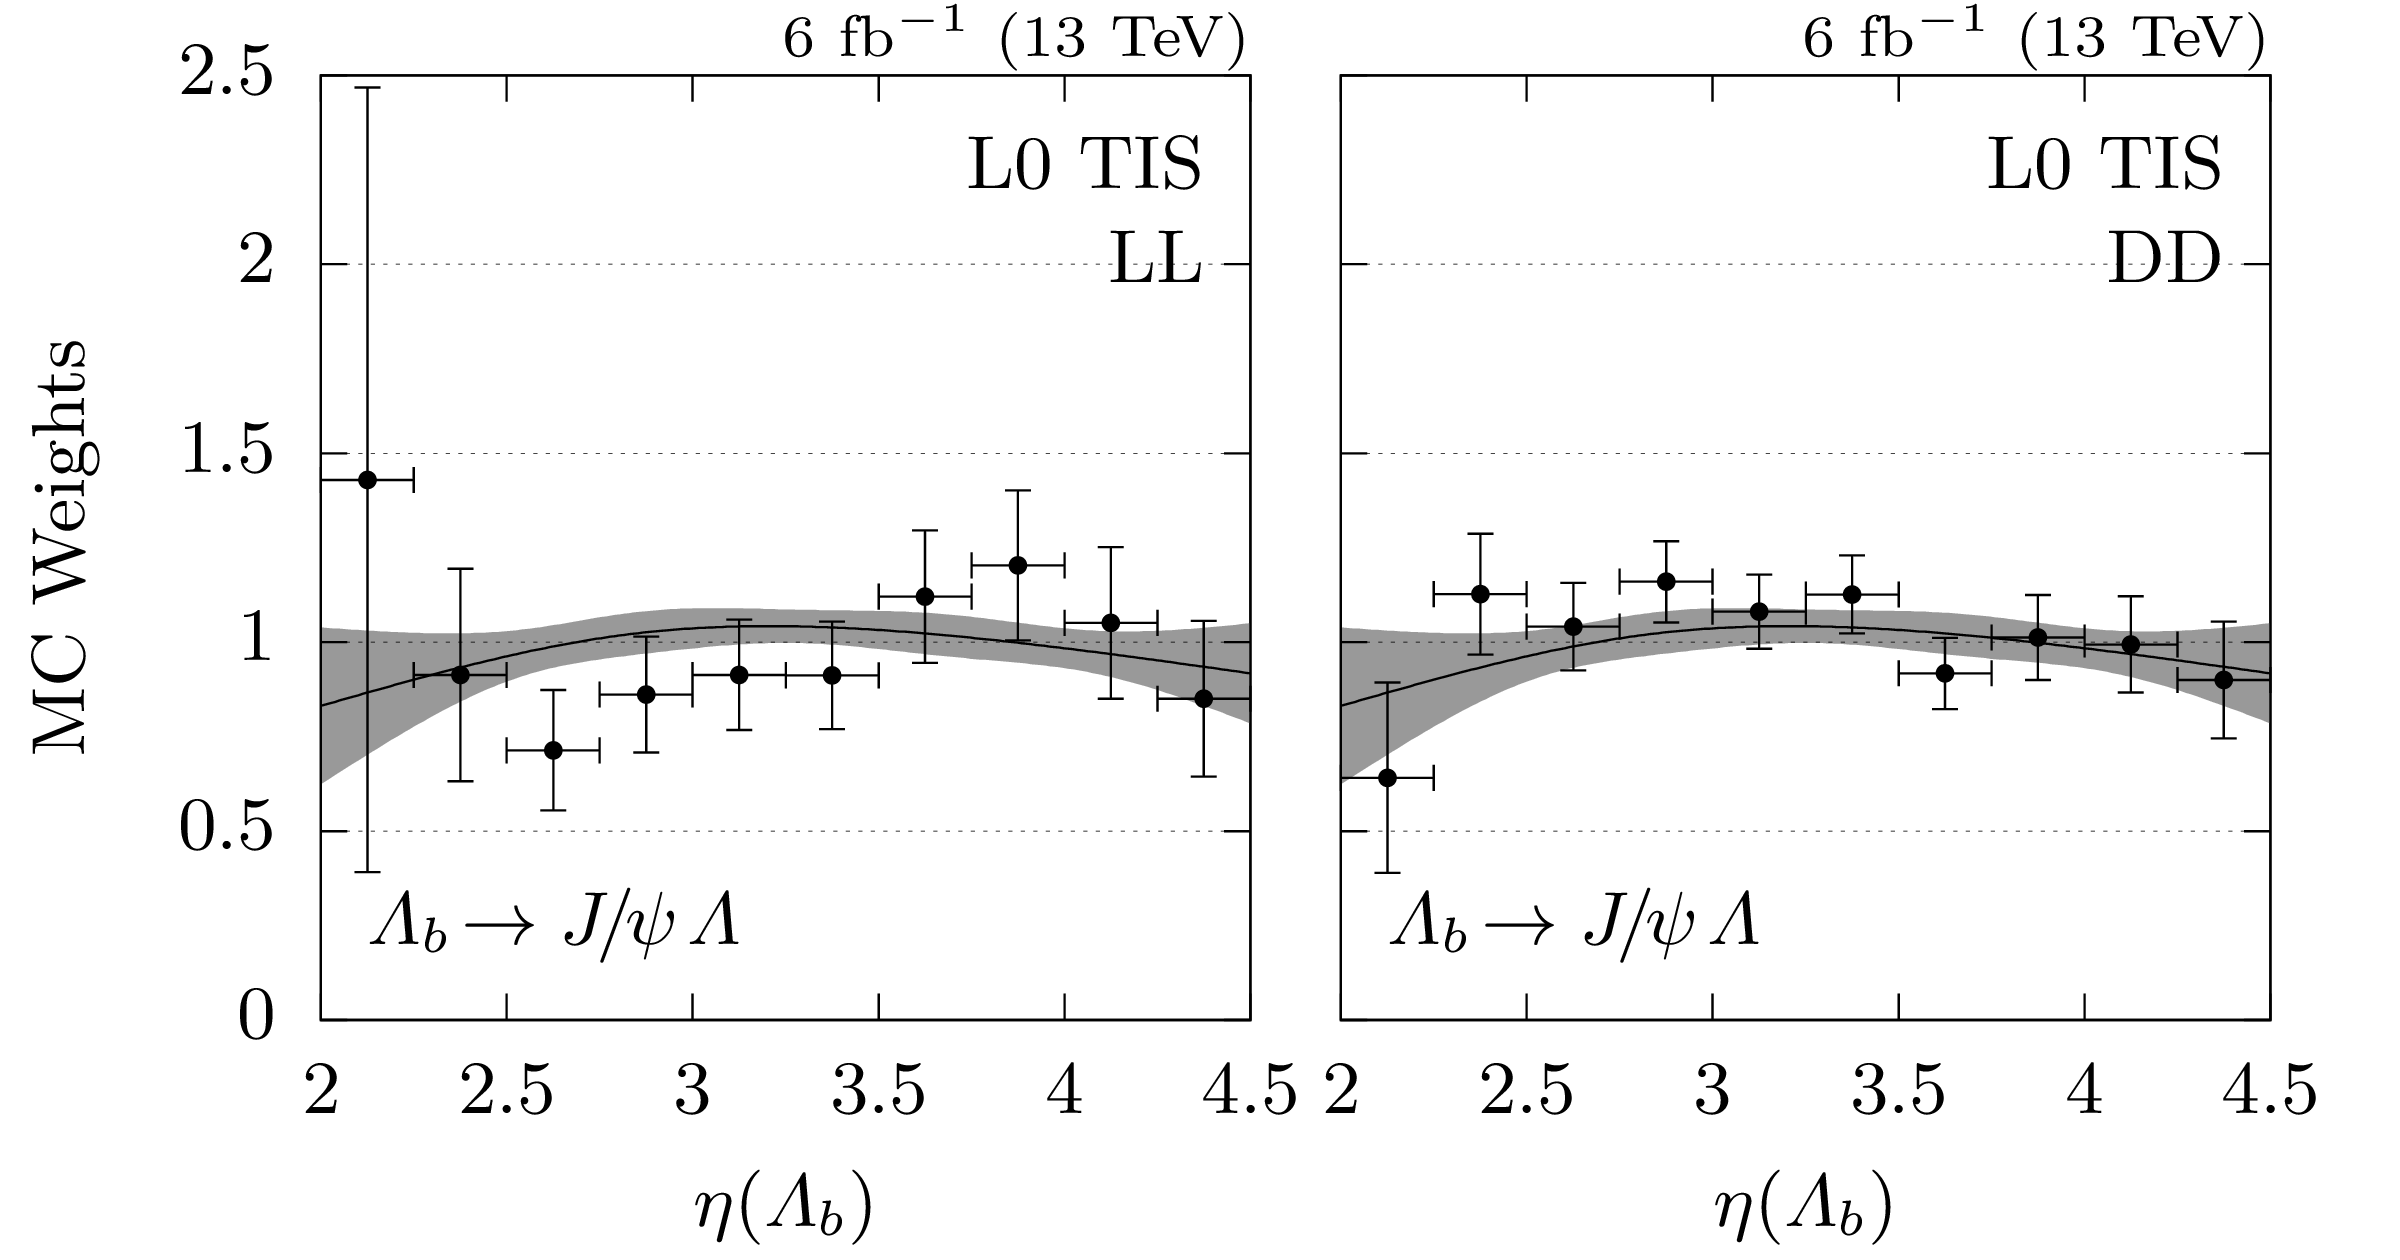
\includegraphics[scale=1.]{Lb2JpsiLz_weighting/weights_eta_simfit.png}
    \end{subfigure}
    \caption{Weights $w_1(\pt)$ (top) and $w_2(\eta)$ (bottom) for \gls{LL} (left) and \gls{DD} (right) tracks, as well as two equidistant (natural) cubic spline fits, each with four \gls{dof}. The distributions for \gls{LL} and \gls{DD} tracks are fitted simultaneously.}
    \label{fig:LbToJpsiLz_weights_simfit}
\end{figure}

\begin{figure}[htbp]
    \begin{subfigure}{\textwidth}
        \centering
        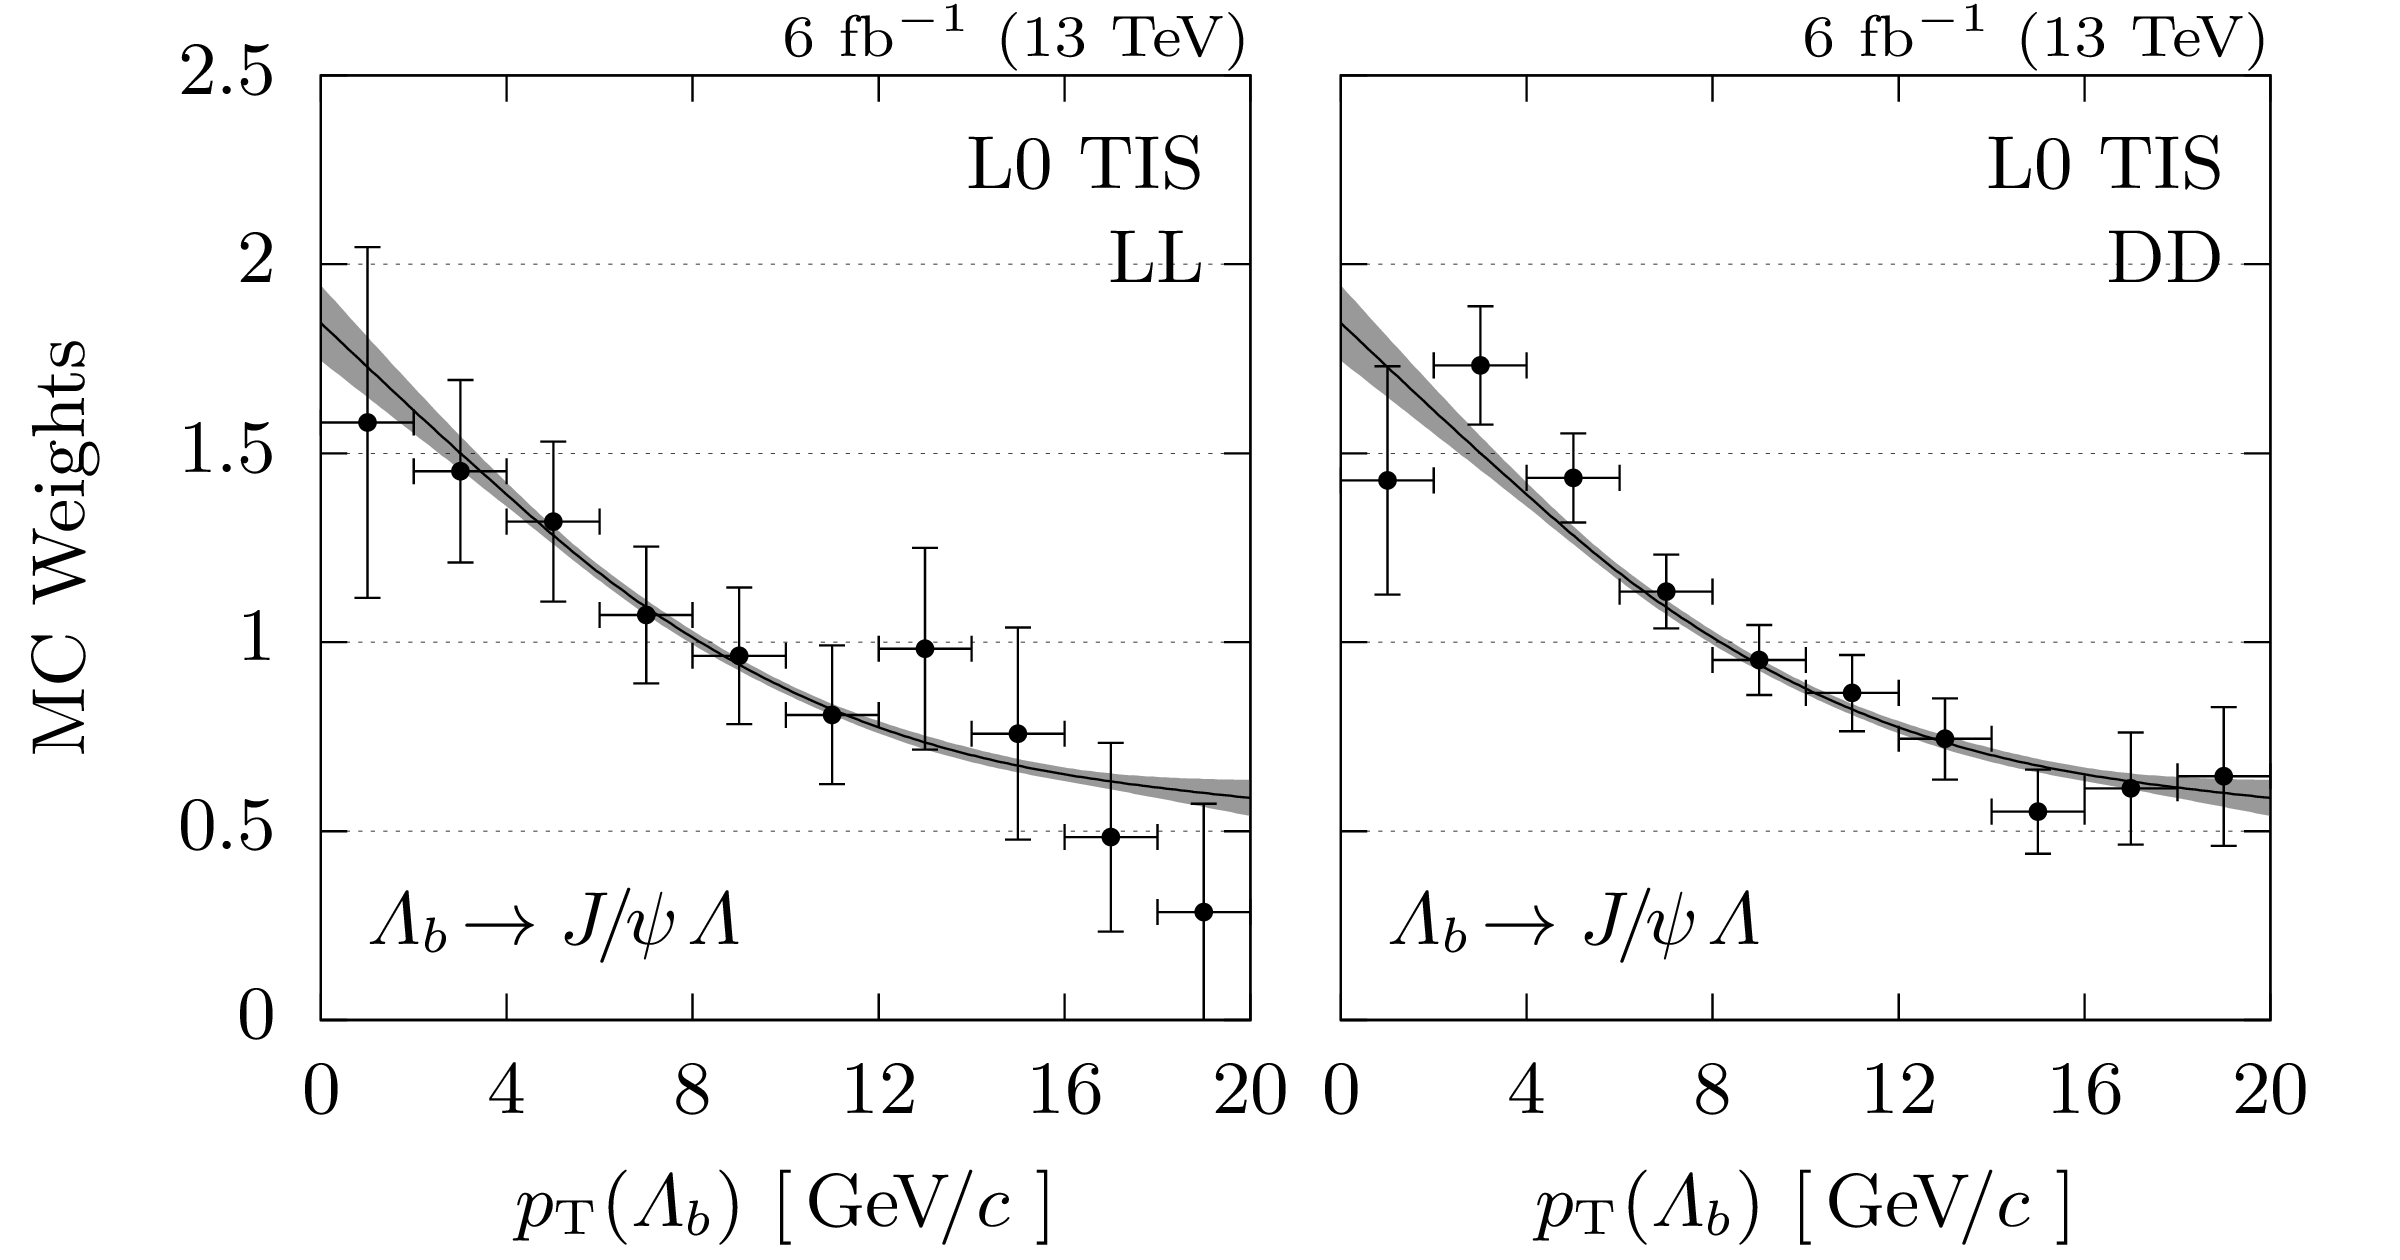
\includegraphics[scale=1.]{Lb2JpsiLz_weighting/weights_pT_avg.png}
    \end{subfigure}
    \par\bigskip 
    \begin{subfigure}{\textwidth}
        \centering
        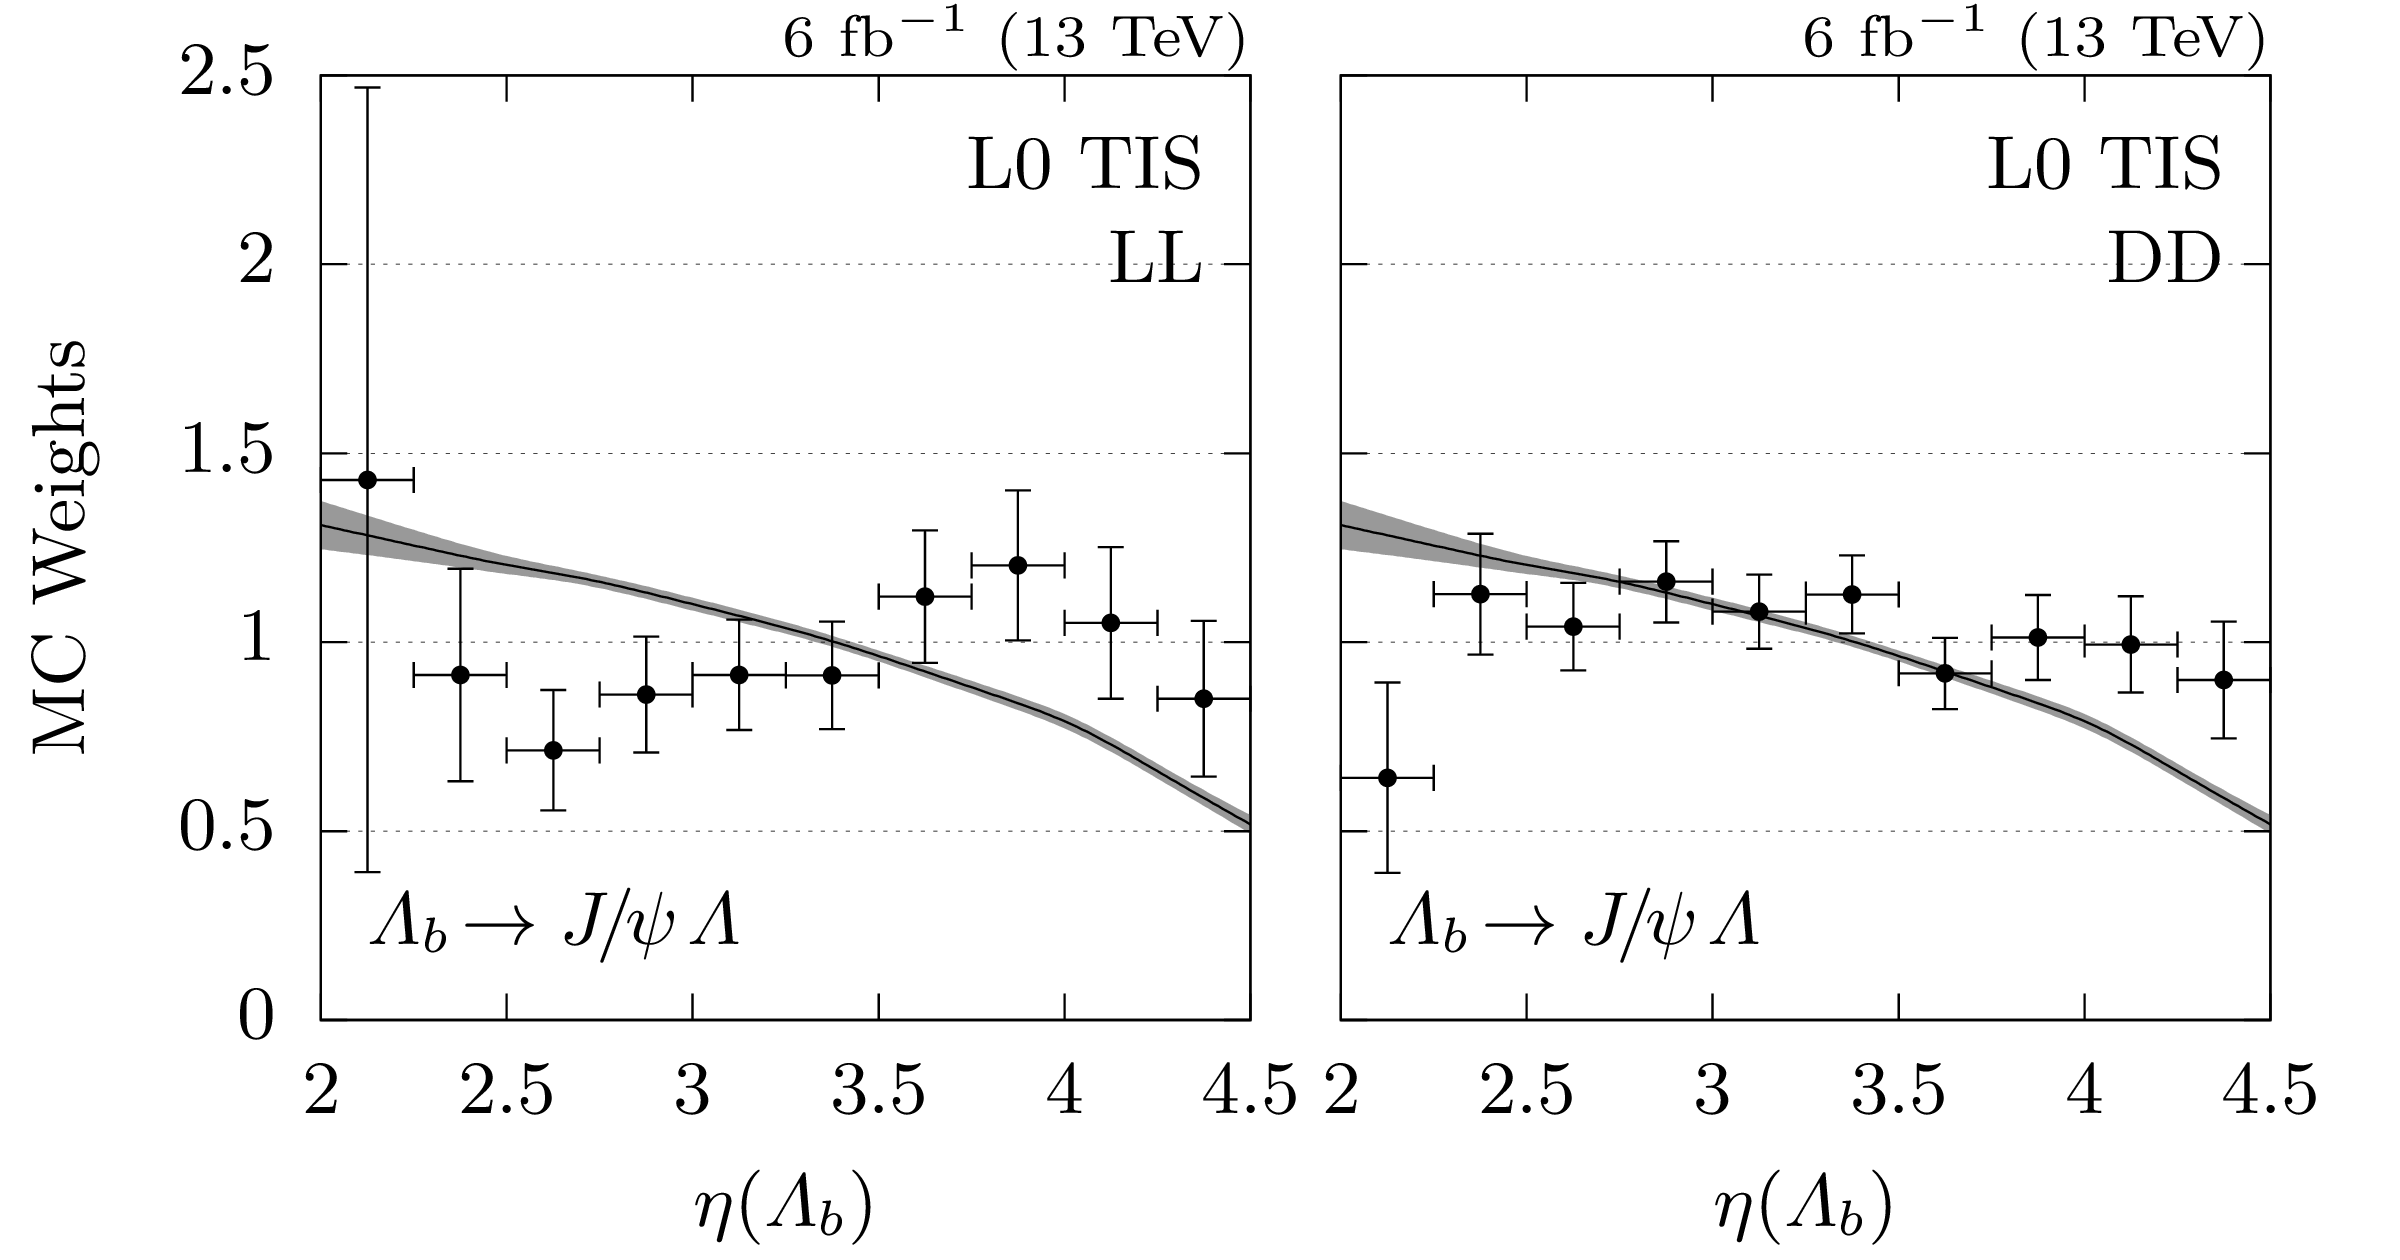
\includegraphics[scale=1.]{Lb2JpsiLz_weighting/weights_eta_avg.png}
    \end{subfigure}
    \caption{Averaged fit results of weights for \decay{\Lb}{\jpsi\Lz} (simultaneously for \gls{LL} and \gls{DD} tracks) and \decay{\Lb}{\Dz\proton\Km} events (taken from Ref.~\cite{hviemann}).}
    \label{fig:LbToJpsiLz_weights_avg}
\end{figure}

%The fit probability is approximately $99.7\,\%$ ($\chi^2 \approx 7$, \gls{dof}=$20$) and $83\,\%$ ($\chi^2 \approx 14$, \gls{dof}=$20$) for $w_1(\pt)$ and $w_2(\eta)$, respectively.

Since the weights $w_1(\pt)$ and $w_2(\eta)$ should neither depend on kinematic properties of \Lb daughters, nor on the decay channel itself, sensitivity is increased by combining our weights with weights extracted in a \decay{\Lb}{\Dz\proton\pim} analysis \cite{hviemann}.
(All final state particles are long tracks in this decay.)
We find a common set of weights by determining the weighted average of our simultaneously fitted $w(\pt, \eta)$ distribution and the corresponding one of the \decay{\Lb}{\Dz\proton\pim} analysis.
The fit results are shown in Fig.~\ref{fig:LbToJpsiLz_weights_avg} and exhibit a good agreement for $w_1(\pt)$, but large deviations for $w_2(\eta)$.
%(The latter predominantly arises from the larger statistics\footnote{The advantage of the higher statistics is compensated by the fact that the \decay{\Lb}{\jpsi\Lz} decay mode is much cleaner and easier to separate from background components.} of \decay{\Lb}{\Dz\proton\pim} at \lhcb.)
The combination reduces the statistical uncertainty and hints towards a difference between \gls{LL} and \gls{DD} that was already visible previously, but yet insignificant.
In comparison with the distributions of the non-normalized ratios of \gls{LL} and \gls{DD}, this difference is mostly promoted as an accumulation in the ratio of recorded and simulated data for \gls{LL} tracks and $\eta(\Lb) \gtrapprox 3.25$.

In Appx.~\ref{chap:apdx_weights} we summarize some investigations that exclude various possible explanations for the observed deviations in $w_2(\eta)$.
Eventually, the reason for this discrepancy stays unclear and motivates the second weighting scheme, outlined in the next section.

\subsection{Scheme 2}
\label{sec:LbToJpsiLz_w2}
In the considered sample of \decay{\Lb}{\jpsi\Lz} events, the weights $w_2(\eta)$ are compatible with one in good approximation, \cf{}~Tab.~\ref{tab:LbToJpsiLz_pvalues}.
Hence, a conservative approximation is to use $w(p_T, \eta) = 1 \times w'_2(p_T)$.
Since $p_T(\Lb)$ and $\eta(\Lb)$ are correlated, it is not sufficient to simply set $w_2(p_T) \equiv w_2'(p_T)$ in $w(p_T, \eta) = w_1(p_T) \times w_2(\eta)$.
Instead the ratio of recorded data and unweighted simulated events is taken as weights.
(Since there is only one variable, there is no need to perform this in an iterative approach.)

\begin{figure}[htbp]
    \centering
    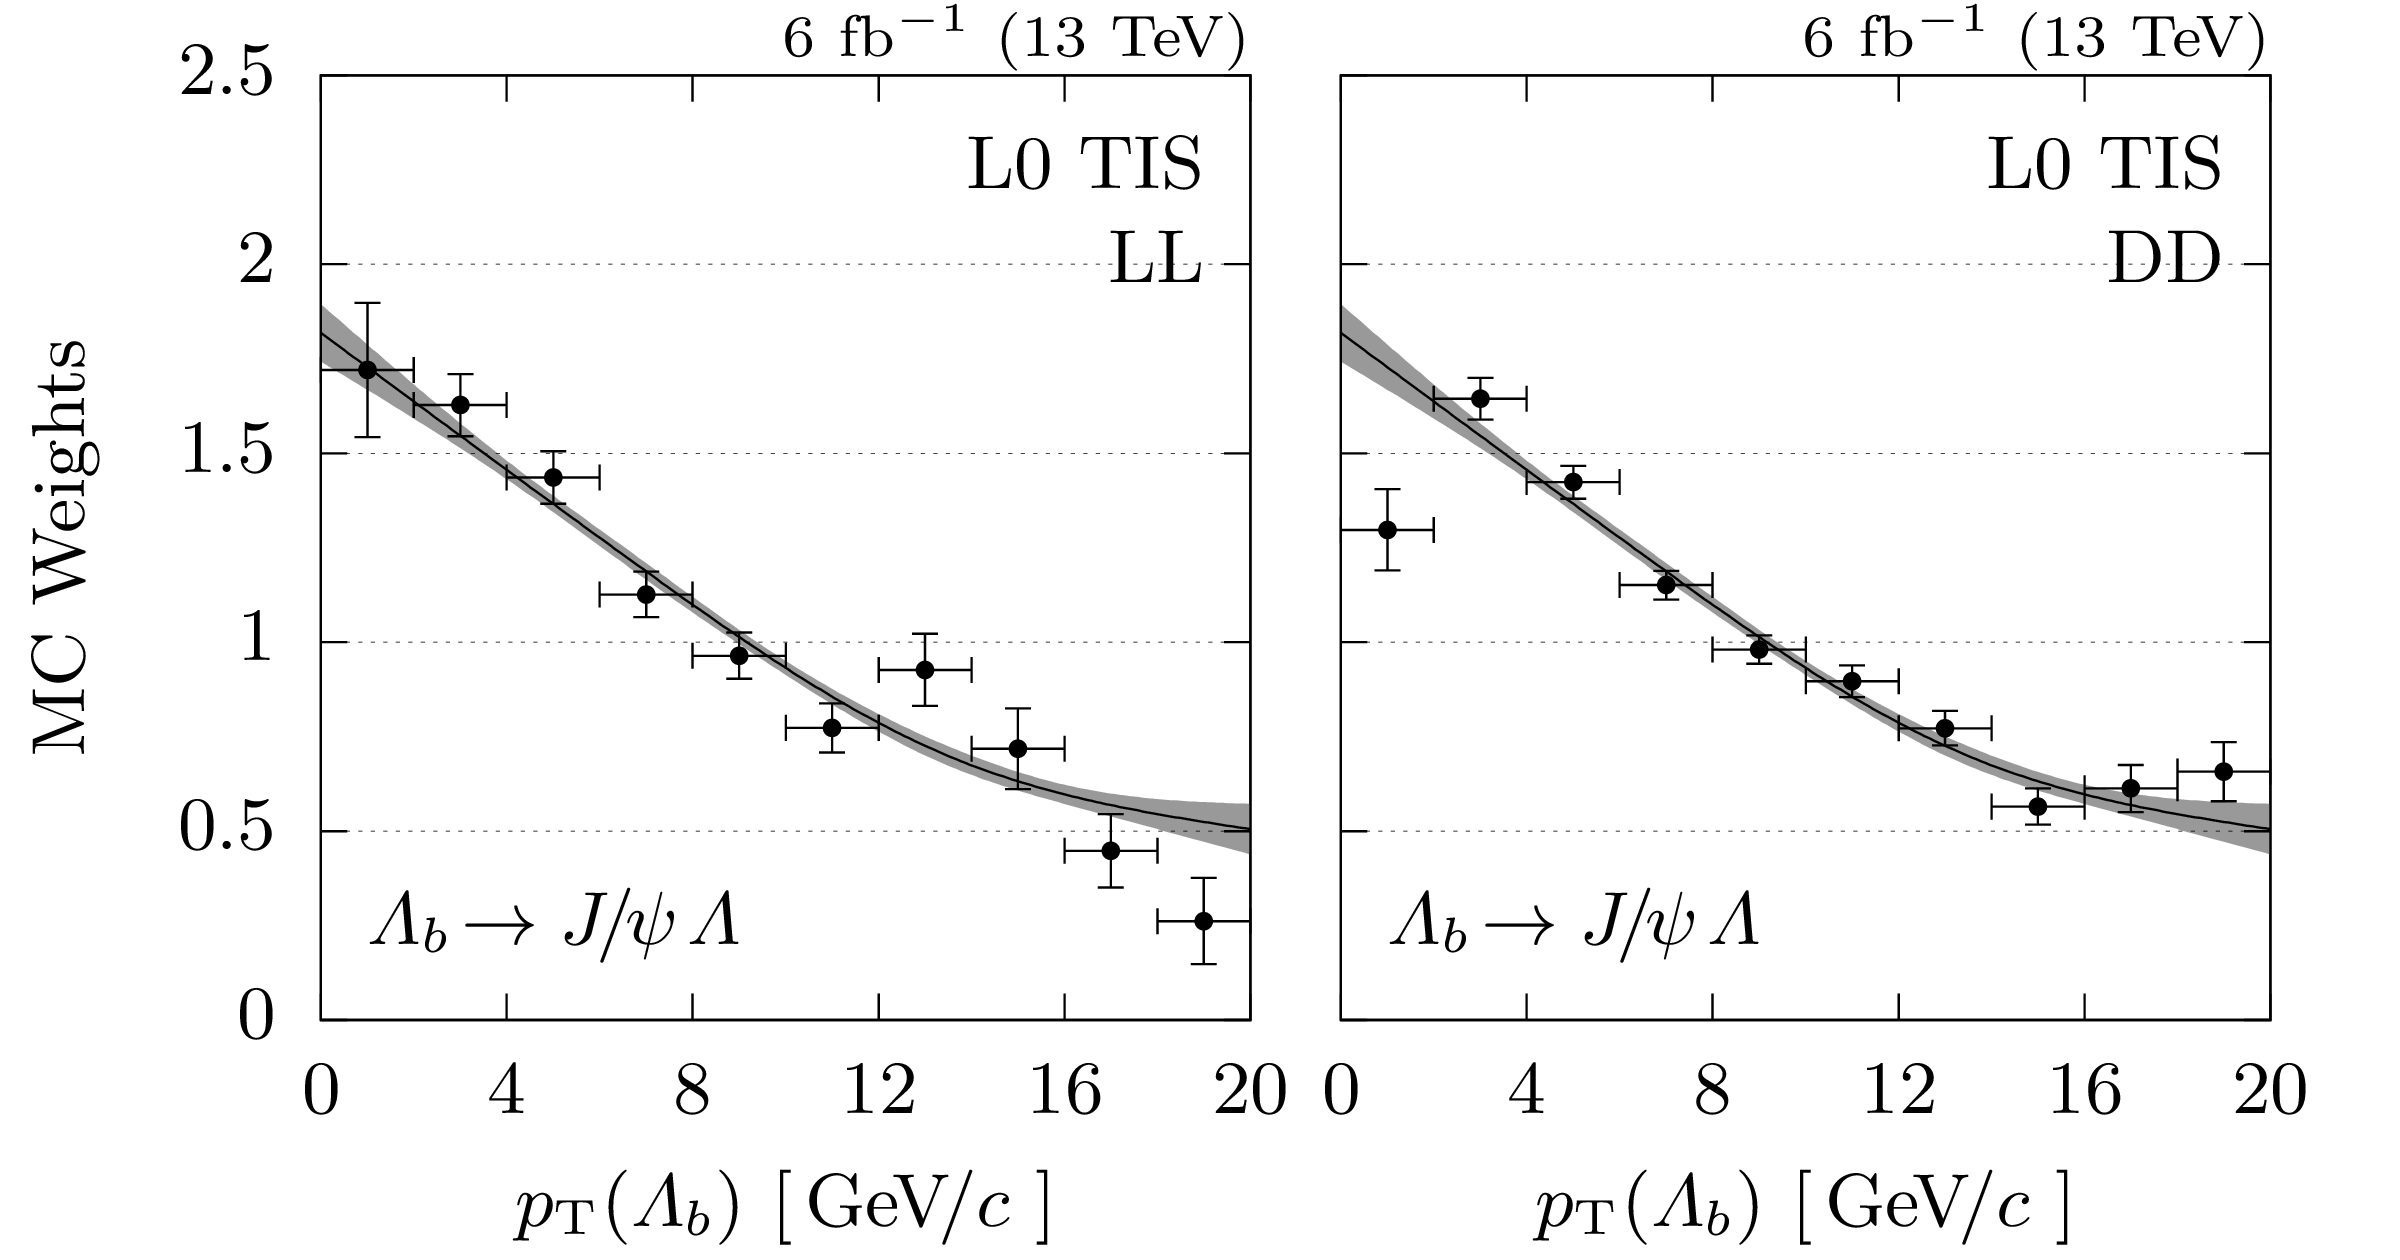
\includegraphics[scale=1.]{Lb2JpsiLz_weighting/weights_altfit.png}
    \caption{$\pt$-dependent weights obtained by weighting scheme 2, as well as spline fit, evaluated simultaneously for \gls{LL} and \gls{DD} tracks.}
    \label{fig:LbToJpsiLz_weights_altfit}
\end{figure}

The ratios are smoothed using a (natural) cubic spline with four \gls{dof} (\cf{}~Appx.~\ref{chap:csplines}).
Again, the spline is fitted simultaneously to \gls{LL} and \gls{DD} tracks.
Subsequently, the smoothed weights are used to weight the \gls{mc} simulated events.
The resulting distributions, as well as the corresponding spline fits for $\pt(\Lb)$ and both track types are shown in Fig.~\ref{fig:LbToJpsiLz_weights_altfit}.

In Fig.~\ref{fig:LbToJpsiLz_hratio_altfinal} we show the ratio of recorded data and weighted \gls{mc} simulated events for $\pt(\Lb)$ and $p(\Lb)$.
The combined $p$-values for both track types w.r.t.\ the hypothesis of a common underlying distribution for recorded and simulated events are approximately $8\,\%$ ($\chi^2 \approx 30$) and $0.1\,\%$ ($\chi^2 \approx 45$) for the $p(\Lb)$ and $\pt(\Lb)$ distributions, respectively.
These values do not include uncertainties of the spline fit and thus reflect only the $p$-value for a specific choice of weighting function.

\begin{figure}[htbp]
    \centering
    \begin{subfigure}{\textwidth}
        \centering
        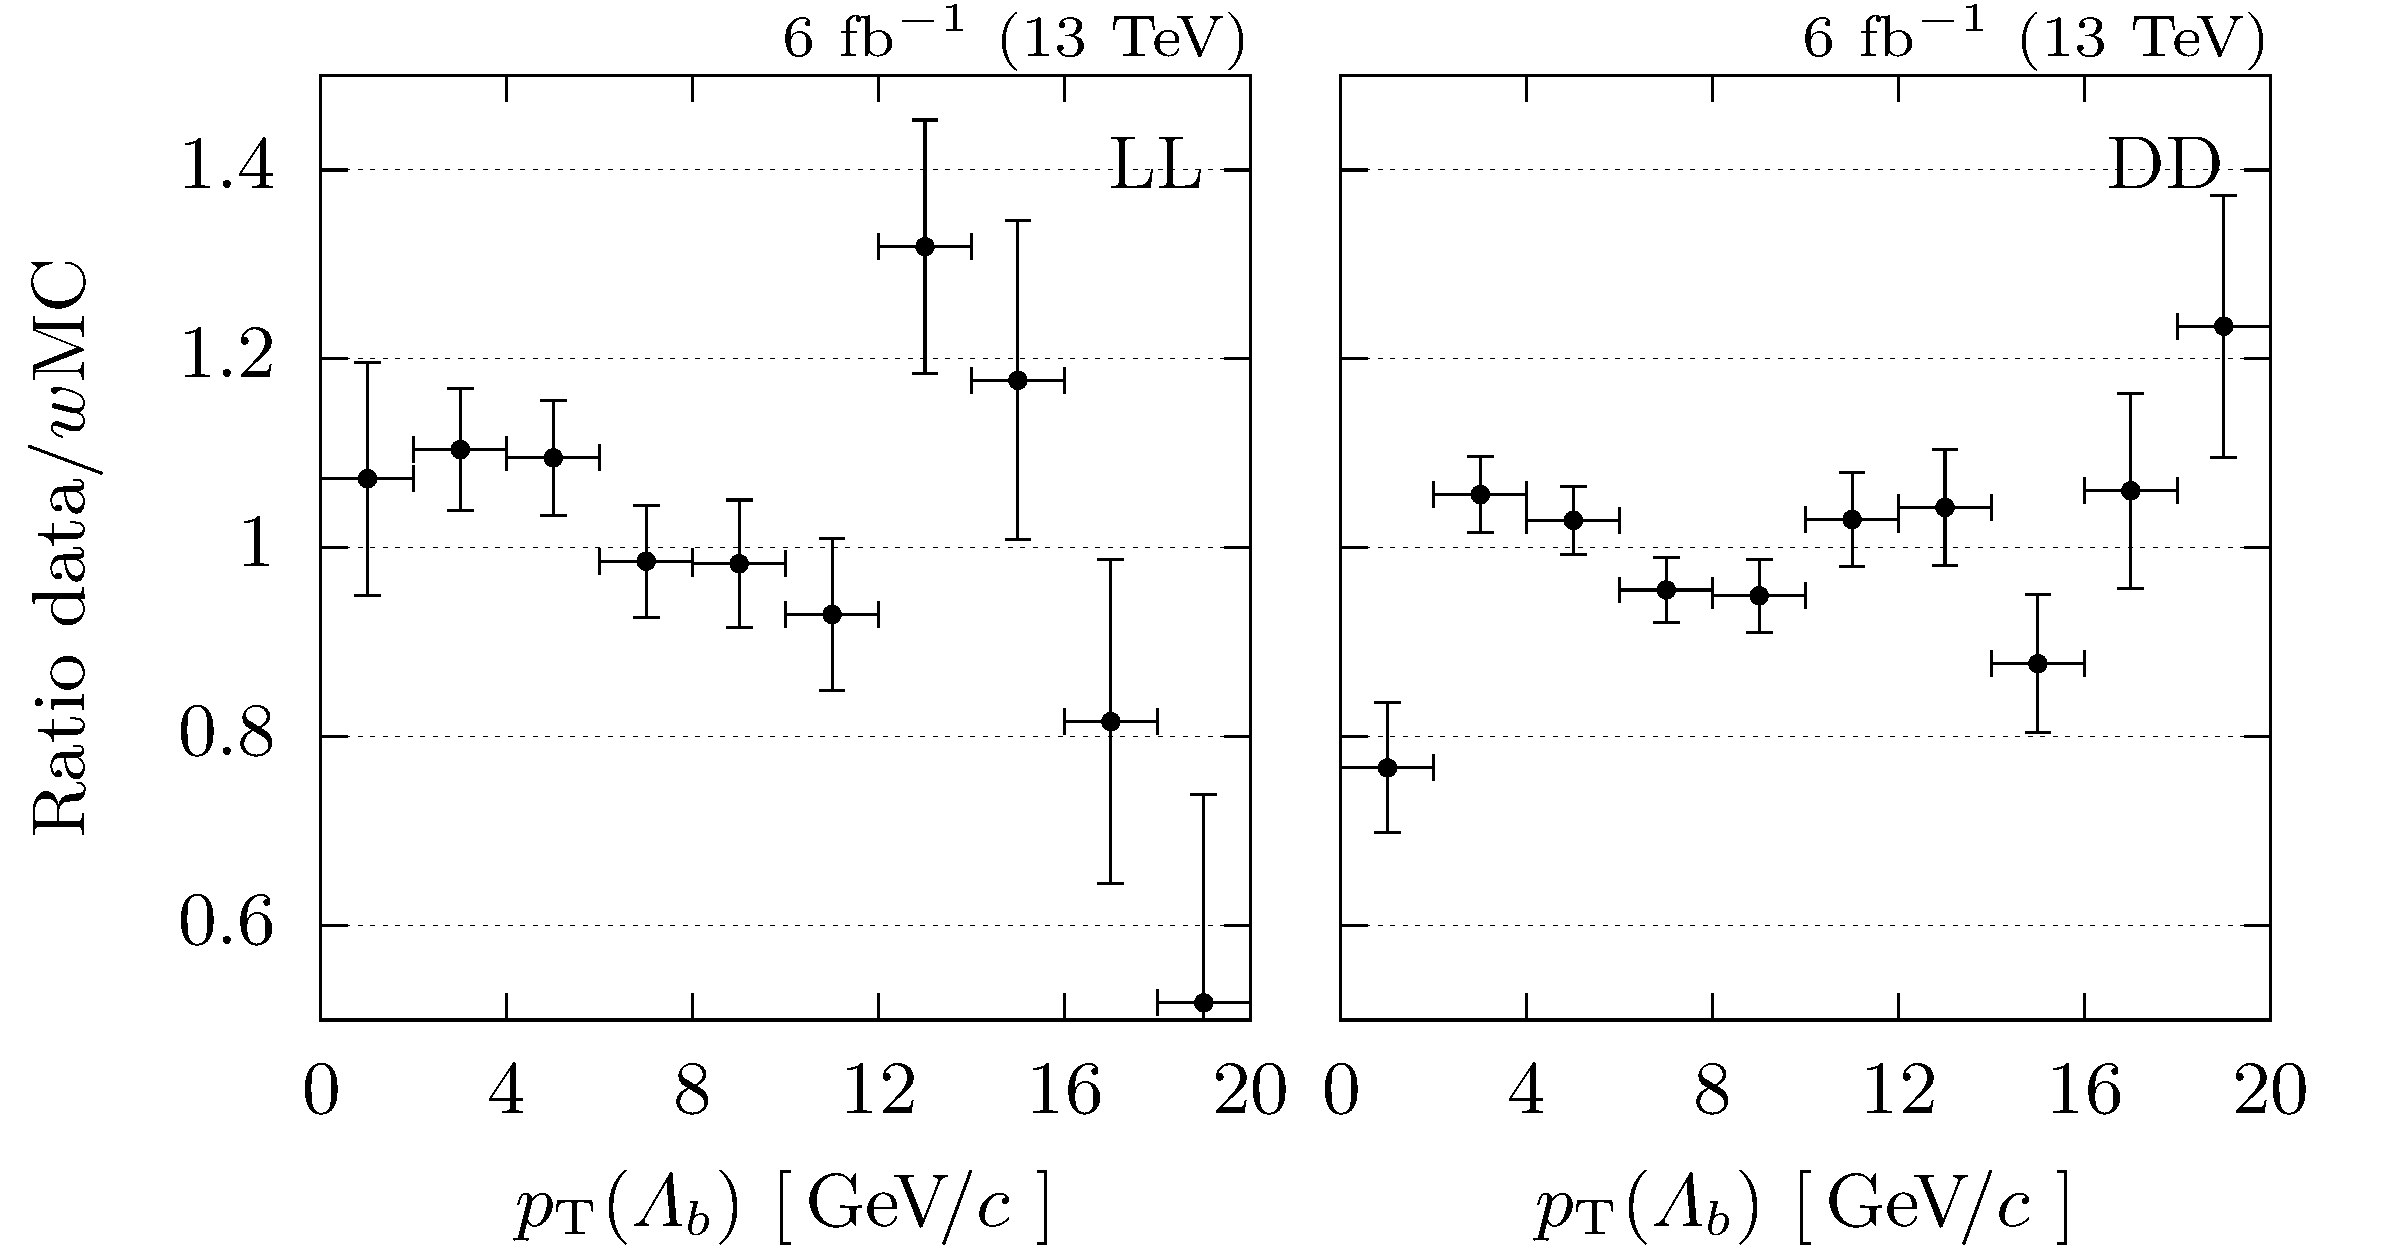
\includegraphics[scale=1.]{Lb2JpsiLz_weighting/hratio_pT_altfinal.png}
    \end{subfigure}
    \par\bigskip 
    \begin{subfigure}{\textwidth}
        \centering
        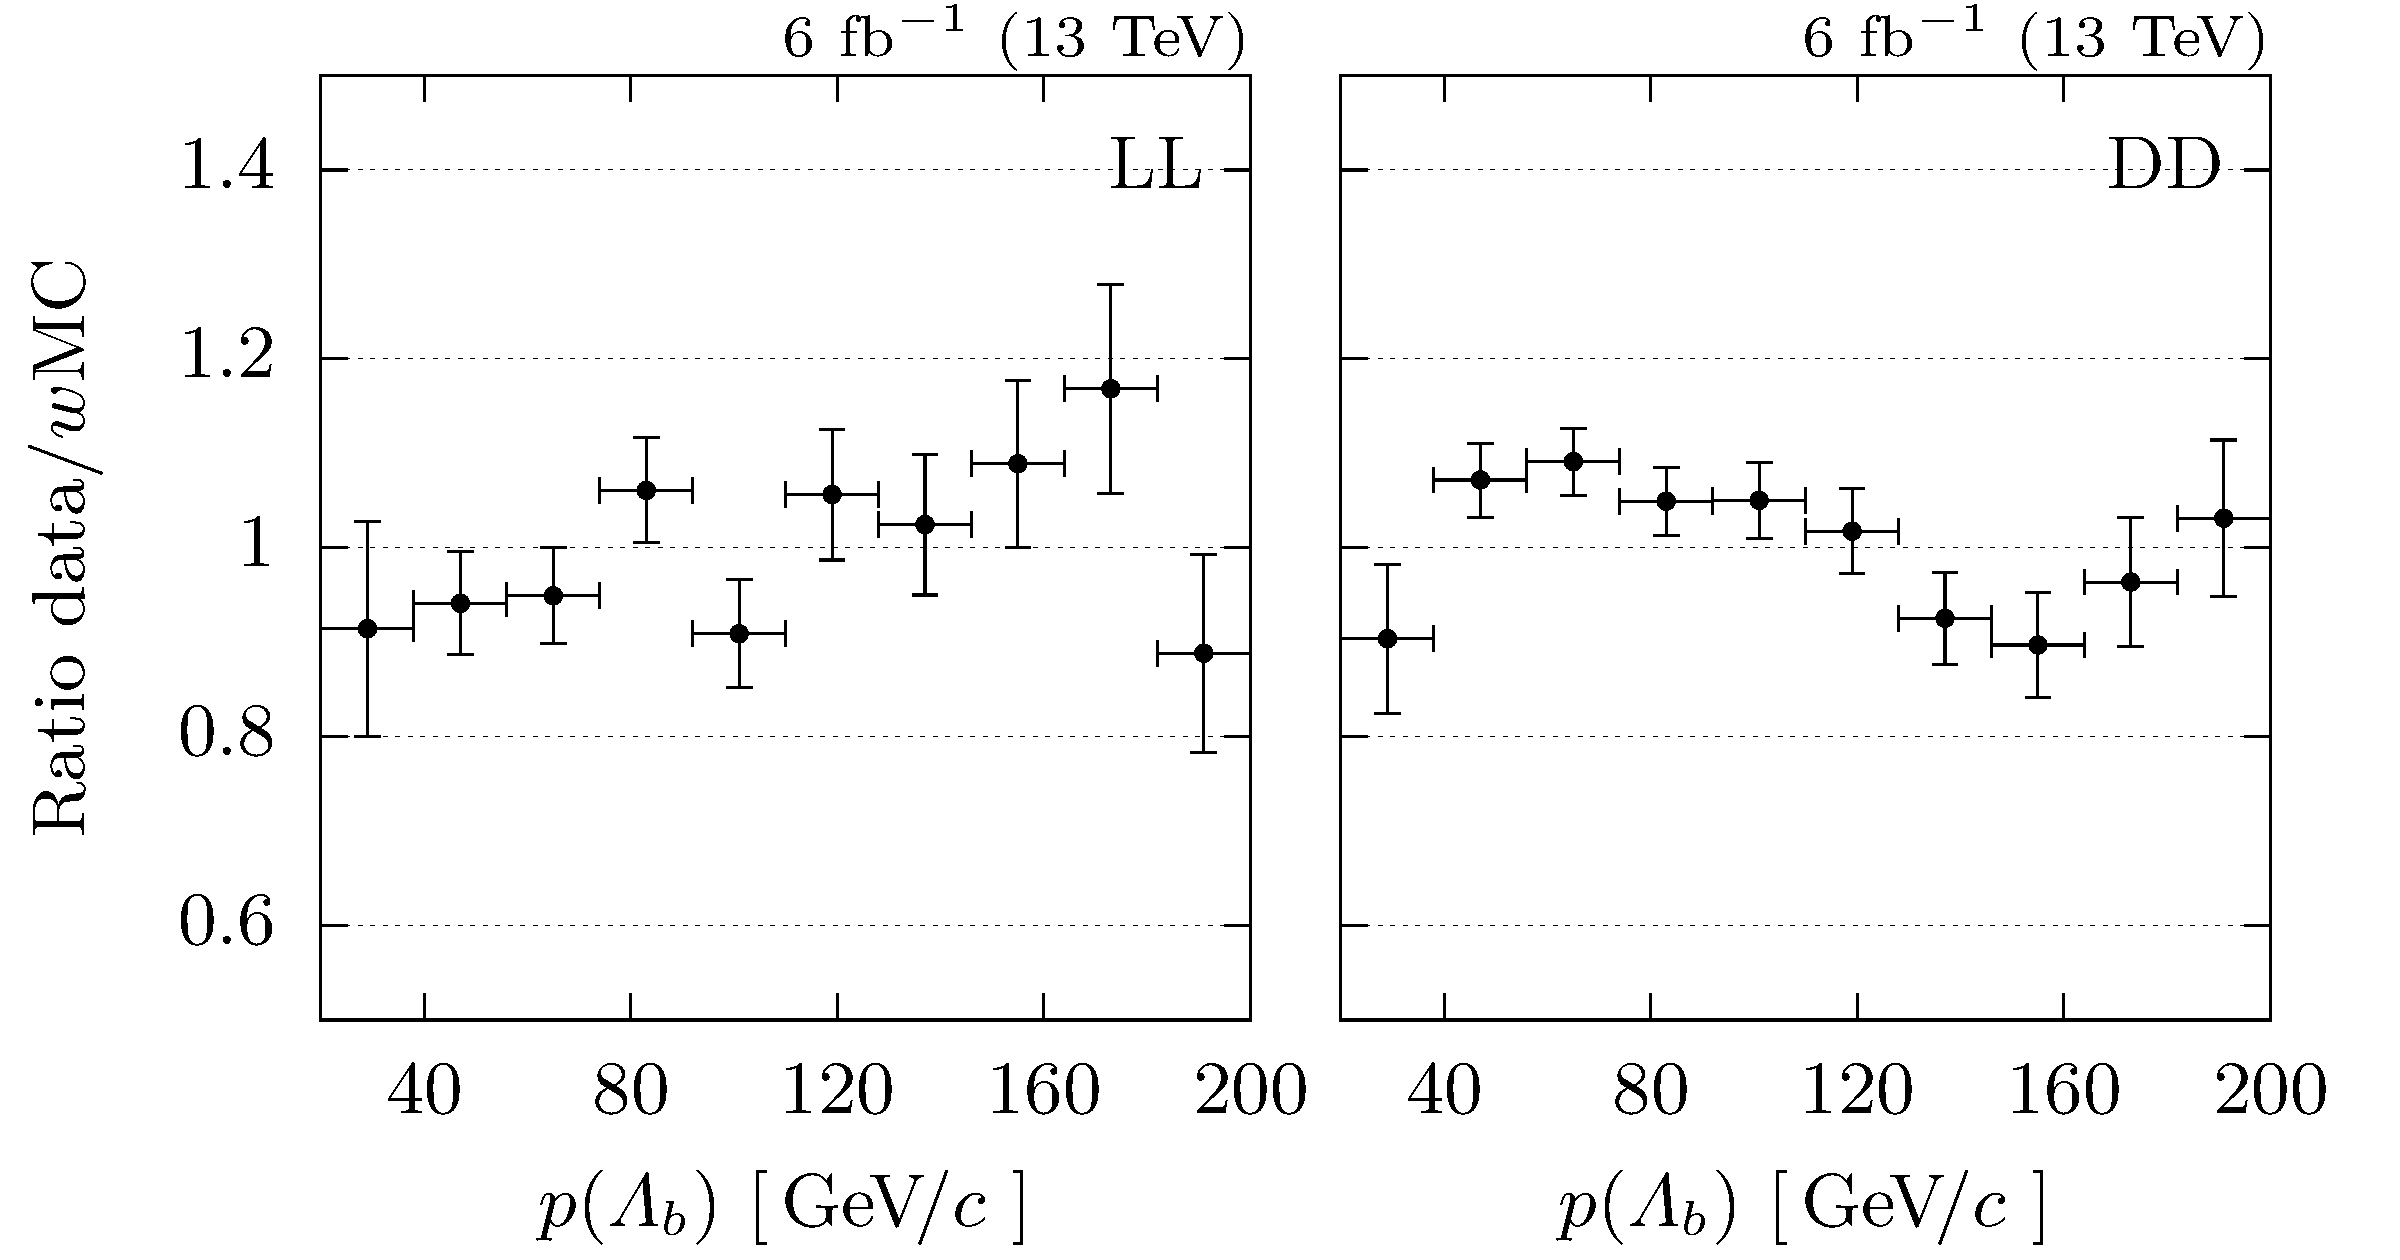
\includegraphics[scale=1.]{Lb2JpsiLz_weighting/hratio_p_altfinal.png}
    \end{subfigure}
    \caption{Ratio of recorded data and weighted \gls{mc} simulated events according to weighting scheme 2 for the transverse momentum of the \Lb baryon $\pt(\Lb)$ (top) and its three-momentum magnitude $p(\Lb)$ (bottom).}
    \label{fig:LbToJpsiLz_hratio_altfinal}
\end{figure}
